%  LaTeX support: latex@mdpi.com
%  In case you need support, please attach all files that are necessary for compiling as well as the log file, and specify the details of your LaTeX setup (which operating system and LaTeX version / tools you are using).

% You need to save the "mdpi.cls" and "mdpi.bst" files into the same folder as this template file.

%=================================================================
\documentclass[electronics,article,accept,moreauthors,pdftex,10pt,a4paper]{mdpi}
\synctex=1
\usepackage{fixme}
\usepackage{caption}
\usepackage{subcaption}
\usepackage{listings}             % Include the listings-package
\usepackage{placeins}
\usepackage{xcolor}
\usepackage{caption}
\usepackage{textcomp}  % To get the correct quotes in lstlistings (')
\usepackage{appendix}
\usepackage{soul}



\newcommand\floor[1]{\left\lfloor#1\right\rfloor}
\newcommand\ceil[1]{\left\lceil#1\right\rceil}

\newcommand{\todot}[1]{%
  \textbf{\textcolor{red}{TO DO: #1}}
}

%--------------------
% Class Options:
%--------------------
% journal
%----------
% Choose between the following MDPI journals:
% actuators, admsci, aerospace, agriculture, agronomy, algorithms, animals, antibiotics, antibodies, antioxidants, applsci, arts, atmosphere, atoms, axioms, batteries, behavsci, beverages, bioengineering, biology, biomedicines, biomimetics, biomolecules, biosensors, brainsci, buildings, carbon, cancers, catalysts, cells, challenges, chemosensors, children, chromatography, climate, coatings, computation, computers, condensedmatter, cosmetics, cryptography, crystals, data, dentistry, designs, diagnostics, diseases, diversity, econometrics, economies, education, electronics, energies, entropy, environments, epigenomes, fermentation, fibers, fishes, fluids, foods, forests, futureinternet, galaxies, games, gels, genealogy, genes, geosciences, geriatrics, healthcare, horticulturae, humanities, hydrology, informatics, information, infrastructures, inorganics, insects, instruments, ijerph, ijfs, ijms, ijgi, inventions, jcdd, jcm, jdb, jfb, jfmk, jimaging, jof, jintelligence, jlpea, jmse, jpm, jrfm, jsan, land, languages, laws, life, literature, lubricants, machines, magnetochemistry, marinedrugs, materials, mathematics, mca, mti, medsci, medicines, membranes, metabolites, metals, microarrays, micromachines, microorganisms, minerals, molbank, molecules, mps, nanomaterials, ncrna, neonatalscreening, nutrients, particles, pathogens, pharmaceuticals, pharmaceutics, pharmacy, philosophies, photonics, plants, polymers, processes, proteomes, publications, recycling, religions, remotesensing, resources, risks, robotics, safety, sensors, separations, sexes, sinusitis, socsci, societies, soils, sports, standards, sustainability, symmetry, systems, technologies, toxics, toxins, universe, urbansci, vaccines, vetsci, viruses, water
%---------
% article
%---------
% The default type of manuscript is article, but can be replaced by:
% addendum, article, book, bookreview, briefreport, casereport, changes, comment, commentary, communication, conceptpaper, correction, conferencereport, expressionofconcern, meetingreport, creative, datadescriptor, discussion, editorial, essay, erratum, hypothesis, interestingimage, letter, newbookreceived, opinion, obituary, projectreport, reply, retraction, review, sciprints, shortnote, supfile, technicalnote
% supfile = supplementary materials
%----------
% submit
%----------
% The class option "submit" will be changed to "accept" by the Editorial Office when the paper is accepted. This will only make changes to the frontpage (e.g. the logo of the journal will get visible), the headings, and the copyright information. In addition, line numbering will be removed. Journal info and pagination for accepted papers will also be assigned by the Editorial Office.
%------------------
% moreauthors
%------------------
% If there is only one author the class option oneauthor should be used. Otherwise use the class option moreauthors.
%---------
% pdftex
%---------
% The option pdftex is for use with pdfLaTeX. If eps figure are used, remove the option pdftex and use LaTeX and dvi2pdf.

% *** ACRONYM PACKAGE ***
\usepackage[nolist]{acronym}
%\input{acronym} % Name of acronyms file

% \acf{GS} writes Ground Station
% \ac{GS} writes GS exept for the first time
%syntax: \acro{<acronym>}[<short name>]{<full name>}
\begin{acronym}[]
\acro{3GPP}{3rd Generation Partnership Project}
\acro{ACK}{Acknowledgment}
\acro{AMR}{Adaptive Multi-Rate}
\acro{AP}{Access Point}
\acro{ARM}{Advanced RISC Machine}
\acro{ARQ}{Automatic Repeat-reQuest}
\acro{ARF}{Auto Rate Fallback}
\acro{API}{Application Programming Interface}
\acro{BER}{Bit Error Rate}
\acro{BLAS}{Basic Linear Algebra Subprograms}
\acro{BS}{Base Station}
\acro{BSS}{Basic Service Set}
\acro{cdf}{Cummulative Density Function}
\acro{CFP}{Contention Freeze Periode}
\acro{CPU}{Central Processing Unit}
\acro{CSMA/CA}{Carrier Sense Multiple Access with Collision Avoidance}
\acro{CW}{Contention Window}
\acro{CWN}{Cooperative Wireless Network}
\acro{CTS}{Clear to Send}
\acro{D2D}{Device to Device}
\acro{DAG}{Direct Acyclic Graph}
\acro{DC}{Direct Current}
\acro{DCF}{Distributed Coordination Function}
\acro{DIFS}{Distributed Interframe Space}
\acro{ERP}{Extended Rate PHY}
\acro{FEC}{Forward Error Correction}
\acro{FCS}{Frame Check Sequence}
\acro{FF}{Finite Field}
\acro{GF}{Galois Field}
\acro{GPS}{Global Positioning System}
\acro{GPU}{Graphic Processing Unit}
\acro{HTTP}{Hyper Text Transfer Protocol}
\acro{IBSS}{Independent BSS}
\acro{IC}{Interference Cancellation}
\acro{ICST}{Institute for Computer Sciences, Social-Informatics and Telecommunications Engineering}
\acro{IFS}{Interframe Space}
\acro{IoT}{Internet of Things}
\acro{IP}{Internet Protocol}
\acro{IPTV}{Internet Protocol TeleVision}
\acro{JCN}{Journal of Communications and Networks}
\acro{KL}{Kullback-Leibler}
\acro{LAN}{Local Area Network}
\acro{l.d.}{linearly dependent}
\acro{l.i.}{linearly independent}
\acro{LNC}{Linear Network Coding}
\acro{LOS}{Line Of Sight}
\acro{LTE-A}{Long Term Evolution Advanced}
\acro{MAC}{Medium Access Control}
\acro{MANET}{Mobile Ad hoc NETwork}
\acro{MIMO}{Multiple Input Multiple Output}
\acro{MIT}{Massachusetts Institute of Technology}
\acro{MTBF}{Mean Time Between Failure}
\acro{M2M}{Machine-to-Machine}
\acro{NAV}{Network Allocation Vector}
\acro{NEP}{Nokia Energy Profiler}
\acro{NC}{Network Coding}
\acro{NLOS}{Non Line Of Sight}
\acro{NIC}{Network Interface Card}
\acro{OSI}{Open Systems Interconnect}
\acro{PC}{Personal Computer}
\acro{PDA}{Personal Digital Assistant}
\acro{PEP}{Packet Error Probability}
\acro{pgf}{Probability Generating Function}
\acro{PHY}{Physical Layer}
\acro{PLCP}{Physical Layer Convergence Procedure}
\acro{pmf}{Probability Mass Function}
\acro{PNC}{Physical layer Network Coding}
\acro{PPDU}{PLCP Protocol Data Unit}
\acro{QEMU}{Quick Emulator}
\acro{QoE}{Quality of Experience}
\acro{QoS}{Quality of Service}
\acro{RLNC}{Random Linear Network Coding}
\acro{ROC}{Region of Convergence}
\acro{SRLNC}{Sparse Random Linear Network Coding}
\acro{SIMD}{Single Instruction Multiple Data}
\acro{SAIC}{Single Antenna Interference Cancellation}
\acro{SD}{Secure Digital}
\acro{SIFS}{Short Interframe Space}
\acro{SIMD}{Single Instruction Multiple Data}
\acro{SINR}{Signal-to-Interference-plus-Noise Ratio}
\acro{SMP}{Symmetric Multiprocessor}
\acro{SNMP}{Simple Network Management Protocol}
\acro{SNR}{Signal-to-Noise Ratio}
\acro{SOC}{System on Chip}
\acro{SSE}{Streaming SIMD Extensions}
\acro{SSID}{Service Set Identifier}
\acro{TSNC}{Tunable Sparse Network Coding}
\acro{UDP}{User Datagram Protocol}
\acro{UI}{User Interface}
\acro{UML}{Unified Modeling Language}
\acro{URL}{Uniform Resource Locator}
\acro{VANET}{Vehicular Ad-hoc Network}
\acro{VoIP}{Voice over Internet Protocol}
\acro{WBN}{Wireless Broadcast Network}
\acro{WiFi}{Wireless Fidelity}
\acro{WLAN}{Wireless Local Area Network}
\acro{WMN}{Wireless Mesh Network}
\acro{pmf}{Probability Mass Function}
\acro{TC}{Telescopic Codes}
\acro{TBTT}{Target Beacon Transmision Times}
\acro{TCP}{Transmission Control Protocol}
\acro{dof}{degrees of freedom}
\acro{IP}{Internet Protocol}
\acro{OS}{Operating System}
\acro{NFS}{Network File System}
\acro{RAM}{Random Access Memory}
\acro{Raspi}{Raspberry Pi}
\acro{SSH}{Secure Shell}
\acro{USB}{Universal Serial Bus}
\acro{SCP}{Secure Copy}
\acro{Telnet}{Telnet}
\acro{GB}{Gigabyte}
\acro{Bash}{Bourne Again SHell}
\acro{DHCP}{Dynamic Host Configuration Protocol}
\acro{IT}{Information Technology}
\end{acronym}


% *** ALGORITHM PACKAGE ***
\usepackage[]{algorithm2e}

% *** PDF PACKAGE *** ..to extract a page from a PDF with multiple pages.
\usepackage{pdfpages}

%=================================================================
\firstpage{1}
\makeatletter
\setcounter{page}{\@firstpage}
\makeatother
\articlenumber{x}
\doinum{10.3390/------}
\pubvolume{xx}
\pubyear{2016}
\copyrightyear{2016}
\externaleditor{Academic Editors: Steven Johnston and Simon J. Cox}
\history{Received: 19 July 2016; Accepted: 28 September 2016; Published: date}
%------------------------------------------------------------------
% The following line should be uncommented if the LaTeX file is uploaded to arXiv.org
%\pdfoutput=1

%=================================================================
% Add packages and commands here. The following packages are loaded in our class file: fontenc, calc, indentfirst, fancyhdr, graphicx, lastpage, ifthen, lineno, float, amsmath, setspace, enumitem, mathpazo, booktabs, titlesec, etoolbox, amsthm, hyphenat, natbib, hyperref, footmisc, geometry, caption, url, mdframed

%=================================================================
%% Please use the following mathematics environments:
 \theoremstyle{mdpi}
 \newcounter{thm}
 \setcounter{thm}{0}
 \newcounter{ex}
 \setcounter{ex}{0}
 \newcounter{re}
 \setcounter{re}{0}

% \newtheorem{Theorem}[thm]{Theorem}
% \newtheorem{Lemma}[thm]{Lemma}
% \newtheorem{Corollary}[thm]{Corollary}
% \newtheorem{Proposition}[thm]{Proposition}

 \theoremstyle{mdpidefinition}
%% For proofs, please use the proof environment (the amsthm package is loaded by the MDPI class).

%=================================================================
% Full title of the paper (Capitalized)
\Title{Easy as Pi: A Network Coding Raspberry Pi Testbed}

% Authors, for the paper (add full first names)
\Author{Chres W. S{\o}rensen $^{1,}$*${^,}$${^\dagger}$, N\'estor J. Hern\'andez Marcano $^{1,2,\dagger}$, Juan A. Cabrera Guerrero $^{3,4}$, Simon~Wunderlich $^{3}$, Daniel E. Lucani $^{1,\dagger}$ and Frank H. P. Fitzek $^{3}$}

% please provide the whole name.
% Authors, for metadata in PDF
\AuthorNames{Chres W. Soerensen, Nestor J. Hernandez M., Juan Cabrera, Simon Wunderlich, Daniel E. Lucani and Frank H. P. Fitzek}
% Affiliations / Addresses (Add [1] after \address if there is only one affiliation.)
\address{%
    $^{1}$ \quad  Department of Electronic Systems, Aalborg University, Aalborg 9220, Denmark; del@es.aau.dk (D.E.L.)\\
$^{2}$ \quad Steinwurf ApS, Aalborg 9220, Denmark; nestor@steinwurf.com (N.J.H.M.)\\
$^{3}$ \quad Deutsche Telekom Chair of Communication Networks, Technische Universit\"at Dresden, Dresden 01069, Germany; juan.cabrera@tu-dresden.de (J.A.C.G.); simon.wunderlich@mailbox.tu-dresden.de (S.W.); frank.fitzek@tu-dresden.de (F.H.P.F.)\\
$^{4}$ \quad SFB 912---Collaborative Research Center HAEC, Dresden 01069, Germany}
% the zip code in affiliations 1--3 is newly added, the third is made up of five numbers please confirm, and please add the zip code for affiliation 4. finally, please check the e-mail in affiliation 2.


% Contact information of the corresponding author
\corres{Correspondence: cws@es.aau.dk; Tel.: +45-99-408-723}
%\corres{Correspondence: nestor@steinwurf.com, nh@es.aau.dk; Tel.: +45 51 20 03 49}

% Current address and/or shared authorship
\firstnote{Fredrik Bajers Vej 7A, Room A3-110, Aalborg 9220, Denmark}
% please add the zip code.

% Simple summary
%\simplesumm{}

% Abstract (Do not use inserted blank lines, i.e. \\)
\abstract{In the near future, upcoming communications and storage networks are expected to tolerate major difficulties produced by huge amounts of data being generated from the Internet of Things (IoT). For these types of networks, strategies and mechanisms based on network coding have appeared as an alternative to overcome these difficulties in a holistic manner, e.g., without sacrificing the benefit of a given network metric when improving another. There has been recurrent issues on: (i) making large-scale deployments akin to the Internet of Things; (ii) assessing and (iii) replicating the obtained results in preliminary studies. Therefore, finding testbeds that can deal with large-scale deployments and not lose historic data in order to evaluate these mechanisms are greatly needed and desirable from a research perspective. However, this can be hard to manage, not only due to the inherent costs of the hardware, but also due to maintenance challenges. In this paper, we present the required key steps to design, setup and maintain an inexpensive testbed using Raspberry Pi devices for communications and storage networks with network coding capabilities. This testbed can be utilized for any applications requiring results replicability.}

% A single paragraph of about 200 words maximum. For research articles, abstracts should give a pertinent overview of the work. We strongly encourage authors to use the following style of structured abstracts, but without headings: 1) Background: Place the question addressed in a broad context and highlight the purpose of the study; 2) Methods: Describe briefly the main methods or treatments applied; 3) Results: Summarize the article's main findings; and 4) Conclusion: Indicate the main conclusions or interpretations. The abstract should be an objective representation of the article: it must not contain results which are not presented and substantiated in the main text and should not exaggerate the main conclusions.

% Keywords
\keyword{Linux; network coding; Raspberry Pi; testbed; C++}

% keyword 1; keyword 2; keyword 3. List three to ten pertinent keywords specific to the article, yet reasonably common within the subject discipline.

% The fields PACS, MSC, and JEL may be left empty or commented out if not applicable
%\PACS{J0101}
%\MSC{}
%\JEL{}

% If this is an expanded version of a conference paper, please cite it here: enter the full citation of your conference paper, and add $^\S$ in the end of the title of this article.
%\conference{}

%%%%%%%%%%%%%%%%%%%%%%%%%%%%%%%%%%%%%%%%%%
% Only for the journal Data:

%\dataset{DOI number or link to the deposited data set in cases where the data set is published or set to be published separately. If the data set is submitted and will be published as a supplement to this paper in the journal Data, this field will be filled by the editors of the journal. In this case, please make sure to submit the data set as a supplement when entering your manuscript into our manuscript editorial system.}

%\datasetlicense{license under which the data set is made available (CC0, CC-BY, CC-BY-SA, CC-BY-NC, etc.)}

%%%%%%%%%%%%%%%%%%%%%%%%%%%%%%%%%%%%%%%%%%
\begin{document}
\definecolor{mygreen}{rgb}{0,0.6,0}
\definecolor{mygray}{rgb}{0.5,0.5,0.5}
\definecolor{mymauve}{rgb}{0.58,0,0.82}
\lstset{ %
  backgroundcolor=\color{white},   % choose the background color; you must add \usepackage{color} or \usepackage{xcolor}
  basicstyle=\footnotesize\ttfamily,
  breakatwhitespace=false,         % sets if automatic breaks should only happen at whitespace
  breaklines=true,                 % sets automatic line breaking
  captionpos=b,                    % sets the caption-position to bottom
  %commentstyle=\color{mygreen},    % comment style
  deletekeywords={...},            % if you want to delete keywords from the given language
  %escapeinside={\%*}{*)},          % if you want to add LaTeX within your code
  escapeinside={<@}{@>},
  extendedchars=true,              % lets you use non-ASCII characters; for 8-bits encodings only, does not work with UTF-8
  frame=single,	                   % adds a frame around the code
  keepspaces=true,                 % keeps spaces in text, useful for keeping indentation of code (possibly needs columns=flexible)
  %keywordstyle=\color{blue},       % keyword style
  %language=Bash,                 % the language of the code
  otherkeywords={*,...},           % if you want to add more keywords to the set
  numbers=left,                    % where to put the line-numbers; possible values are (none, left, right)
  numbersep=5pt,                   % how far the line-numbers are from the code
  numberstyle=\tiny\color{mygray}, % the style that is used for the line-numbers
  rulecolor=\color{black},         % if not set, the frame-color may be changed on line-breaks within not-black text (e.g. comments (green here))
  showspaces=false,                % show spaces everywhere adding particular underscores; it overrides 'showstringspaces'
  showstringspaces=false,          % underline spaces within strings only
  showtabs=false,                  % show tabs within strings adding particular underscores
  stepnumber=1,                    % the step between two line-numbers. If it's 1, each line will be numbered
  %stringstyle=\color{mymauve},     % string literal style
  tabsize=2,	                   % sets default tabsize to 2 spaces
  title=\lstname,                  % show the filename of files included with \lstinputlisting; also try caption instead of title
  xleftmargin=5mm,
  xrightmargin=5mm,
  columns=fullflexible,
  upquote=true
}

% Used to suppress line numbers in lstlistings
\let\origthelstnumber\thelstnumber
\makeatletter
\newcommand*\Suppressnumber{%
  \lst@AddToHook{OnNewLine}{%
    \let\thelstnumber\relax%
     \advance\c@lstnumber-\@ne\relax%
    }%
}

% Used to reactivate line numbers in lstlistrings
\newcommand*\Reactivatenumber{%
  \lst@AddToHook{OnNewLine}{%
   \let\thelstnumber\origthelstnumber%
   \advance\c@lstnumber\@ne\relax}%
}


%%%%%%%%%%%%%%%%%%%%%%%%%%%%%%%%%%%%%%%%%%
%% Sections that are not mandatory are listed as such. The section titles given are for Articles. Review papers and other article types have a more flexible structure.

%% Only for the journal Gels: Please place the Experimental Section after the Conclusions

%%%%%%%%%%%%%%%%%%%%%%%%%%%%%%%%%%%%%%%%%%
% \setcounter{section}{-1} %% Remove this when starting to work on the template.
% \section{How to Use this Template}

% The template details the sections that can be used in a manuscript. Sections that are not mandatory are listed as such. The section titles given are for Articles. Review papers and other article types have a more flexible structure. For any questions, please contact the editorial office of the journal or support@mdpi.com. For LaTeX related questions please contact Janine Daum at latex-support@mdpi.com.

\section{Introduction}
%%!TEX root = raspi_journal.tex
% At the beginning, there was darkness and then... bang! \ac{NC}
% \cite{ahlswede2000network} appeared to save us from the evilness
% of routing.
%
% General introduction. Introduction to topic addressed in the journal.
% Review of the State of the Art. Specify why our approach has benefits
% and which are they. Indicate contributions.

The upcoming 5G technology is targeting the controlling and steering of the Internet of Things (IoT) in real-time on global scale. This will break new ground for new markets such as driverless vehicles, manufacturing, humanoid robots, smart grids, and many more. With 5G, the number of wireless devices will increase by five times up to 50 billion devices \cite{cisco2011forecast}. It is generally believed, that those devices will not be connected in the same manner as current devices are connected today. Centralized system will collapse in terms of capacity, while distributed systems appear as an alternative. Therefore the communication architecture in future systems will be dominated by mesh technologies. Mesh technology has been known for sensor and ad hoc networks or mobile cloud scenarios, but the technical requirements on 5G mesh-based communication systems are dramatically increasing. Future mesh networks need to support high data rate, low latency, security, network availability and heterogeneous devices. In state of the art systems those requirements are traded-off with each other, but in the 5G context we cannot do this anymore.

Introduced by Ahlswede et al. \cite{ahlswede2000network}, network coding constitutes a paradigm shift in the way how researchers and industry understand and operate networks, by changing the role of intermediate relays in the process of transmission of information. Relays are no longer limited to storing and forwarding data, but also take part in the coding process, through a process called recoding, where the relay generates new linear combinations of incoming coded packets without previously decoding the data. Network coding allows the increase of throughput, reliability, security and delay performance of the networks. In our previous works, we have shown that \ac{RLNC} \cite{koetter2003algebraic,ho2006random} is able to satisfy the aforementioned technical requirements. We have actually shown how to increase the throughput \cite{pahlevani2013playncool}, reduce the delay \cite{szabo2015towards} or support heterogeneity for coding enabled communication nodes \cite{lucani2014fulcrum}.

In all these prior works, the C++11 Kodo library \cite{kodo2011pedersen} was used as the common building block containing the basic \ac{RLNC} functionalities. However, most of the work was focusing on small mesh networks with a handful of communication nodes, though the expected scenarios are fairly beyond this order of magnitude. Moreover, despite this successful deployment in real systems, many of these protocols and contributions have been implemented in separate testbeds and the experiences are hard to reproduce. Furthermore, deploying a large-scale and configurable testbed for networking and storage can be challenging, not only due to the inherent costs of the hardware, but due to maintenance challenges and ability to replicate results consistently. The latter requires not only the devices to run the same \ac{OS}, but also have exactly the same configurations and software packages. Hence, there is a need in evaluating large scale network deployments of low cost devices in a quick, easy-to-deploy, reproducible and maintainable fashion.

The emergence of powerful and inexpensive single-board computers running full versions of a standard \ac{OS} from many possible opens new possibilities in this area. This not only allows to seamlessly develop implementations that are compatible with higher end devices and allows the reuse stable software from widely-used \ac{OS}. Given this set of specific needs, in this work we present the design, key step-by-step instructions and mechanisms to setup, configurate and maintain of an inexpensive testbed using \ac{Raspi}~\cite{making_of_pi} devices for networking (wireless or wired) and storage applications including \ac{RLNC} functionalities into the testbed through Kodo. Nevertheless, the architecture itself is not bounded to the networking area and can be used for other applications that require replicable results with \ac{Raspi}~\cite{Cox2014,s141224408,s140509290,s16020220}\textcolor{red}{move citations or rewrite a bit here}. Our work for the testbed procedure is organized as follows: Section~\ref{sec:overview} introduces the testbed system. In Section~\ref{sec:image_setup}, we provide details about the testbed setup, scripts, configuration files and connectivity. In Section~\ref{sec:overlay_fs}, we elaborate on the need and setup for an overlay filesystem for our testbed in order to have both persistent and non-persistent data on it as an optional step. Section~\ref{sec:tools} describes a set of automation and monitoring tools that can be included in the testbed to simplify the execution of routinary and repetitive tasks. Section~\ref{sec:cross_compilation} elaborates on the compilation of the Kodo library for the \ac{Raspi}. Conclusions and future work are reviewed in Section~\ref{sec:conclusions}. Finally, a set of alternative commands, in case the ones presented in this work might not be executed, are discussed in the Appendices.

%%The introduction should briefly place the study in a broad context and highlight why it is important. It should define the purpose of the work and its significance. The current state of the research field should be reviewed carefully and key publications should be cited. Please highlight controversial and diverging hypotheses when necessary. Finally, briefly mention the main aim of the work and highlight the main conclusions. As far as possible, please keep the introduction comprehensible to scientists outside your particular field of research.


%!TEX root = raspi_journal.tex
% At the beginning, there was darkness and then... bang! \ac{NC}
% \cite{ahlswede2000network} appeared to save us from the evilness
% of routing.
%
% General introduction. Introduction to topic addressed in the journal.
% Review of the State of the Art. Specify why our approach has benefits
% and which are they. Indicate contributions.

Upcoming 5G technology is targeting the controlling and steering of the Internet of Things (IoT) in real-time on a global scale. This will break new ground for new markets such as driverless vehicles, manufacturing, humanoid robots, and smart grids. The number of wireless devices is expected to increase by five times to up to 50 billion devices \cite{cisco2011forecast}. It is generally believed that those devices will not be connected in the same manner as current devices are connected today. Centralized systems will collapse in terms of capacity, while distributed systems appear as an alternative. Therefore, we believe mesh technologies will play a major role in the communication architecture in future systems. Mesh technology has been known for sensor and ad hoc networks or mobile cloud scenarios, but the technical requirements on 5G mesh-based communication systems are dramatically increasing. Future mesh networks need to support high data rate, low latency, security, network availability and heterogeneous devices to ensure high Quality of Experience (QoE) for the final user. In state-of-the-art systems, those requirements are traded-off with each other, but in the 5G context, we cannot do this anymore.

Introduced by Ahlswede et al. \cite{ahlswede2000network}, network coding constitutes a paradigm shift in the way that researchers and industry understand and operate networks, by changing the role of intermediate relays in the process of transmission of information. Relays are no longer limited to storing and forwarding data, but also take part in the coding process, through a process called recoding, \mbox{where the relay} generates new linear combinations of incoming coded packets without previously decoding the data. Network coding allows the increase of throughput, reliability, security and delay performance of the networks. In previous works, we have shown that Random Linear Network Coding (RLNC)
\cite{koetter2003algebraic,ho2006random} is able to satisfy the aforementioned technical requirements. We have actually shown how to increase the throughput \cite{pahlevani2013playncool}, reduce the delay \cite{szabo2015towards} or support heterogeneity for coding enabled communication nodes \cite{lucani2014fulcrum}.

In our prior works, the C++11 Kodo library \cite{kodo2011pedersen} was used as the common building block containing the basic RLNC functionalities. Most of the work was focusing on small mesh networks with a handful of communication nodes, though the expected scenarios are fairly beyond this order of magnitude. Despite this successful deployment in real systems, many of these protocols and contributions have been implemented in separate testbeds and the experiences are hard to reproduce. Deploying a large-scale and configurable testbed for networking and storage can be challenging, not~only due to the inherent costs of the hardware, but due to maintenance challenges and ability to replicate results consistently. The latter requires not only the devices to run the same Operating System (OS), but also have exactly the same configurations and software packages. \mbox{There is a need} to evaluate large-scale network deployments of low-cost devices in a quick, easy-to-deploy, reproducible and maintainable fashion.

The emergence of powerful and inexpensive single-board computers opens new possibilities in this area. By running a standard OS, they allow implementations that are compatible with higher end devices. In addition, they utilize stable software supported by their communities. For example, the~Iridis-pi platform \cite{cox2014iridis} provides a detailed description of a Raspberry Pi (Raspi)~\cite{making_of_pi} testbed ideal for educational applications. Here, the authors present computational speed benchmarks, inter-node communication throughput and memory card writing speeds for data storage to assess the testbed performance. This work indicates only a basic description of how to set up the required software and also mentions that its maintenance could be time-consuming. Moreover, this work does not consider possible network coding applications. Different studies of IoT applications consider using the Raspi for data processing: In \cite{leccese2014smartcity}, the Raspi is the processing unit that coordinates and controls the activity of an isle of lamps on a public road and reports it to a monitoring center. A use case regarding remote environment surveillance using the Raspi and the Arduino \cite{arduino} technologies is presented in~\cite{leccese2014newimaging}. Here,~both devices report air pressure, humidity and temperature of the locations of cultural paintings plus high-resolution images of the paintings themselves. This data is sent to a monitoring center to ensure the preservation of the paintings. Furthermore, authors in \cite{sapes2016finger} consider FingerScanner, a~technology that utilizes the Raspi to act as the data server in a finger scanning application that collects the fingerprints. Even though all these applications consider the use of the Raspi as a core block, they~provide few to no descriptions of their procedures to configure the Raspi. These applications become cumbersome to maintain as their considered systems could potentially scale when aiming to serve more users. The current way that the data is sent in the considered networks for these IoT applications will not be feasible in future 5G systems as mentioned previously.

Given this set of specific needs, in this work, we present the design, key step-by-step instructions and mechanisms to setup, configure and maintain an inexpensive testbed using potentially several Raspi devices for networking (wireless or wired) and storage applications including RLNC functionalities into the testbed through Kodo. The architecture itself is not bounded to the networking area and can be used for other applications that require replicable results with the Raspi. Our work for the testbed procedure is organized as follows: Section~\ref{sec:overview} introduces the testbed system. In Section~\ref{sec:image_setup}, we provide details about the testbed setup, scripts, configuration files and connectivity. In Section~\ref{sec:overlay_fs}, we elaborate on the need and setup for an overlay filesystem for our testbed in order to have both persistent and non-persistent data on it as an optional step. Section~\ref{sec:tools} describes a set of automation and monitoring tools that can be included in the testbed to simplify the execution of routinary and repetitive tasks. Section~\ref{sec:cross_compilation} elaborates on the compilation of the Kodo library for the Raspi. Conclusions and future work are reviewed in Section~\ref{sec:conclusions}. Finally, a set of alternative commands, in case the ones presented in this work might not be executed, are discussed in the Appendices.

%%The introduction should briefly place the study in a broad context and highlight why it is important. It should define the purpose of the work and its significance. The current state of the research field should be reviewed carefully and key publications should be cited. Please highlight controversial and diverging hypotheses when necessary. Finally, briefly mention the main aim of the work and highlight the main conclusions. As far as possible, please keep the introduction comprehensible to scientists outside your particular field of research.


\section{Testbed Overview and Design Criteria}
%\label{sec:overview}

A sketch of the testbed is depicted in Fig.~\ref{fig:testbed_setup}.
The testbed consists of up to 100 \ac{Raspi}s of different models.
More specifically, in our design we consider: Raspberry Pi 1 model B rev.~2,
Raspberry Pi 2 model B V1.1 and Raspberry Pi 3 model B V1.2.
All \ac{Raspi}s are each equipped with a 8 GB \ac{SD} memory card, a wired and wireless
network interface and a power supply. All the \ac{Raspi} are connected to
a common \ac{LAN} that provides internal and external connectivity. Without
loss of generality, in our case they are connected to a university network
using their wired Ethernet interface that is named \texttt{eth0} according
to the legacy naming convention of Ethernet interfaces in
Linux~\cite{PredictableNetworkInterfaceNames}. We consider the
university network since our testbed is used by students and academic staff
to perform measurements and experimentation of controlled and
reproducible scenarios as part of academic research. The
testbed description and procedures for setting it up are not restricted
to the academic scenario. All \ac{Raspi}s are configured to run
a \ac{SSH} daemon for easy remote access within the university network.
We requested the university \ac{IT} department to configure the university
\ac{DHCP} server to assign each \ac{Raspi} a static \ac{IP} address. This
eliminates the demand for monitors and keyboards with the \ac{Raspi}s
for non-graphical applications. Finally, our design aims to configure all
\ac{Raspi}s identically from a customized bootable image in their
respective memory cards, while still allowing the end-users to store
files locally in each of the \ac{Raspi}s.

\begin{figure}[ht!]
\centering
\includegraphics[width=0.45\textwidth]{images/testbed_setup3.eps}
\caption{Testbed setup}
\label{fig:testbed_setup}
\end{figure}

%This significantly eases the management of the \ac{Raspi}s
%as \ac{SSH} eliminates the need for monitors and keyboards for the \ac{Raspi}s.

We will refer to the
testbed administrator as the person(s) in charge of setting up and
configuring the testbed with administrator privileges from the \ac{OS}
point of view. The setting and configuration procedures are
performed by the testbed administrator in a regular \ac{PC} running a
Linux distribution as shown in Fig.~\ref{fig:testbed_setup}. Although in principle the administrator
Linux distribution is not a restriction, we present our procedure in a
Debian-based Linux distribution. Our basic design considers to create
a customized image to store it later in a memory card for each \ac{Raspi}.
Once configured, we store the resulting image file in a \ac{HTTP} server
as backup and in case the testbed administrator requires to make new
changes to this file. We also put all the required configuration files
and scripts for the \ac{Raspi}s setup in the \ac{HTTP} server so there is
a single place where system setup is stored and could be modified.
This simplifies the system maintenance.
As
%another design consideration, when working on a testbed with many devices,
it may not always be desirable to make persistent changes
on the \ac{Raspi}s. For example when different users are interested in
running experiments on a rebooted testbed. We later present how
to utilize stacked filesystems to enable both persistent and
temporary storage to have this capability. Its purpose is to
remove non-desired data after a reboot while keeping the original
customized image structure. This step of the procedure is optional if
the testbed administrator decides to keep only persistent changes regardless
of the testbed use. Finally, we include a set of automation, monitoring
and cross-compilation tools over the top of our system in order to simplify
the execution of repetitive and long tasks, be able to follow the progress
of long task processes and compile relevant C++ source code for the testbed
administrator.


%an advanced step in our design considers to
% fetch the \ac{Raspi}s root filesystem from a \ac{HTTP} server. This enables the
% testbed administrator to put the data files in one location. The
% \ac{Raspi}s will then get these data files after a reboot. We consider
% that this step is particularly useful when there is a large amount
% of devices to be configured and the setup process needs to be automated.
% However, since a more complex scenario that might be required only in special
% cases, we put this step in Section~\ref{sec:http} in the Appendix.

\label{sec:overview}

A sketch of the testbed is depicted in Figure~\ref{fig:testbed_setup}.
The testbed consists of up to 100 Raspis of different models.
More specifically, in our design, we consider: Raspberry Pi 1 model B rev.~2,
Raspberry Pi 2 model B V1.1 and Raspberry Pi 3 model B V1.2.
All Raspis are each equipped with a 8 GB \ac{SD} memory card, a wired and wireless
network interface and a power supply. All the Raspi are connected to
a common Local Area Network (LAN) that provides internal and external connectivity. Without
loss of generality, in our case, they are connected to a university network
using their wired Ethernet interface that is named \texttt{eth0} according
to the legacy naming convention of Ethernet interfaces in
Linux~\cite{PredictableNetworkInterfaceNames}. We consider the
university network since our testbed is used by students and academic staff
to perform measurements and experimentation of controlled and
reproducible scenarios as part of academic research. The
testbed description and procedures for setting it up are not restricted
to this academic scenario. All Raspis are configured to run
a Secure Shell (SSH) daemon for easy remote access within the university network.
We requested the university Information Technology (IT) department to configure the university Dynamic Host Configuration Protocol (DHCP) server to assign each Raspi a static Internet Protocol (IP) address. This~eliminates the demand for monitors and keyboards with the Raspis
for non-graphical applications. Finally, our~design aims to configure all
Raspis identically from a customized bootable image in their
respective memory cards, while still allowing the end-users to store
files locally in each of the Raspis.

\begin{figure}[ht!]
\centering
\includegraphics[width=0.45\textwidth]{testbed_setup3.eps}
\caption{Testbed setup.}
\label{fig:testbed_setup}
\end{figure}

%This significantly eases the management of the Raspis
%as SSH eliminates the need for monitors and keyboards for the Raspis.

% i can not find the picture in folder, so I canceled the image of the insert, please provide.

We will refer to the
testbed administrator as the person(s) in charge of setting up and
configuring the testbed with administrator privileges from the OS
point of view. The setting and configuration procedures are
performed by the testbed administrator in a PC running a
Linux distribution as shown in Figure~\ref{fig:testbed_setup}. Although in principle the administrator
Linux distribution is not a restriction, we present our procedure in a
Debian-based Linux distribution. Our basic design considers to create
a customized image to store it later on a memory card for each Raspi.
Once~configured, we store the resulting image file in a Hyper Text Transfer Protocol (HTTP) server
as backup and in case the testbed administrator requires the making of new
changes to this file.
%In our case, we use the university HTTP server but any others can be used.
In our case, we store all files at Zenodo~\cite{soerensen_chres_wiant_2016_154143}, but the testbed administrator should copy the our files to his/her own HTTP server to get read/write permissions.
We also put all the required
configuration files and scripts for the Raspis setup in the HTTP
server so there is a single place where system setup is stored and could be
modified. This simplifies the system maintenance, as it may not always be desirable to make persistent changes
on the Raspis---for example, when different users are interested in
running experiments on a rebooted testbed. We later present how
to utilize stacked filesystems to enable both persistent and
temporary storage to have this capability. Its purpose is to
remove non-desired data after a reboot while keeping the original
customized image structure. This step of the procedure is optional if
the testbed administrator decides to keep only persistent changes regardless
of the testbed use. Finally, we include a set of automation, monitoring
and cross-compilation tools over the top of our system in order to simplify
the execution of repetitive and long tasks, be able to follow the progress
of long task processes and compile relevant C++ source code for the testbed
administrator.


%an advanced step in our design considers to
% fetch the Raspis root filesystem from a HTTP server. This enables the
% testbed administrator to put the data files in one location. The
% Raspis will then get these data files after a reboot. We consider
% that this step is particularly useful when there is a large amount
% of devices to be configured and the setup process needs to be automated.
% However, since a more complex scenario that might be required only in special
% cases, we put this step in Section~\ref{sec:http} in the Appendix.



\section{OS Image Setup}
%\label{sec:image_setup}
In this Section, we review the steps to create a common \ac{OS} image for
all the \ac{Raspi}s. The image setup is composed of three major steps:
Select and download the \ac{OS} image file, alter the image structure and
configure the \ac{OS} files. We proceed to detail all these steps providing
brief discussions to our setup choices when required. To perform these
steps, we indicate with command-line blocks the required sequential
commands to be typed by the testbed administrator in its \ac{PC} to obtain
the desired setting. In all the following sections, the number sign
(\#) and dollar sign (\$) will be used in the command blocks in the paper
to indicate if an operation needs to be run with root permissions or
common user permissions, respectively. The signs will be posted as the
terminal prompt in the command blocks.

\subsection{OS Selection and Download}

To get started, we first need to install an \ac{OS} that works properly
on all the \ac{Raspi} models. We will download and setup the image in
the testbed administrator \ac{PC} using a Debian-based distribution. We
use the popular Debian-based Raspbian Linux~\cite{raspbian} given that is
the recommended and default \ac{OS} for the \ac{Raspi}. Raspbian is made
available in two bundles: Raspbian and Raspbian lite. The difference
between the two, is that Raspbian contains a pre-installed desktop environment
for user interaction and Raspbian lite by default only permits to interact
through a command shell. Given that the \ac{Raspi}s in our testbed are not
connected to monitors, we decide to work with Raspbian lite. Still, if later
desired, a desktop environment can be installed using the package manager
as it will be shown in the configuration section.

% The overall procedure to customize the official Raspbian lite image
% are:
% \begin{enumerate}
%     \item Download Raspbian lite
%     \item Alter Raspbian lite. e.g. browse, modify, add, and delete files
%         in the official Raspbian lite image
%     \item Change root, i.e. change root filesystem into the Raspbian lite
%         image to update and install software packages
%     \item Write image to memory cards
% \end{enumerate}

%\subsection{Download Raspbian lite}
%To download the latest Raspbian lite, we go to the url
%\url{http://downloads.raspberrypi.org/raspbian_lite/images/}.

The latest Raspbian lite bundle can be downloaded from the Raspbian
official webpage~\cite{raspbian}. At the time of this writing, the latest
available bundle was \texttt{2016-05-27-raspbian-jessie-lite.zip}.
To ensure that the content of the bundle does not change, this procedure
is based on that particular version of Raspbian lite which we have
made available at~\cite{tunescode_webpage}. All other files used in this paper
are available there unless specified otherwise. To get started, the testbed
administrator must open a Linux shell (terminal) in and declare the environment
variables shown in the command block below. We show the procedure by
performing the role of the testbed administrator. To copy the commands from
this procedure to the testbed administrator terminal,
we strongly recommend to read this document with Adobe Acrobat Reader in Linux.
Otherwise, copied characters might not render properly.

%After the terminal has been opened, we start by declaring a few variables to reduce
%repeated typing. The first variables we declare is the Raspbian image name.
%Notice that the extension has been omitted. This is because the image has been
%packed into a zip file. The other variable we declare is a working directory.
%This is where we will download the image to and work on it. In other words, it
%will be stored in \texttt{/home/<username>/Raspbian}

%To download Raspbian lite, we go to the \url{http://downloads.raspberrypi.org}.
%There should be a folder called raspbian\lite and
%to find the download page at which Raspbian lite should be located. Instead of
%downloading with the browser, we just extract the download url to the latest
%image. At the time of this writing, that was

% Define variable]
\begin{lstlisting}[]
$ export URL="http://kom.aau.dk/project/TuneSCode/raspi/"
$ export IMAGE="2016-05-27-raspbian-jessie-lite"
$ export WORKDIR="${HOME}/Raspbian"
\end{lstlisting}
\FloatBarrier
\vspace{-5mm}

In this code block, the \texttt{URL} and \texttt{IMAGE} variables specify where
the Linux bundle is located and \texttt{WORKDIR} specifies a working
directory where the Raspbian bundle will be downloaded and customized.
Notice that even though we use the \$ and \# signs in the shell, in general
these signs will be particular to the testbed administrator \ac{OS} shell.
Next, we create the working directory and go to it with the \texttt{cd}
command. To download the image, we utilize the \texttt{wget} command before
unpacking the \texttt{zip} file as follows:

% Running a command as root can on most systems be done by putting
% \texttt{sudo} in front of the command. This is illustrated in the
% following code block
% with the command \texttt{whoami} that prints the username. Lines within a code
% block without leading \$ or \# is terminal output or content of a file.

% Root example
% \begin{lstlisting}[]
% $ whoami
% <USERNAME>
% $ sudo whoami
% root
% \end{lstlisting}
% \FloatBarrier
% \vspace{-5mm}

% Download and unpack image
\begin{lstlisting}[]
$ mkdir -p ${WORKDIR}
$ cd ${WORKDIR}
$ wget ${URL%/*}/${IMAGE}.zip
$ unzip ${IMAGE}.zip
\end{lstlisting}
\FloatBarrier
\vspace{-5mm}

%A more recent version of Raspbian lite may be available at~\cite{raspbian}.
%\url{http://downloads.raspberrypi.org/raspbian_lite/images}.

\subsection{Image Customization}

After Raspbian lite has been unpacked, there should be an \texttt{.img}
file in the \texttt{WORKDIR} directory. Here, \texttt{fdisk} can be used to
display the content of the image. To do this and obtain administrative
information, we parse the arguments \texttt{-u sectors} to display the
sizes in sectors and \texttt{-l} to display the partitions within the
image. The \texttt{fdisk} command should output to the terminal something
similar to:

% Check out the image
% The dollar hack was to fix vim syntax
\begin{lstlisting}[literate={DOLLAR}{\$}1]
DOLLAR fdisk -u sectors -l ${IMAGE}.img
Disk 2016-05-27-raspbian-jessie-lite.img: 1.3 GiB, 1387266048 bytes, 2709504 sectors
Units: sectors of 1 * 512 = 512 bytes
Sector size (logical/physical): 512 bytes / 512 bytes
I/O size (minimum/optimal): 512 bytes / 512 bytes
Disklabel type: dos
Disk identifier: 0x6fcf21f3

Device                               Boot  Start     End Sectors  Size Id Type
2016-05-27-raspbian-jessie-lite.img1        8192  137215  129024   63M  c W95 FAT32 (LBA)
2016-05-27-raspbian-jessie-lite.img2      137216 2709503 2572288  1.2G 83 Linux
\end{lstlisting}
\FloatBarrier

The output provides relevant information about the image. The image is in
total 2709504 sectors (1.3GiB) in size and contains two partitions. The
first partition starts at sector 8192 and the other partition starts at
sector 137216. The first partition type is FAT32 with a size of 63 MB
and the second partition is a Linux one with a size of 1.2 GB. This
indicates that the first partition is a boot partition and the second
one is a traditional Linux root filesystem, i.e. \texttt{/}.

\subsection{Image Resizing}
Given that we want to customize the files stored in the \ac{Raspi}s,
we need to resize the image file since 1.2GB might not be enough to store
the root filesystem due to the total size of the additional packages. Thus,
we need to increase the partition size. The following procedure illustrates
how the image and its root filesystem can be expanded by one \ac{GB}.
First, to expand the image one \ac{GB}, we execute:

\begin{lstlisting}[]
$ dd if=/dev/zero bs=1M count=1024 >> ${IMAGE}.img && sync
\end{lstlisting}
\FloatBarrier
\vspace{-5mm}

Later, we use \texttt{fdisk} with the same arguments as before to see that
the image is now one \ac{GB} larger:
\begin{lstlisting}[literate={DOLLAR}{\$}1]
DOLLAR fdisk -u sectors -l ${IMAGE}.img
Disk 2016-05-27-raspbian-jessie-lite.img: 2.3 GiB, 2461007872 bytes, 4806656 sectors
Units: sectors of 1 * 512 = 512 bytes
Sector size (logical/physical): 512 bytes / 512 bytes
I/O size (minimum/optimal): 512 bytes / 512 bytes
Disklabel type: dos
Disk identifier: 0x6fcf21f3

Device                               Boot  Start     End Sectors  Size Id Type
2016-05-27-raspbian-jessie-lite.img1        8192  137215  129024   63M  c W95 FAT32 (LBA)
2016-05-27-raspbian-jessie-lite.img2      137216 2709503 2572288  1.2G 83 Linux
\end{lstlisting}
\FloatBarrier
\vspace{-5mm}

Now, in this command block output, we observe that the change has taken
effect by noticing the total available image size is 2.3GiB. To expand the
root filesystem, it is required to first remove the Linux partition
and then add it again with one \ac{GB} more. To do this, we make use
again of \texttt{fdisk} in command mode to alter the partition table.
For this, we pass the arguments of the command mode of \texttt{fdisk}
through the \texttt{echo} command in Linux and the \texttt{|} operator
(pipe) as follows:

\begin{lstlisting}[]
$ (echo d; echo ; echo n; echo p; echo ; echo 137216; echo ; echo p; echo w) | fdisk ${IMAGE}.img
\end{lstlisting}
\FloatBarrier
\vspace{-5mm}

The \texttt{echo} commands within the parenthesis are interpreted as
key-presses in the \texttt{fdisk} commmand mode. They (i) delete the last
partition, (ii) create a new primary partition, (iii) print new partition
table and (iv) write new partition table to the image file. Use a loopback
device to make the Raspbian image available as a block device:

\begin{lstlisting}[]
# export DEV=$(sudo losetup --show -f -P ${IMAGE}.img); echo $DEV
/dev/loop0
\end{lstlisting}
\FloatBarrier
\vspace{-5mm}

\texttt{lsblk} may be used to list block devices. It appears that the image is
available as \texttt{/dev/loop0} which has two partitions \texttt{loop0p1} and
\texttt{loop0p2}:
%Use \texttt{lsblk} to view the partitions:

\begin{lstlisting}[]
# lsblk
NAME      MAJ:MIN RM  SIZE RO TYPE MOUNTPOINT
...
loop0       7:0    0  2.3G  0 loop
|-loop0p1 259:2    0   63M  0 loop
|-loop0p2 259:3    0  2.2G  0 loop
...
\end{lstlisting}
\FloatBarrier
\vspace{-5mm}

Check and resize the root partition:
\begin{lstlisting}[]
# e2fsck -f ${DEV}p2
# resize2fs ${DEV}p2
\end{lstlisting}
\FloatBarrier


%We see that the boot and root partitions starts at sector 8192 and 137216 respectivly.
%We also notice that each sector is 512 bytes.
%On newer systems, we can mount the device easier using "losetup --show -f -P IMAGE"
%Mount root partition:

\subsection{Mount image}

Browsing and altering the files in the image is easy. Simply mount the partitions.
%To browser and alter the files in the image, it is possible to mount the partitions.

Lets first mount the root partition. This is done by creating an empty directory
that we will be used as a mountpoint. We name it \texttt{root} and create it in the
working directory before mounting the root filesystem onto the mountpoint.
%After this, mount the partitions:
%After this,
%we mount the partition starting at sector 137216. To provide this offset information
%to mount, we need to find the offset in bytes. From the fdisk command we could also
%see that each sector is 512 bytes. Thus, we multiply the sector size and the sector
%start to get the offset in bytes.

\begin{lstlisting}[]
$ export ROOTDIR="${WORKDIR}/root"
$ mkdir -p ${ROOTDIR}
# mount ${DEV}p2 ${ROOTDIR}
\end{lstlisting}
\FloatBarrier
\vspace{-5mm}
%# mount -o loop,offset=$((137216*512)) ${IMAGE}.img ${ROOTDIR}

The root filesystem already has a boot directory that can be used as
the mountpoint for the boot partition.
%After this, we can also mount the boot partition inside the newly mounted
%root filesystem.
This is convenient because that partition will be mounted
on this directory when a \ac{Raspi} starts up with a memory card containing
the image. %It is therefore the natural place to mount it for later purposes.
Now, mount boot partition:
\begin{lstlisting}[]
# mount ${DEV}p1 ${ROOTDIR}/boot
\end{lstlisting}
\FloatBarrier
\vspace{-5mm}
%# mount -o loop,offset=$((8192*512)) ${IMAGE}.img ${ROOTDIR}/boot

%We can now change all the files in the disk image as desired.
It is now possible to change all files within the Raspbian image as desired.
We will take advantage of this to edit configuration files, append new files,
and even update and install packages.

\label{sec:image_setup}
In this section, we review the steps to create a common OS image for
all the Raspis. The image setup is composed of three major steps:
select and download the OS image file, alter the image structure and
configure the OS files. We proceed to detail all these steps providing
brief discussions to our setup choices when required. To perform these
steps, we indicate with command-line blocks the required sequential
commands to be typed by the testbed administrator on his/her PC
to obtain the desired setting. In all the command blocks in the paper, we indicate if a command needs to be run with root permissions (\#) or common user permissions (\$). These signs will prefix the commands.

\subsection{OS Selection and Download}

To get started, we first need to install an OS that works properly
on all the Raspi models. We will download and setup the image in
the testbed administrator PC using a Debian-based distribution.
An alternative to this method, is to create a tailoared Linux distribution
for the Raspi platform using the Yocto Project \cite{yocto}. However, this
process would require assembly and compilation of all the software for the
Raspi platform from scratch, which goes beyond the scope of our
work. We use the popular Debian-based Raspbian Linux~\cite{raspbian} given
that is the recommended and default OS for the Raspi. Raspbian is
made available in two bundles: Raspbian and Raspbian Lite. The difference
between the two is that Raspbian contains a pre-installed desktop environment
for user interaction, and Raspbian Lite by default only permits interaction
through a command shell. Given that the Raspis in our testbed are not
connected to monitors, we decide to work with Raspbian Lite.
If required, a~desktop environment can be installed using the package manager later.
%\todot{remove the rest of this line} as it will be shown in the configuration section.

% The overall procedure to customize the official Raspbian Lite image
% are:
% \begin{enumerate}
%     \item Download Raspbian Lite
%     \item Alter Raspbian Lite. e.g. browse, modify, add, and delete files
%         in the official Raspbian Lite image
%     \item Change root, i.e. change root filesystem into the Raspbian Lite
%         image to update and install software packages
%     \item Write image to memory cards
% \end{enumerate}

%\subsection{Download Raspbian Lite}
%To download the latest Raspbian Lite, we go to the url
%\url{http://downloads.raspberrypi.org/raspbian_Lite/images/}.

The latest Raspbian Lite bundle can be downloaded from the Raspbian
official webpage~\cite{raspbian}. At the time of this writing, the latest
available bundle was \texttt{2016-05-27-raspbian-jessie-lite.zip}.
To ensure that the content of the bundle does not change, this procedure
is based on that particular version of Raspbian Lite, which we have
made available at~\cite{soerensen_chres_wiant_2016_154143}. All other files used in this paper are also available there. The testbed
administrator has to move these files to his/her own HTTP server.
To~get started, the testbed administrator must open a Linux
shell (terminal) on his/her PC and declare the environment variables shown
in the command block below. We show the whole procedure by performing the role
of the testbed administrator.
%To copy the commands from this procedure to the
%testbed administrator terminal, we recommend to read this document
%with Adobe Acrobat Reader in Linux. Otherwise, copied characters might not
%render properly when pasted.

%After the terminal has been opened, we start by declaring a few variables to reduce
%repeated typing. The first variables we declare is the Raspbian image name.
%Notice that the extension has been omitted. This is because the image has been
%packed into a zip file. The other variable we declare is a working directory.
%This is where we will download the image to and work on it. In other words, it
%will be stored in \texttt{/home/<username>/Raspbian}

%To download Raspbian lite, we go to the \url{http://downloads.raspberrypi.org}.
%There should be a folder called raspbian\lite and
%to find the download page at which Raspbian lite should be located. Instead of
%downloading with the browser, we just extract the download url to the latest
%image. At the time of this writing, that was

% Define variable]
\begin{lstlisting}[]
$ export URL="https://zenodo.org/record/154328/files/"
$ export IMAGE="2016-05-27-raspbian-jessie-lite"
$ export WORKDIR="${HOME}/Raspbian"
\end{lstlisting}
\FloatBarrier
\vspace{-5mm}

In this code block, the \texttt{\$\{URL\}} and \texttt{\$\{IMAGE\}}
variables specify where the Linux bundle is located and
\texttt{\$\{WORKDIR\}} specifies a working directory where the Raspbian
Lite bundle will be downloaded and customized. If the testbed administrator
allocates his / her files into another location, then it will be required to
change the \texttt{\$\{URL\}} environment variable. Notice that even though we
use the \$ and \# signs in the shell, in general, these signs will be
particular to the testbed administrator OS shell. Next, we create
the working directory and change to it with the \texttt{cd} command. To
download the image, we utilize the \texttt{wget} command before unpacking
the \texttt{zip} file as follows:

% Running a command as root can on most systems be done by putting
% \texttt{sudo} in front of the command. This is illustrated in the
% following code block
% with the command \texttt{whoami} that prints the username. Lines within a code
% block without leading \$ or \# is terminal output or content of a file.

% Root example
% \begin{lstlisting}[]
% $ whoami
% <USERNAME>
% $ sudo whoami
% root
% \end{lstlisting}
% \FloatBarrier
% \vspace{-5mm}

% Download and unpack image
\begin{lstlisting}[]
$ mkdir -p ${WORKDIR}
$ cd ${WORKDIR}
$ wget ${URL%/}/${IMAGE}.zip
$ unzip ${IMAGE}.zip
\end{lstlisting}
\FloatBarrier
\vspace{-6mm}

%A more recent version of Raspbian lite may be available at~\cite{raspbian}.
%\url{http://downloads.raspberrypi.org/raspbian_lite/images}.

\subsection{Image Customization}

After Raspbian Lite has been unpacked, there should be an \texttt{.img}
file in the working directory \texttt{\$\{WORKDIR\}}. \texttt{fdisk} can
be used to display the content of the image. We parse the arguments \texttt{-u sectors}
to display the sizes in sectors and \texttt{-l} to display the partitions
within the image. The \texttt{fdisk} command should output to the terminal
something similar to:

% Check out the image
% The dollar hack was to fix vim syntax
\begin{lstlisting}[literate={DOLLAR}{\$}1]
DOLLAR fdisk -u=sectors -l ${IMAGE}.img
Disk 2016-05-27-raspbian-jessie-lite.img: 1.3 GiB, 1387266048 bytes, 2709504 sectors
Units: sectors of 1 * 512 = 512 bytes
Sector size (logical/physical): 512 bytes / 512 bytes
I/O size (minimum/optimal): 512 bytes / 512 bytes
Disklabel type: dos
Disk identifier: 0x6fcf21f3

Device                               Boot  Start     End Sectors  Size Id Type
2016-05-27-raspbian-jessie-lite.img1        8192  137215  129024   63M  c W95 FAT32 (LBA)
2016-05-27-raspbian-jessie-lite.img2      137216 2709503 2572288  1.2G 83 Linux
\end{lstlisting}
\FloatBarrier
\vspace{-5mm}

The output provides relevant information about the image. The image is in
total 2,709,504 sectors (1.3 GiB) in size and contains two partitions. The
first partition starts at sector 8192 and the other partition starts at
\hl{sector} 137,216. The first partition type is FAT32 with a size of 63 MB
and the second partition is of type Linux with a size of 1.2 GB. This
indicates that the first partition is a boot partition, and the second
one is a traditional Linux filesystem. In this case, the root filesystem, i.e., \texttt{/}.
% i add a comma here, please confirm if it is right.
\subsection{Image Resizing}
Given that we want to customize the root filesystem in the Raspis,
we need to expand the image file since 1.2 GB might not be enough to store
the existing root filesystem plus additional files and software packages.
%Given that we want to customize the files stored in the Raspis,
%we need to resize the image file since 1.2 GB might not be enough to store
%the root filesystem with the additional packages that will be installed in this procedure.
%due to the total size of the additional packages.
Thus,
we need to increase the partition size. The following procedure illustrates
how the image and its root filesystem can be expanded by one GB.
First, to expand the image one GB, we execute:

\begin{lstlisting}[]
$ dd if=/dev/zero bs=1M count=1024 >> ${IMAGE}.img && sync
\end{lstlisting}
\FloatBarrier
\vspace{-5mm}

Later, we use \texttt{fdisk} with the same arguments as before to see that
the image is now one GB~larger:
\begin{lstlisting}[literate={DOLLAR}{\$}1]
DOLLAR fdisk -u=sectors -l ${IMAGE}.img
Disk 2016-05-27-raspbian-jessie-lite.img: 2.3 GiB, 2461007872 bytes, 4806656 sectors
Units: sectors of 1 * 512 = 512 bytes
Sector size (logical/physical): 512 bytes / 512 bytes
I/O size (minimum/optimal): 512 bytes / 512 bytes
Disklabel type: dos
Disk identifier: 0x6fcf21f3

Device                               Boot  Start     End Sectors  Size Id Type
2016-05-27-raspbian-jessie-lite.img1        8192  137215  129024   63M  c W95 FAT32 (LBA)
2016-05-27-raspbian-jessie-lite.img2      137216 2709503 2572288  1.2G 83 Linux
\end{lstlisting}
\FloatBarrier
\vspace{-5mm}

Now, in the above command block output, we observe that the change has taken
effect by noticing the total available image size is 2.3 GiB. To expand the
root filesystem, we replace the Linux partition with a new partition one GB
larger. The starting point of this new partition should be the same as the old
one. We make use of \texttt{fdisk} to alter the partition table
in the commands below. They~(i)~delete partition number 2; (ii) create a new
primary partition and (iii) set the new partition starting point. The new
partition starting point value is 137,216 in our case; Finally, we (iv) write
the new partition table to the image file. This is made as follows:
\newpage
%\begin{lstlisting}[]
%$ (echo d; echo 2; echo n; echo ; echo ; echo 137216; echo ; echo w) | fdisk ${IMAGE}.img
%\end{lstlisting}
\begin{lstlisting}[]
$ fdisk ${IMAGE}.img << EOF
d
2
n
p
2
137216

w
EOF
\end{lstlisting}
\FloatBarrier
\vspace{-5mm}

If the partitions commands were correct, the partition table should now
look like the following:
\begin{lstlisting}[literate={DOLLAR}{\$}1]
DOLLAR fdisk -u=sectors -l ${IMAGE}.img
Disk 2016-05-27-raspbian-jessie-lite.img: 2.3 GiB, 2461007872 bytes, 4806656 sectors
Units: sectors of 1 * 512 = 512 bytes
Sector size (logical/physical): 512 bytes / 512 bytes
I/O size (minimum/optimal): 512 bytes / 512 bytes
Disklabel type: dos
Disk identifier: 0x6fcf21f3

Device                               Boot  Start     End Sectors  Size Id Type
2016-05-27-raspbian-jessie-lite.img1        8192  137215  129024   63M  c W95 FAT32 (LBA)
2016-05-27-raspbian-jessie-lite.img2      137216 4806655 4669440  2.2G 83 Linux
\end{lstlisting}
\FloatBarrier
\vspace{-5mm}

% \begin{lstlisting}[]
% Command (m for help): Partition number (1-4):
% Command (m for help): Partition type:
%    p   primary (1 primary, 0 extended, 3 free)
%    e   extended
% Select (default p): Using default response p
% Partition number (1-4, default 2): Using default value 2
% First sector (2048-4806655, default 2048): Last sector, +sectors or
% +size{K,M,G} (137216-4806655, default 4806655): Using default value 4806655

% Command (m for help): The partition table has been altered!

% Syncing disks.

% \end{lstlisting}
% \FloatBarrier
% \vspace{-5mm}

\subsection{Loopback Device Setup}
After successfully resizing the image file, we use a loopback device to make
the Raspbian image available as a block device in the filesystem. For this
command to work, the testbed administrator distribution must have the
\texttt{util-linux} package with version 2.21 or higher. Otherwise, the
\texttt{-P} argument of \texttt{losetup} will appear as invalid. If the
version of \texttt{losetup} can not be updated for some reason, an
alternative option for this part is presented in
Section~\ref{sec:alternative_losetup} of the Appendices.

\begin{lstlisting}[]
$ export DEV=$(sudo losetup --show -f -P ${IMAGE}.img); echo $DEV
/dev/loop0
\end{lstlisting}
\FloatBarrier
\vspace{-5mm}

If the previous command was succesful, the \texttt{lsblk} command can be used
to list the available block devices in the filesystem as follows:
%Use \texttt{lsblk} to view the partitions:

\begin{lstlisting}[]
# lsblk
NAME      MAJ:MIN RM  SIZE RO TYPE MOUNTPOINT
...
loop0       7:0    0  2.3G  0 loop
|-loop0p1 259:2    0   63M  0 loop
|-loop0p2 259:3    0  2.2G  0 loop
...
\end{lstlisting}
\FloatBarrier
\vspace{-5mm}

The image block device appears as \texttt{/dev/loop0}. This block device has
two partitions associated with it, e.g., \texttt{loop0p1} and \texttt{loop0p2}.
Finally, we check the filesystem of the block device with \texttt{e2fsck} and
resize it with the \texttt{resize2fs} command:%, respectively in the command block:
\newpage
\begin{lstlisting}[]
# e2fsck -f ${DEV}p2
e2fsck 1.42.8 (20-Jun-2013)
Pass 1: Checking inodes, blocks, and sizes
Pass 2: Checking directory structure
Pass 3: Checking directory connectivity
Pass 4: Checking reference counts
Pass 5: Checking group summary information
/dev/loop0p2: 35392/80480 files (0.1% non-contiguous), 201968/321536 blocks
# resize2fs ${DEV}p2
resize2fs 1.42.8 (20-Jun-2013)
Resizing the filesystem on /dev/loop0 to 583680 (4k) blocks.
The filesystem on /dev/loop0 is now 583680 blocks long.
\end{lstlisting}
\FloatBarrier

\subsection{Block Device Mounting}
For browsing and altering the files in the image, we mount the block
device partitions into a particular path of our \texttt{\$\{WORKDIR\}} in order
to customize them. We mount the block device partition that
contains the root filesystem and later the boot partition. This is done by
creating an empty directory that is used as a mountpoint. We name it
\texttt{root} and create it in the working directory before mounting the
root filesystem onto the mountpoint. We mount the root filesystem
as follows:

\begin{lstlisting}[]
$ export ROOTDIR="${WORKDIR}/root"
$ mkdir -p ${ROOTDIR}
# mount ${DEV}p2 ${ROOTDIR}
\end{lstlisting}
\FloatBarrier
\vspace{-5mm}
%# mount -o loop,offset=$((137216*512)) ${IMAGE}.img ${ROOTDIR}

The root filesystem mounted in \texttt{\$\{ROOTDIR\}} already has a boot
directory that can be used as the mount point for the boot partition
in the block device \texttt{/dev/loop0p1}. This is convenient because
the final edited partition from \texttt{\$\{ROOTDIR\}/boot} will be mounted on
this same directory when a Raspi starts up with a memory card
containing the raw final image. Hence, to mount boot partition we do:
%It is therefore the natural place to mount it for later purposes.

\begin{lstlisting}[]
# mount ${DEV}p1 ${ROOTDIR}/boot
\end{lstlisting}
\FloatBarrier
\vspace{-5mm}
%# mount -o loop,offset=$((8192*512)) ${IMAGE}.img ${ROOTDIR}/boot
%We can now change all the files in the disk image as desired.

In this way, it is now possible to change all files within the Raspbian
image as desired by editing the files in \texttt{\$\{ROOTDIR\}}. We take
advantage of this to edit configuration files, append new files and even
update and install packages.

\subsection{Image OS Files and Configuration Scripts Setup}
In general, the Raspis should be setup as similarly as possible. However,
some particularities exist to differentiate the devices in principle. In addition,
scripts containing further configurations for the Raspis are desirable
to be distributed as part of the common image. Therefore, we present here
the steps to setup basic properties of the Raspis and distributing
configuration scripts to each of them through the image. For this, we first
indicate how to obtain and put our configuration scripts in the image. Later,
we describe the tasks performed by these configuration scripts. Finally, we
indicate how and in which order the scripts are executed to configure all the
devices. Any testbed administrator might modify or include other
tasks according to his / her needs as we will show.

\subsubsection{Image Default Configuration Scripts Download}
\label{sec:configuration_files_download}
In our case, we have our default configuration scripts stored in a
file \texttt{rasp\_config.zip} located in the same URL of the
HTTP server where the image was retrieved from, i.e., the one in
the environment variable \texttt{\$\{URL\}}. We first download
this compressed file with \texttt{wget} and extract it locally into our
Raspbian Lite image. These commands and the output of the last one are
shown as follows:

% Get the configuration files that are compressed in a remote server
\begin{lstlisting}[]
$ wget ${URL%/}/rasp_config.zip
$ unzip rasp_config.zip -d ${ROOTDIR}/home/pi/
Archive:  rasp_config.zip
   creating: ${ROOTDIR}/home/pi/rasp_config/
  inflating: ${ROOTDIR}/home/pi/rasp_config/nodes.csv
  inflating: ${ROOTDIR}/home/pi/rasp_config/set_hostname
  inflating: ${ROOTDIR}/home/pi/rasp_config/main
  inflating: ${ROOTDIR}/home/pi/rasp_config/update_rasp_config
\end{lstlisting}
\FloatBarrier
\vspace{-5mm}

The unzippped files are one configuration file and three configuration
scripts in the newly created \texttt{\$\{ROOTDIR\}/home/pi/rasp\_config/}
folder in the image. We describe which features that we
require all the Raspis to have and how are they achieved with
these configuration~scripts.

\subsubsection{Device Hostnames}
The hostname helps the user to physically distinguish the
devices from each other. In our case, we require the devices in our
testbed to have different hostnames. We define the hostnames based
on the Medium Access Control (MAC) addresses of the Raspis wired Ethernet interface.

Prior to this stage, the MAC address of a network card can be found
using the command \texttt{ifconfig} or \texttt{ip addr} on a given
Raspi. We store the MAC addresses and hostnames of the
Raspis in the configuration file
\texttt{\$\{ROOTDIR\}/home/pi/rasp\_config/nodes.csv}. A sample of our file
is shown as follows:

% MAC and Hostname file
\Suppressnumber\begin{lstlisting}[]
<@\textcolor{gray}{\$\{ROOTDIR\}/home/pi/rasp\_config/nodes.csv}@>
<@\textcolor{gray}{
--------------------------------------------------------------------------------}
\Reactivatenumber @>
# Ethernet MAC    Hostname
b8:27:eb:5b:da:20 rasp00
b8:27:eb:7b:c3:91 rasp01
b8:27:eb:54:9c:64 rasp02
b8:27:eb:95:bd:11 rasp03
...
\end{lstlisting}
\FloatBarrier
\vspace{-5mm}

The testbed administrator has to insert the MAC addresses and hostnames
of his/her Raspis obtained previously in the format shown in the
configuration file. For each given Raspi, there is a MAC address and
the corresponding hostname. This file will be employed by the
\texttt{\$\{ROOTDIR\}/home/pi/rasp\_config/set\_hostname} \ac{Bash} script to
assign the hostname of each Raspi. The script content is the following:

% Set hostname
\Suppressnumber\begin{lstlisting}[]
<@\textcolor{gray}{\$\{ROOTDIR\}/home/pi/rasp\_config/set\_hostname}@>
<@\textcolor{gray}{
-------------------------------------------------------------------------------------}
\Reactivatenumber @>
#!/usr/bin/env bash

script_path="$(dirname $(realpath $0))"
config_file=${script_path}/nodes.csv
mac=$(cat /sys/class/net/eth0/address)
old_hostname=$(hostname)
new_hostname=$(grep $mac $config_file | cut -f2 -d' ')

# Assign hostname found in nodes.csv
if [ ! -z ${new_hostname} ]; then
    echo ${new_hostname} > /etc/hostname
    hostname ${new_hostname}
    sed -i.old -e "s:${old_hostname}:${new_hostname}:g" /etc/hosts
fi
\end{lstlisting}
\FloatBarrier
\vspace{-5mm}

The script (in lines): (1) tells the system to interpret the script
using \ac{Bash}; (3--4) gets the path to the script itself and the list of
hostnames; (5) gets the MAC address of the node itself; (6) gets the
current hostname; (7) gets the new hostname from the hostname list; and
(10--14) assigns the new hostname to the Raspi where the script
will be executed.

\subsubsection{Updating Default Configuration Files and Scripts}

Besides the single script with its configuration file introduced up
to this point of our procedure, it is possible that the testbed~administrator may require to add other scripts to configure
his/her Raspis. We want
to ensure that all the Raspi configuration scripts of any~testbed~administrators are obtained in a simple way. We automate this task by
including the \texttt{\$\{ROOTDIR\}/home/pi/rasp\_config/update\_rasp\_config}
script in our procedure. The purpose of this script is to make all the
Raspis fetch all the configuration scripts located with the image
during a testbed start up.

In our case, as the testbed administrator for presenting the procedure, we want
to fetch all our configuration scripts in
\texttt{\$\{URL\%/\}/raspi\_config.zip}. The update script
\textit{automatically} downloads all the required configuration files in
\texttt{rasp\_config.zip} file from a remote location. This is the same that
we manually did earlier to get our files, but this will be made in an
automated way after booting up the system. This script content is:

\Suppressnumber\begin{lstlisting}[]
<@\textcolor{gray}{\$\{ROOTDIR\}/home/pi/rasp\_config/update\_rasp\_config}@>
<@\textcolor{gray}{
--------------------------------------------------------------------------------------------------}
\Reactivatenumber @>
#!/usr/bin/env bash

url="https://zenodo.org/record/154328/files/"
config_file="rasp_config.zip"

# Attempt to fetch new configuration files
if ! wget -q --show-progress -O /tmp/${config_file} ${url%/}/${config_file}; then
    echo "Warning: Unable to update rasp_config files"
    exit 1
fi

# Unzip and overwrite configurationn files to root's home directory
unzip -q -o /tmp/${config_file} -d /home/pi/
\end{lstlisting}
\FloatBarrier
\vspace{-5mm}

The update script lines (3--4) specify the URL and \texttt{.zip} file that
should be downloaded. Lines~(7--10) download the configuration files to \texttt{/tmp}
folder in the corresponding Raspi. It also prints a warning in case of
errors and line (13) unzips the files to \texttt{/home/pi/}, the Raspi home
directory. Existing files and directories are simply overwritten.
%while ignoring existing files and / or directories there.

For the above scripts to work in the Raspis, it is required that the
Raspis MAC addresses are found in \texttt{nodes.csv}. In addition, it
should be noted that for other testbed administrators besides ourselves,
the URL for file fetching and the configuration
scripts themselves can be modified to fit their requirements. If
required for a testbed administrator, the \texttt{rasp\_config.zip}
will need to be edited to include all the required configuration files
and scripts. In addition, it might be necessary to edit the URL in the script
\texttt{update\_rasp\_config} to store and fetch from a different location.
Nevertheless, both~the URL and configuration files presented here can be
used as a starting boilerplate if desired.

\subsubsection{Configuration Scripts Execution Order}
To actually make the Raspis change hostnames and any other considered
configurations, we~have to make each Raspi call the above scripts when
it starts up. After finishing the setup process, all the unzipped files
presented in Section~\ref{sec:configuration_files_download} should be
locally available at each Raspi after getting the root filesystem.
We first need to run the update script before running
any other configuration scripts. To do this after boot up, we include
a call for the update script in \texttt{\$\{ROOTDIR\}/etc/rc.local} before
\texttt{exit 0} in the file:
\newpage
%before \texttt{exit 0} using a file editor. To do this, it is required
%to edit this file with root permissions. The resulting file should look like the following:

\Suppressnumber\begin{lstlisting}[]
# sed -i '/^exit 0/i bash /home/pi/rasp_config/update_rasp_config' ${ROOTDIR}/etc/rc.local
\end{lstlisting}
\FloatBarrier
\vspace{-5mm}

%\Suppressnumber\begin{lstlisting}[]
%<@\textcolor{gray}{\$\{ROOTDIR\}/etc/rc.local}@>
%<@\textcolor{gray}{
%---------------------------------------------}
%\Reactivatenumber @>
%...
%bash /home/pi/rasp_config/update_rasp_config
%...
%exit 0
%\end{lstlisting}
%\FloatBarrier
%\vspace{-5mm}

If it is required to have more configuration scripts, adding them
in the \texttt{rc.local} file makes maintenance by the testbed administrator difficult since this needs to be both in the image and the
downloaded \texttt{rasp\_config.zip}. To avoid this problem, we include
the \texttt{\$\{ROOTDIR\}/home/pi/rasp\_config/main} script that
calls all other configuration scripts (besides \texttt{update\_rasp\_config})
in a sequential order. This script content is:

\Suppressnumber\begin{lstlisting}[]
<@\textcolor{gray}{\$\{ROOTDIR\}/home/pi/rasp\_config/main}@>
<@\textcolor{gray}{
---------------------------------------------------------------------}
\Reactivatenumber @>
#!/usr/bin/env bash

bash /home/pi/rasp_config/set_hostname
# Any other required configuration scripts...
\end{lstlisting}
\FloatBarrier
\vspace{-5mm}

In this way, the automation process is simplified since we do not need to
modify \texttt{\$\{ROOTDIR\}/etc/rc.local} again after the image has been
written to the memory cards.
%In this way, the automation process is simplified since we only need to modify
%the image \texttt{\$\{ROOTDIR\}/etc/rc.local} file once to execute this script.
Now, we~insert a call to the \texttt{main} script in \texttt{\$\{ROOTDIR\}/etc/rc.local} as follows:

%\todot{insert sed command below instead}
\Suppressnumber\begin{lstlisting}[]
# sed -i '/^exit 0/i bash /home/pi/rasp_config/main' ${ROOTDIR}/etc/rc.local
\end{lstlisting}
\FloatBarrier
\vspace{-5mm}

Finally, \texttt{\$\{ROOTDIR\}/etc/rc.local} should look like the following:

\Suppressnumber\begin{lstlisting}[]
<@\textcolor{gray}{\$\{ROOTDIR\}/etc/rc.local}@>
<@\textcolor{gray}{
---------------------------------------------}
\Reactivatenumber @>
...
bash /home/pi/rasp_config/update_rasp_config
bash /home/pi/rasp_config/main
exit 0
\end{lstlisting}
\FloatBarrier
\vspace{-5mm}

Notice that \texttt{set\_hostname} is now called by the \texttt{main}
script instead. The update script is still called directly. This ensures that
all configuration scripts are updated before executed. Changes to the update
script itself will first take effect at the next system startup.

%\url{https://wiki.debian.org/QemuUserEmulation}
%\url{https://wiki.archlinux.org/index.php/Raspberry_Pi}
\subsection{Image Package Updating by Changing the Apparent Root Directory}
Besides adding and configuring files within the image, the testbed
administrator may want to install and update the software packages
within the image before it is written to all the memory cards that goes
into the Raspis. From any Linux x86 machine as the testbed administrator
PC, \mbox{this can be done using} \texttt{chroot} command in the
\ac{QEMU}~\cite{QemuUserEmulation} hypervisor for Advanced RISC Machine (ARM) processors.
%Does this need to be defined?

\texttt{chroot} is a method in Linux that modifies the apparent root
filesystem location from \texttt{/} to any other path. Consequently, in
our case, we can use the Raspbian Lite image root filesystem within the
testbed administrator Linux distribution. Then, \ac{QEMU} allows the execution
of commands for the Raspi image (ARM instructions) through the ones
from the testbed administrator PC architecture. Due to the ARM
processor that the Raspis employ, installation of the \ac{QEMU} related software is required first and verification that \ac{QEMU} is ARM enabled. To do so,
run the following commands:
\newpage

% CHROOT to OS image
\begin{lstlisting}[]
# apt-get install binfmt-support qemu qemu-user-static
# update-binfmts --display qemu-arm
qemu-arm (enabled):
     package = qemu-user-static
        type = magic
      offset = 0
       magic = \x7fELF\x01\x01\x01\x00\x00\x00\x00\x00\x00\x00\x00\x00\x02\x00\x28\x00
        mask = \xff\xff\xff\xff\xff\xff\xff\x00\xff\xff\xff\xff\xff\xff\xff\xff\xfe\xff\xff\xff
 interpreter = /usr/bin/qemu-arm-static
    detector =
\end{lstlisting}
\FloatBarrier
\vspace{-5mm}
% This was neccessary on arch
%# update-binfmts --importdir /var/lib/binfmts/ --import

In the previous output, the testbed administrator must be sure that the second
command writes \texttt{qemu-arm (enabled)} as indicated. If that is not the
case, then it should be possible to enable it by~running:

\begin{lstlisting}[]
# update-binfmts --enable qemu-arm
\end{lstlisting}
\FloatBarrier
\vspace{-5mm}

Provided that \texttt{qemu-arm} is enabled, we should now be able to \texttt{chroot}
into our Raspbian lite image. There are a few commands to be
performed before actually changing root into the root partion of the image.
First, to get internet access from within the Raspbian lite image, copying the testbed administrator Linux distribution \texttt{resolv.conf} file
into the image root filesystem is required. To do this, it is necessary to run the
following:
\begin{lstlisting}[]
$ cd $ROOTDIR
# cp /etc/resolv.conf ${ROOTDIR}/etc/resolv.conf
\end{lstlisting}
\FloatBarrier
\vspace{-5mm}

Now, because of the ARM architecture, the
\texttt{/usr/bin/qemu-arm-static} command needs to be copied into the
image before continuing by running:

% CHROOT to OS image
\begin{lstlisting}[]
# cp /usr/bin/qemu-arm-static ${ROOTDIR}/usr/bin
\end{lstlisting}
\FloatBarrier
\vspace{-5mm}

Before changing the root, it is necessary to populate the directories
\texttt{proc}, \texttt{sys} and \texttt{dev} for the image to get control
as the testbed administrator apparent root filesystem. This is made by the
following~commands:

% CHROOT to OS image
\begin{lstlisting}[]
# mount  -t proc proc proc/
# mount --bind /sys sys/
# mount --bind /dev dev/
# mount --bind /dev/pts dev/pts
\end{lstlisting}
\FloatBarrier
\vspace{-5mm}

%Finally, to change root the following needs to be run:
Finally, run the following command to change root:

\begin{lstlisting}[]
# chroot ${ROOTDIR} /usr/bin/qemu-arm-static /bin/bash
\end{lstlisting}
\FloatBarrier
\vspace{-5mm}

If successfully executed, our terminal should have changed the prompt,
indicating that we are the root user in the Raspbian lite root filesystem as
the apparent root. In case the \texttt{chroot} command is not successful,
we provide an alternative command in Section~\ref{sec:chroot} of the Appendices.
To be aware of the mode that we are working now, we change
the prompt title to indicate that it is a \texttt{chroot} environment as
follows:

% Optionally, we may create a unique prompt to indicate we have changed root
\begin{lstlisting}[]
# export PS1="(chroot) $PS1"
\end{lstlisting}
\FloatBarrier
\vspace{-5mm}

The Raspbian lite image should now be possible to use almost as if it had
been booted in a Raspi. A major difference is that the testbed
administrator PC is likely significantly faster than a Raspi.
Hence, enabling updates, upgrades and installing new software packages
should be faster than in a Raspi. Still updating and upgrading
the packages for the Raspi might take some amount of time.
%To get the upgraded system packages, it is necessary to run:
To~update the system package list, run the following command:

% Update system
\begin{lstlisting}[]
(chroot) # apt-get update
\end{lstlisting}
\FloatBarrier
\vspace{-5mm}

We further install some packages that we consider useful:
%Lets install some useful applications:
% Install packages
\begin{lstlisting}[]
(chroot) # apt-get install vim git screen
\end{lstlisting}
\FloatBarrier
\vspace{-5mm}

\texttt{vim} is the improved \texttt{vi} editor for Linux, \texttt{git}
for managing Git repositories and \texttt{screen}~\cite{gnu_screen} for better handling of
long-runnning processes. When writing the image to a memory card, all the
changes that have been made to the image so far will exist in all
Raspis after fetching it.


\section{Overlay File System}
%\label{sec:overlay_fs}
In principle, our procedure modifies the image file only once in
the testbed administrator \ac{PC} when its setup is made. Also, keeping
this image in the \ac{Raspi}s provides the same initial system for all
the devices. If we do not make any further modifications during
the image setup, any files created after the initial boot of a \ac{Raspi}
will remain in the memory card. This is cumbersome to maintain since
the size of the memory card is relatively small (8 GB) and there
might be various users utilizing the testbed. Also, different testbed
users could be interested in running their experiments in a fresh
rebooted system with the original customized image. We
emphasize that this step is not necessary if the tesbed administrator
wants to consider only persistent storage for its devices. A use case
for this scenario could be a single user for the testbed or when a testbed
administrator only wants to setup a few \ac{Raspi}s.

If both persistent and non-persistent storage are required for
the \ac{Raspi}s, here we present the steps to setup an overlay filesystem.
This type of filesystem enables an \textit{upper} filesystem to overlay
into a \textit{lower} filesystem. Whenever a file is requested, the upper
filesystem will forward the request to the lower filesystem in case it
does not have it itself. If the upper filesystem has the requested file,
it will simply return the file. This idea can be used in our setup to mount
the root filesystem (i.e. Raspbian Lite) in the \ac{Raspi}s during startup
as read-only filesystem. On the one hand, the image configuration files
will remain after a reboot but the local data in these directories will be
erased after a reboot. To enable the
possibility of persistent changes, we overlay the upper filesystem that is
mounted in the \ac{Raspi} \ac{RAM}, i.e. \texttt{/tmp} as rewritable
on top of the lower root filesystem. Reading a file may return a
file from the lower filesytem, but if it is stored, it will be saved in
the upper filesystem. Accessing this file again will return
the stored file from the upper layer. After a reboot, all the stored files
in the upper filesystem will be retrieved, but the ones in the lower
filesystem that are not part of the original image will be removed.

\subsection{Filesystem Installation}

Assuming that we are still in the \texttt{chroot} environment of the
Raspbian Lite root filesystem for installing packages, we can setup the
overlay filesystem at this point of the procedure. There already exists
implementations overlaying the root filesystem. We use an implementation
available at the Git repository in \cite{overlayroot}. Since we have
installed \texttt{git} in a previous step, we clone the repository. The
command block below stores it in \texttt{/tmp} which is really mounted in
\ac{RAM}. All the files stored here will disappear when the system is
rebooted.

% Get files
\begin{lstlisting}[]
(chroot) # OVERLAYROOTDIR="/tmp/overlayroot"
(chroot) # git clone https://github.com/chesty/overlayroot.git ${OVERLAYROOTDIR}
\end{lstlisting}
\FloatBarrier
\vspace{-5mm}

Before enabling the overlaying filesystem, it is required to generate
an initial \ac{RAM} filesystem or \texttt{initramfs}. This is an
initial filesystem that is loaded into \ac{RAM} during the startup
process of a Linux machine to prepare the real filesystem. For this purpose,
we need the BusyBox package by running:

% Install required packages
\begin{lstlisting}[]
(chroot) # apt-get install busybox
\end{lstlisting}
\FloatBarrier
\vspace{-5mm}

To create and activate the overlaying filesystem, we need to first
add the required system scripts to do so. This is done as follows:

% Setup initramfs
\begin{lstlisting}[]
(chroot) # cp ${OVERLAYROOTDIR}/hooks-overlay /etc/initramfs-tools/hooks/
(chroot) # cp ${OVERLAYROOTDIR}/init-bottom-overlay /etc/initramfs-tools/scripts/init-bottom/
(chroot) # echo "overlay" > /etc/initramfs-tools/modules
\end{lstlisting}
\FloatBarrier
\vspace{-5mm}

To generate the initial \ac{RAM} filesystem, we have to utilize the
\texttt{mkinitramfs} command. This searches by default for the available
kernel modules in the system. Since we are in \texttt{chroot} mode, we need
to specify the correct kernel modules to search for. The available
kernel modules are located in \texttt{/lib/modules}.
To see them, we just run:

% See available kernel modules
\begin{lstlisting}[]
(chroot) # ls /lib/modules/
4.4.13+  4.4.13-v7+
\end{lstlisting}
\FloatBarrier
\vspace{-5mm}
%IT SEEM THAT THE RASPIS DEMANDS DIFFERENT KERNEL MODULES AFTER ALL.
%RASP-VERSION1=4.4.13+, RASP-VERSION2=4.4.13-V7+, RASP-VERSION3=4.4.13-V7+

Now, the initial \ac{RAM} filesystem can be generated. \ac{Raspi} version 1
needs a different kernel than \ac{Raspi} version 2 and version 3. Kernel
version 4.4.13+ is for \ac{Raspi} version 1 and kernel 4.4.13-v7+ for
\ac{Raspi} version 2 and version 3. We proceed to generate an initial
\ac{RAM} filesystem for these kernels by running:

% Create an initramfs
\begin{lstlisting}[]
(chroot) # mkinitramfs -o /boot/init.gz -k 4.4.13+
(chroot) # mkinitramfs -o /boot/init-v7.gz -k 4.4.13-v7+
\end{lstlisting}
\FloatBarrier
\vspace{-5mm}

Although these commands might output some warnings, they should
successfully generate working initial \ac{RAM} filesystems. Later, an
initial \ac{RAM} filesystem will need to be called by the bootloader.
In Raspbian this is done by adding a command to \texttt{config.txt} file
in the boot partition. If the system should be run in a \ac{Raspi} version 1,
then use \texttt{init.gz} by executing only the first code line below,
otherwise use \texttt{init-v7.gz} by executing only the second code line:
%as follows:

%The bootloader should be made aware of the initramfs that we will generate:
\begin{lstlisting}[]
(chroot) # echo "initramfs init.gz" >> /boot/config.txt     # For Raspberry Pi version 1
(chroot) # echo "initramfs init-v7.gz" >> /boot/config.txt  # For Raspberry Pi version 2 or 3
\end{lstlisting}
\FloatBarrier
\vspace{-5mm}

After this point, it is no longer required to be in \texttt{chroot} mode.
The following commands exits the \texttt{chroot} environment, unmount all
partitions and detaches the loopback devices:

% Exit chroot, unmount and detach loopback devices
\begin{lstlisting}[]
(chroot) # exit
# cd ..
# umount --recursive ${ROOTDIR}
# losetup -d ${DEV}
\end{lstlisting}
\FloatBarrier
\vspace{-5mm}

For the \texttt{----recursive} option to work properly, it is necessary that
the package \texttt{util-linux} version is greater than or equal to 2.22.
Otherwise, an alternative is to either update the package or follow the
procedure in Section~\ref{sec:umount} of the Appendices.

\subsection{Persistent and Non-Persistent Image Directories}
\label{sec:non_persistent_directories}
Provided the stacked filesystem is configured, now it is possible to have
directories where files are removed or not upon rebooting the \ac{Raspi}s.
The following procedure creates an extra partition in the image for
the \ac{Raspi} user home directory that will be made storage persistent.
%using the upper filesystem.
We first expand image according to the desired
home directory size, but avoiding to make the image bigger than the target
memory card size.

% Expand image
\begin{lstlisting}[]
$ dd if=/dev/zero bs=1M count=1024 >> ${IMAGE}.img && sync
\end{lstlisting}
\FloatBarrier
\vspace{-5mm}

We create a partition for the home directory after the root partition.
To do this, we again use \texttt{fdisk} to find the next available sector
in the image. To verify the new available space for the full image and observe
the next available sector, we run:
\begin{lstlisting}[]
$ fdisk -u sectors -l ${IMAGE}.img
Disk 2016-05-27-raspbian-jessie-lite.img: 3.3 GiB, 3534749696 bytes, 6903808 sectors
Units: sectors of 1 * 512 = 512 bytes
Sector size (logical/physical): 512 bytes / 512 bytes
I/O size (minimum/optimal): 512 bytes / 512 bytes
Disklabel type: dos
Disk identifier: 0x6fcf21f3

Device                               Boot  Start     End Sectors  Size Id Type
2016-05-27-raspbian-jessie-lite.img1        8192  137215  129024   63M  c W95 FAT32 (LBA)
2016-05-27-raspbian-jessie-lite.img2      137216 4806655 4669440  2.2G 83 Linux
\end{lstlisting}
\FloatBarrier
\vspace{-5mm}

We notice that one GB is now available to be used in the partitions. Also, we
observe the new partition should start at sector 4806656. To create it, we
show the introduced command and its output:

\begin{lstlisting}[]
$ (echo n; echo p; echo 3; echo 4806656; echo ; echo w) | fdisk ${IMAGE}.img

Command (m for help): Partition type:
   p primary (1 primary, 0 extended, 3 free)
   e extended
Partition number (1-4, default 3): Using default value 3
First sector (2048-6903807, default 2048): Last sector, +sectors or
+size{K,M,G} (4806656-6903807, default 6903807): Using default value 6903807

Command (m for help): The partition table has been altered!

Syncing disks.
\end{lstlisting}
\FloatBarrier
\vspace{-5mm}

We create a loopback device again and format the new partition, as follows:
\begin{lstlisting}[]
# export DEV=$(sudo losetup --show -f -P ${IMAGE}.img); echo $DEV
/dev/loop0
# mkfs.ext4 ${DEV}p3
\end{lstlisting}
\FloatBarrier
\vspace{-5mm}

If the \texttt{-P} option is not available for
\texttt{losetup}, we provide an alternative command line in
Section~\ref{sec:alternative_losetup}. Finally, if the previous filesystem
formatting was successful, the filesystem is now available for use.
We need to inform the Raspbian \ac{OS} to mount the home partition
that we have just created.
%We will notify the \ac{OS} while booting during the startup of the
%\ac{Raspi}s.
This can be done by adding
an entry in \texttt{fstab} as follows:

\begin{lstlisting}[]
# mount ${DEV}p2 ${ROOTDIR}
# sed -i '$a /dev/mmcblk0p3 /home ext4 defaults,noatime 0 2' ${ROOTDIR}/etc/fstab
\end{lstlisting}
\FloatBarrier
\vspace{-5mm}

If the last command was executed correctly, the
\texttt{\$\{ROOTDIR\}/etc/fstab} file should have the new line.
%However,
%the line will not be properly indented. To verify the correct line
%insertion and fix the indentation, edit the file with
%\texttt{sudo vim \$\{ROOTDIR\}/etc/fstab}.
The resulting file should look like the following:

\begin{lstlisting}[]
<@\textcolor{gray}{\$\{ROOTDIR\}/etc/fstab}@>
<@\textcolor{gray}{
----------------------------------------}
\Reactivatenumber @>
proc            /proc            proc    defaults          0       0
/dev/mmcblk0p1  /boot            vfat    defaults          0       2
/dev/mmcblk0p2  /                ext4    defaults,noatime  0       1
/dev/mmcblk0p3  /home            ext4    defaults,noatime  0       2
\end{lstlisting}
\FloatBarrier
\vspace{-5mm}

Originally, the home folder is located in the root filesystem. Although,
we have to move its content to the new home partition and store it properly.
We do that as follows:

\begin{lstlisting}[]
# mount ${DEV}p3 ${ROOTDIR}/mnt
# mv ${ROOTDIR}/home/* ${ROOTDIR}/mnt/
\end{lstlisting}
\FloatBarrier
\vspace{-5mm}

Now, unmount again all the partitions and detach the loop devices as follows:
\begin{lstlisting}[]
# umount --recursive ${ROOTDIR}
# losetup -d ${DEV}
\end{lstlisting}
\FloatBarrier
\vspace{-5mm}

If the \texttt{----recursive} option is not available, then follow the
procedure in Section~\ref{sec:umount} of the Appendices.
If the steps are successfully executed up to this point, the customized image
is available in the \texttt{\$\{IMAGE\}.img} file and ready to be deployed
into the \ac{Raspi}s. In the following section, we indicate how to proceed
with the writing of the image into various memory cards.

\subsection{Writing Customized Image to SD Memory Cards}
For a basic system setup, the final step is to write the customized image
to all the memory cards before they can be used in the \ac{Raspi}s. For
our current considered system, we do this manually for each card.
The testbed administrator needs to insert each memory card in its \ac{PC}
and follow the procedure in this section. A given card will be available as
\texttt{/dev/mmcblkX} or \texttt{/dev/sdYX} where \texttt{X} is a natural number
and \texttt{Y} is a letter.

It is \textit{very important} to write to the correct device as
everything will be overwritten. To avoid removing information from the
wrong device, a testbed administrator can use the commands \texttt{lsblk}
and/or \texttt{df -h} before and after inserting the memory card to deduce
its correct device name.
For our case, the device was \texttt{/dev/mmcblk0}. Once identified, to write
the image to a memory card, the following command is used:

\begin{lstlisting}[]
# dd if=${IMAGE}.img of=/dev/mmcblk0 bs=4M && sync
\end{lstlisting}
\FloatBarrier
\vspace{-5mm}

The previous \texttt{dd} and \texttt{sync} commands for copying the image to
the memory card and flushing the remainder in memory to the filesystem
will take tens of minutes depending on the memory card speed and the size of
the image. After this is made, it is only required
to eject the memory card and now plug it in a \ac{Raspi} so it can boot up.

%The previous \texttt{dd} and \texttt{sync} commands for copying the image to
%the memory card and flushing the remainder in memory to the filesystem
%will take around 15 minutes to be finished. This is an average on a two-core
%1.5 GHz laptop. However, other times might occur depending on the total image
%size, the writing block size and the core capabilities of the testbed
%administrator \ac{PC}. After this is made, it is only required
%to eject the memory card and now plug it in a \ac{Raspi} so it can boot up.


\label{sec:overlay_fs}
In principle, our procedure modifies the image file only once in
the testbed administrator PC when its setup is made. In addition, keeping
this image in the Raspis provides the same initial system for all
the devices. If we do not make any further modifications during
the image setup, any files created after the initial boot of a Raspi
will remain in the memory card. This is cumbersome to maintain since
the size of the memory card is relatively small (8 GB), and there
might be various users utilizing the testbed. In addition, different testbed
users could be interested in running their experiments in a fresh
rebooted system with the original customized image. We
emphasize that this step is not necessary if the tesbed administrator
wants to consider only persistent storage for its devices. A use case
for this scenario could be a single user for the testbed or when a testbed
administrator only wants to setup a few Raspis.

If both persistent and non-persistent storage are required for
the Raspis, we present here the steps to setup an overlay filesystem.
This type of filesystem enables an \textit{upper} filesystem to overlay
into a \textit{lower} filesystem. Whenever a file is requested, the upper
filesystem will forward the request to the lower filesystem in case it
does not have it itself. If the upper filesystem has the requested file,
it will simply return the file. This idea can be used in our setup to mount
the root filesystem (i.e., Raspbian Lite) in the Raspis during startup
as read-only filesystem. On the one hand, the image configuration files
will remain after a reboot but the local data in these directories will be
erased after a reboot. To enable the
possibility of persistent changes, we overlay the upper filesystem that is
mounted in the Raspi Random Access Memory (RAM), i.e., \texttt{/tmp} as rewritable
on top of the lower root filesystem. Reading a file may return a
file from the lower filesytem, but if it is stored, it will be saved in
the upper filesystem. Accessing this file again will return
the stored file from the upper layer. After a reboot, all the stored files
in the upper filesystem will be retrieved, but the ones in the lower
filesystem that are not part of the original image will be removed.

\subsection{Filesystem Installation}

Assuming that we are still in the \texttt{chroot} environment of the
Raspbian Lite root filesystem for installing packages, we can setup the
overlay filesystem at this point of the procedure. There already exists
implementations overlaying the root filesystem. We use an implementation
available at the Git repository in \cite{overlayroot}. Since we have
installed \texttt{git} in a previous step, we clone the repository. The~command block below stores it in \texttt{/tmp} which is really mounted in
RAM. All the files stored here will disappear when the system is
rebooted.

% Get files
\begin{lstlisting}[]
(chroot) # OVERLAYROOTDIR="/tmp/overlayroot"
(chroot) # git clone https://github.com/chesty/overlayroot.git ${OVERLAYROOTDIR}
\end{lstlisting}
\FloatBarrier
\vspace{-5mm}

Before enabling the overlaying filesystem, it is necessary to generate
an initial RAM filesystem or \texttt{initramfs}. This is an
initial filesystem that is loaded into RAM during the startup
process of a Linux machine to prepare the real filesystem. For this purpose,
we need the BusyBox package by running:

% Install required packages
\begin{lstlisting}[]
(chroot) # apt-get install busybox
\end{lstlisting}
\FloatBarrier
\vspace{-5mm}

To create and activate the overlaying filesystem, we need to first
add the required system scripts to do so. This is done as follows:

% Setup initramfs
\begin{lstlisting}[]
(chroot) # cp ${OVERLAYROOTDIR}/hooks-overlay /etc/initramfs-tools/hooks/
(chroot) # cp ${OVERLAYROOTDIR}/init-bottom-overlay /etc/initramfs-tools/scripts/init-bottom/
(chroot) # echo "overlay" > /etc/initramfs-tools/modules
\end{lstlisting}
\FloatBarrier
\vspace{-5mm}

To generate the initial RAM filesystem, we have to utilize the
\texttt{mkinitramfs} command. This~searches by default for the available
kernel modules in the system. Since we are in \texttt{chroot} mode, we need
to specify the correct kernel modules to search for. The available
kernel modules are located in \texttt{/lib/modules}.
To see them, we just run:

% See available kernel modules
\begin{lstlisting}[]
(chroot) # ls /lib/modules/
4.4.13+  4.4.13-v7+
\end{lstlisting}
\FloatBarrier
\vspace{-5mm}
%IT SEEM THAT THE RASPIS DEMANDS DIFFERENT KERNEL MODULES AFTER ALL.
%RASP-VERSION1=4.4.13+, RASP-VERSION2=4.4.13-V7+, RASP-VERSION3=4.4.13-V7+

Now, the initial RAM filesystem can be generated. Raspi version 1
needs a different kernel than Raspi \hl{version} 2 and version 3. Kernel
version 4.4.13+ is for Raspi version 1 and kernel 4.4.13-v7+ for
Raspi version 2 and version 3. We proceed to generate an initial
RAM filesystem for these kernels by~running:
% Create an initramfs
\begin{lstlisting}[]
(chroot) # mkinitramfs -o /boot/init.gz -k 4.4.13+
(chroot) # mkinitramfs -o /boot/init-v7.gz -k 4.4.13-v7+
\end{lstlisting}
\FloatBarrier
\vspace{-5mm}
% please confirm if  version 2 and version 3 should be versions 2 and  3.

Although these commands might output some warnings, they should
successfully generate working initial RAM filesystems. Later, an
initial RAM filesystem will need to be called by the bootloader.
In Raspbian, this is done by adding a command to \texttt{config.txt} file
in the boot partition. If~the system should be run in a Raspi version 1,
then use \texttt{init.gz} by executing only the first code line below;
otherwise, use \texttt{init-v7.gz} by executing only the second code line:
%as follows:

%The bootloader should be made aware of the initramfs that we will generate:
\begin{lstlisting}[]
(chroot) # echo "initramfs init.gz" >> /boot/config.txt     # For Raspberry Pi version 1
(chroot) # echo "initramfs init-v7.gz" >> /boot/config.txt  # For Raspberry Pi version 2 or 3
\end{lstlisting}
\FloatBarrier
\vspace{-5mm}

After this point, it is no longer required to be in \texttt{chroot} mode.
The following commands exit the \texttt{chroot} environment, unmount all
partitions and detach the loopback devices:

% Exit chroot, unmount and detach loopback devices
\begin{lstlisting}[]
(chroot) # exit
# cd ..
# umount --recursive ${ROOTDIR}
# losetup -d ${DEV}
\end{lstlisting}
\FloatBarrier
\vspace{-5mm}

For the \texttt{----recursive} option to work properly, it is necessary that
the package \texttt{util-linux} version is greater than or equal to 2.22.
Otherwise, an alternative is to either update the package or follow the
procedure in Section~\ref{sec:umount} of the Appendices.

\subsection{Persistent and Non-Persistent Image Directories}
\label{sec:non_persistent_directories}
Provided the stacked filesystem is configured, it is now possible to have
directories where files are removed or not upon rebooting the Raspis.
The following procedure creates an extra partition in the image for
the Raspi user home directory that will be made storage persistent.
%using the upper filesystem.
We first expand image according to the desired
home directory size, but avoid to making the image bigger than the target
memory card size.

% Expand image
\begin{lstlisting}[]
$ dd if=/dev/zero bs=1M count=1024 >> ${IMAGE}.img && sync
\end{lstlisting}
\FloatBarrier
\vspace{-5mm}

We create a partition for the home directory after the root partition.
To do this, we again use \texttt{fdisk} to find the next available sector
in the image. To verify the new available space for the full image and observe
the next available sector, we run:
\begin{lstlisting}[]
$ fdisk -u=sectors -l ${IMAGE}.img
Disk 2016-05-27-raspbian-jessie-lite.img: 3.3 GiB, 3534749696 bytes, 6903808 sectors
Units: sectors of 1 * 512 = 512 bytes
Sector size (logical/physical): 512 bytes / 512 bytes
I/O size (minimum/optimal): 512 bytes / 512 bytes
Disklabel type: dos
Disk identifier: 0x6fcf21f3

Device                               Boot  Start     End Sectors  Size Id Type
2016-05-27-raspbian-jessie-lite.img1        8192  137215  129024   63M  c W95 FAT32 (LBA)
2016-05-27-raspbian-jessie-lite.img2      137216 4806655 4669440  2.2G 83 Linux
\end{lstlisting}
\FloatBarrier
\vspace{-5mm}

We notice that one GB is now available to be used in the partitions. In addition, we
observe the new partition should start at sector 4806656. To create it, we
use \texttt{fdisk} as follows:% and its output:

%\begin{lstlisting}[]
%$ (echo n; echo p; echo 3; echo 4806656; echo ; echo w) | fdisk ${IMAGE}.img
%
%Command (m for help): Partition type:
%   p primary (1 primary, 0 extended, 3 free)
%   e extended
%Partition number (1-4, default 3): Using default value 3
%First sector (2048-6903807, default 2048): Last sector, +sectors or
%+size{K,M,G} (4806656-6903807, default 6903807): Using default value 6903807
%
%Command (m for help): The partition table has been altered!
%
%Syncing disks.
%\end{lstlisting}
\begin{lstlisting}[]
$ fdisk ${IMAGE}.img << EOF
n
p
3
4806656

w
EOF
\end{lstlisting}
\FloatBarrier
\vspace{-5mm}

%\textcolor{red}{SHOW NEW PARTITION TABLE HERE}

We create a loopback device again and format the new partition, as follows:
\begin{lstlisting}[]
# export DEV=$(sudo losetup --show -f -P ${IMAGE}.img); echo $DEV
/dev/loop0
# mkfs.ext4 ${DEV}p3
\end{lstlisting}
\FloatBarrier
\vspace{-5mm}

If the \texttt{-P} option is not available for
\texttt{losetup}, we provide an alternative command line in
Section~\ref{sec:alternative_losetup}. Finally, if the previous filesystem
formatting was successful, the filesystem is now available for use.
We need to inform the Raspbian OS to mount the home partition
that we have just created.
%We will notify the OS while booting during the startup of the
%Raspis.
This can be done by adding
an entry in \texttt{fstab} as follows:

\begin{lstlisting}[]
# mount ${DEV}p2 ${ROOTDIR}
# sed -i '$a /dev/mmcblk0p3 /home ext4 defaults,noatime 0 2' ${ROOTDIR}/etc/fstab
\end{lstlisting}
\FloatBarrier
\vspace{-5mm}

If the last command was executed correctly, the
\texttt{\$\{ROOTDIR\}/etc/fstab} file should have the new line.
%However,
%the line will not be properly indented. To verify the correct line
%insertion and fix the indentation, edit the file with
%\texttt{sudo vim \$\{ROOTDIR\}/etc/fstab}.
The resulting file should look like the following:

\begin{lstlisting}[]
<@\textcolor{gray}{\$\{ROOTDIR\}/etc/fstab}@>
<@\textcolor{gray}{
----------------------------------------}
\Reactivatenumber @>
proc            /proc            proc    defaults          0       0
/dev/mmcblk0p1  /boot            vfat    defaults          0       2
/dev/mmcblk0p2  /                ext4    defaults,noatime  0       1
/dev/mmcblk0p3  /home            ext4    defaults,noatime  0       2
\end{lstlisting}
\FloatBarrier
\vspace{-5mm}

Originally, the home folder is located in the root filesystem. However,
we have to move its content to the new home partition and store it properly.
We do that as follows:

\begin{lstlisting}[]
# mount ${DEV}p3 ${ROOTDIR}/mnt
# mv ${ROOTDIR}/home/* ${ROOTDIR}/mnt/
\end{lstlisting}
\FloatBarrier
\vspace{-5mm}

Now, unmount again all the partitions and detach the loop devices as follows:
\begin{lstlisting}[]
# umount --recursive ${ROOTDIR}
# losetup -d ${DEV}
\end{lstlisting}
\FloatBarrier
\vspace{-5mm}

If the \texttt{----recursive} option is not available, then follow the
procedure in Section~\ref{sec:umount} of the Appendices.
If the steps are successfully executed up to this point, the customized image
is available in the \texttt{\$\{IMAGE\}.img} file and is ready to be deployed
into the Raspis. In the following section, we~indicate how to proceed
with the writing of the image into various memory cards.

\subsection{Writing Customized Image to SD Memory Cards}
For a basic system setup, the final step is to write the customized image
to all the memory cards before they can be used in the Raspis. For
our current considered system, we do this manually for each card.
The testbed administrator needs to insert each memory card in his/her PC
and follow the procedure in this section. A given card will be available as
\texttt{/dev/mmcblkX} or \texttt{/dev/sdYX} where \texttt{X} is a natural number
and \texttt{Y} is a letter.

It is \textit{very important} to write to the correct device as
everything will be overwritten. To avoid removing information from the
wrong device, a testbed administrator can use the commands \texttt{lsblk}
and/or \texttt{df -h} before and after inserting the memory card to deduce
its correct device name.
For~our case, the device was \texttt{/dev/mmcblk0}. Once identified, to write
the image to a memory card, the~following command is used:

\begin{lstlisting}[]
# dd if=${IMAGE}.img of=/dev/mmcblk0 bs=4M && sync
\end{lstlisting}
\FloatBarrier
\vspace{-5mm}

The previous \texttt{dd} and \texttt{sync} commands for copying the image to
the memory card and flushing the remainder in memory to the filesystem
will take tens of minutes depending on the memory card speed and the size of
the image. After this is made, it is only necessary
to eject the memory card and now plug it in a Raspi so it can boot up.

%The previous \texttt{dd} and \texttt{sync} commands for copying the image to
%the memory card and flushing the remainder in memory to the filesystem
%will take around 15 minutes to be finished. This is an average on a two-core
%1.5 GHz laptop. However, other times might occur depending on the total image
%size, the writing block size and the core capabilities of the testbed
%administrator PC. After this is made, it is only required
%to eject the memory card and now plug it in a Raspi so it can boot up.


\section{Automation and Monitoring Tools}
%
%\subsection{Kodo cross-compilation: From your PC to the Raspberry Pi}
\label{sec:tools}
Within the testbed everyday use, there exists frequent tasks that require
a set of various commands in a given \ac{Raspi}. This could be tedious, prone
to errors and time consuming to realize everytime the task is required to be
made. Therefore, in this section we introduce a set of tools that help to
automate and monitor routinary tasks execution in the \ac{Raspi}s and show
relevant example commands with them. To be able to run all the following
commands, it is required to have \ac{SSH} connectivity with the \ac{Raspi}s,
otherwise the commands need to be run locally in a \ac{Raspi} making
necessary to use a keyboard and a monitor. To do so, the testbed
administrator needs to put the memory cards in the \ac{Raspi}s and turn them
on, for them to be able to boot. The devices should boot properly and have
connectivity if the image and \ac{DHCP} server were properly set previously.


\subsection{Fabric}
Controlling multiple devices using \ac{SSH} from a single \ac{PC}
often leads to many repetitive tasks. Among these, we can mention:
(i) rebooting a set of devices, (ii) installing applications in multiple
devices and (iii) copying files to and / or from multiple devices, etc. To
simplify the management and avoid execution issues, Fabric provides
a Python library to ease the major task of working with multiple devices from
a single \ac{PC}. First, the testbed administrator creates a directory to
hold the \texttt{Fabric} source code:

\begin{lstlisting}[]
$ export CODEDIR="${HOME}/code"
$ mkdir -p ${CODEDIR}
$ cd ${CODEDIR}
\end{lstlisting}
\FloatBarrier
\vspace{-5mm}

Then, the \texttt{\$\{CODEDIR\}/fabfile.py} file below provides a script with
some basic functionalities that can perform the few items above (i-iii).
In general, other administrators may require different functionalities
but that goes out of the scope of this work. Nevertheless, the following
file serves as a starting boilerplate:

% Exit chroot, umount, and write to memory card
\Suppressnumber\begin{lstlisting}[]
<@\textcolor{gray}{\$\{CODEDIR\}/fabfile.py}@>
<@\textcolor{gray}{
-----------------------------------------}
\Reactivatenumber @>
from fabric.api import env, task, sudo
# Python Fabric script to run commands on multiple hosts through ssh
#
# Run script as 'fab <task>', where <task> is one of the scripts functions
# marked as a tesk. The task marked as 'default' will be run if <task> is not
# specified

env.hosts = ['rasp00.domain.com','rasp01.domain.com','rasp02.domain.com']
env.user = 'pi'
env.password = 'raspberry'

@task
def reboot():
    """ Reboot device """
    sudo('reboot', quiet=True)

@task
def install(program):
    """
    Install a program
    program: program name
    """
    result = sudo('apt-get install -y {}'.format(program), quiet=True)
    print(result)

@task
def push(src,dst):
    """
    Copy file to device
    src: source file path
    dst: destination file path
    """
    put(src, dst)

\end{lstlisting}
\FloatBarrier

The previous \texttt{fabfile} shows three functions that perform our
example tasks. These functions utilize variables and subsequent functions
from the Fabric \ac{API} such as \texttt{env}, \texttt{task} and \texttt{sudo}
among others. Each of these \ac{API} functions permit to define environment
variables, create the administrator tasks through decorators or run the
mentioned task in \texttt{sudo} mode, respectively.
When a task is called from the terminal, Fabric searches the directory for
the \texttt{fabfile.py} file and executes the desired task. The syntax for
executing a task with arguments is in the form
\texttt{fab <TASK>:arg1,arg2,...}. In what follows, we denote the
\ac{IP} address of a generic \ac{Raspi} for test as \texttt{<RASP\_IP>}.
The executions from the terminal of some of these commands are shown as
follows:

\begin{lstlisting}[]
$ fab reboot
[<RASP_IP>] Executing task 'reboot'

Done.
Disconnecting from <RASP_IP>... done.
$ fab install:tmux
[<RASP_IP>] Executing task 'install'
...
The following NEW packages will be installed:
  tmux
0 upgraded, 1 newly installed, 0 to remove and 0 not upgraded.
...
Preparing to unpack .../archives/tmux_1.9-6_armhf.deb ...
Unpacking tmux (1.9-6) ...
Processing triggers for man-db (2.7.0.2-5) ...
Setting up tmux (1.9-6) ...

Done.
Disconnecting from <RASP_IP>... done.
\end{lstlisting}
\FloatBarrier
\vspace{-5mm}

The first function above reboots the \ac{Raspi}s in the lists of hosts and
the second function installs a program given by an argument. For the
connection to the devices, Fabric calls the Paramiko module from Python
to make a \ac{SSH} connection. For this to work properly, the Paramiko
version needs to be higher than or equal to 1.15.1. If not available,
the \ac{SSH} connections from Fabric may fail. Thus in case of any problems,
some instructions for updating the Paramiko package are available in
Section~\ref{sec:paramiko} of the Appendix. This is a standard recommendation
the Fabric troubleshooting guide~\cite{2016fabricsupport}.

After a successful \ac{SSH}
connection is made, in the previous two commands towards the \ac{Raspi},
Fabric employs the \ac{Raspi}'s \texttt{reboot} and \texttt{apt-get}
commands in \texttt{sudo} mode to do the required tasks. Below it is shown
an example for the \texttt{push} task which uses two arguments. Here we
copy \texttt{my\_file} from the testbed administrator \ac{PC} to a test
host \ac{Raspi}:

\begin{lstlisting}[]
$ fab push:"${CODEDIR}/my_file",'~/'
[<RASP_IP>] Executing task 'push'
[<RASP_IP>] put: /home/<USER>/code/my_file -> /home/pi/my_file

Done.
Disconnecting from <RASP_IP>... done.
\end{lstlisting}
\FloatBarrier
\vspace{-5mm}

To control a large set of devices, we simply need to include them in the
\texttt{env.hosts} list in the \texttt{\$\{CODEDIR\}/fabfile.py} file.
Fabric has many other functionalities that are useful in controlling a
large set of \ac{Raspi}s. For example, we may extract files or run
automated experiments. The included functionalities in the
\texttt{\$\{CODEDIR\}/fabfile.py} file will depend on the requirements of the
testbed administrator.

%execute a script function by calling "fab install:feh"
\subsection{Long running jobs using SSH}
There are times when a task may need to run for several hours or even days
in the \ac{Raspi}s, particularly when related to simulations or measurement
campaigns. For this purpose, it might be necessary to keep open a \ac{SSH}
connection in the \ac{Raspi}s without risking that the connection will
be interrupted and a given \ac{Raspi} terminating the task.

There are methods to enable the \ac{Raspi}s to continue running
applications although the connection is terminated either on purpose or
unexpectedly. One method is to run programs within a \texttt{screen} session.
\texttt{screen} enables a user to run applications within a shell
window, a \texttt{screen} session, which does not terminate even with
connectivity interruptions. Users can attach and detach from a
\texttt{screen} session
as desired. The following procedure presents how to use \texttt{screen} with
\ac{SSH} to: (i) Login to a generic \ac{Raspi}, (ii) open a screen session,
(iii) execute an example command, (iv) detach from the screen session, (v)
terminate the \ac{SSH} connection, (vi) login to the \ac{Raspi} again
and (vii) attach to screen session to see the program still running.
From the testbed administrator \ac{PC}, we start by establishing a \ac{SSH}
connection to a \ac{Raspi} and open a screen session:

\begin{lstlisting}[]
$ ssh pi@<RASP_IP>
...
pi@<RASP_IP>'s password:

The programs included with the Debian GNU/Linux system are free software;
the exact distribution terms for each program are described in the
individual files in /usr/share/doc/*/copyright.

Debian GNU/Linux comes with ABSOLUTELY NO WARRANTY, to the extent
permitted by applicable law.
Last login: Tue Jul 12 13:04:31 2016

$ screen
Screen version 4.02.01 (GNU) 28-Apr-14
...
[Press space or Return to end.]
\end{lstlisting}
\FloatBarrier
\vspace{-5mm}

To enter in the \texttt{screen} session after the introduction message, we
have to press either the \texttt{Space} or \texttt{Return} key in the
keyboard to clear the shell. After doing so, we should be in a
\texttt{screen} session although its appearance is the same as a regular
terminal shell. Inside this example session, we execute a program that
never ends:

\begin{lstlisting}[]
$ top
\end{lstlisting}
\FloatBarrier
\vspace{-5mm}

The \texttt{top} command simply shows continuously the table of processes
executed in the \ac{Raspi} like in any Linux distribution. When \texttt{top}
is running, we first press \texttt{Ctrl+a} and later \texttt{Crtl+d}
in the keyboard to detach from the \texttt{screen} session. We now
terminate the \ac{SSH} connection and login again to verify that the
\texttt{top} command is still running. Without using \texttt{screen},
the \texttt{top} program should terminate since its hosting shell was
terminated. To log out, we run:

\begin{lstlisting}[]
$ exit
logout
Connection to <RASP_IP> closed.
$ ssh pi@<RASP_IP>
\end{lstlisting}
\FloatBarrier
\vspace{-5mm}

Now that we are logged in to the \ac{Raspi} again, we first check the
available detached sessions by running:
\begin{lstlisting}[]
$ screen -list
There is a screen on:
  824.pts-0.raspXX (07/12/16 13:17:30) (Detached)
1 Socket in /var/run/screen/S-pi.
\end{lstlisting}
\FloatBarrier
\vspace{-5mm}

From the command output, we can see that the session is still running in our
generic \ac{Raspi} number \texttt{XX} and that no user is currently attached
to the session. To attach to the session, we execute:

\begin{lstlisting}[]
$ screen -r 824.pts-0.raspXX
\end{lstlisting}
\FloatBarrier
\vspace{-5mm}

After attaching again, we should see \texttt{top} still running.
\texttt{screen} has more functionalities that can be used in this
or other contexts but that is outside the scope of this work.
To terminate the \texttt{screen} session, first terminate \texttt{top}
by pressing \texttt{q} in the keyboard.
Once \texttt{top} is terminated,
%Once out of the \texttt{top} output,
we need to type \texttt{exit} two times to first exit the
\texttt{screen} session and then terminate the \ac{SSH} connection.
An output should be as follows:


\begin{lstlisting}[]
[screen is terminating]
pi@<RASP_IP>:~ $ exit
logout
Connection to <RASP_IP> closed.
$
\end{lstlisting}
\FloatBarrier
\vspace{-5mm}



%\subsection{Kodo cross-compilation: From your PC to the Raspberry Pi}
\label{sec:tools}
Within the daily testbed use, there exists frequent tasks that require
a set of various commands in a given Raspi. This could be tedious, prone
to errors and time-consuming to realize every time the task is required to be
made. Therefore, in this section, we introduce a set of tools that help to
automate and monitor routinary task execution in the Raspis and show
relevant example commands with them. To be able to run all the following
commands, it is necessary to have SSH connectivity with the Raspis;
otherwise, the commands need to be run locally on a Raspi making
necessary to use a keyboard and a monitor. The testbed
administrator needs to put the memory cards in the Raspis and turn them
on for them to be able to boot. The devices should now be bootable.


\subsection{Fabric}
Controlling multiple devices using SSH from a single PC
often leads to many repetitive tasks. Among these, we can mention:
(i) rebooting a set of devices; (ii) installing applications in multiple
devices; and (iii) copying files to/from multiple devices.
Fabric~\cite{python_fabric} provides a Python library that simplifies the
management of working with many devices from a single PC. First, the
testbed administrator creates a directory to hold the \texttt{Fabric} source
code:

\begin{lstlisting}[]
$ export CODEDIR="${HOME}/code"
$ mkdir -p ${CODEDIR}
$ cd ${CODEDIR}
\end{lstlisting}
\FloatBarrier
\vspace{-5mm}

Then, the \texttt{\$\{CODEDIR\}/fabfile.py} file below provides a script with
some basic functionalities that can perform the few items above (i--iii).
In general, other administrators may require different functionalities,
but this is out of the scope of this work. The following
file serves as\mbox{ a starting boilerplate}:
\newpage

% Exit chroot, umount, and write to memory card
\Suppressnumber\begin{lstlisting}[]
<@\textcolor{gray}{\$\{CODEDIR\}/fabfile.py}@>
<@\textcolor{gray}{
-----------------------------------------}
\Reactivatenumber @>
from fabric.api import env, task, sudo
# Python Fabric script to run commands on multiple hosts through ssh
#
# Run script as 'fab <task>', where <task> is one of the scripts functions
# marked as a tesk. The task marked as 'default' will be run if <task> is not
# specified

env.hosts = ['10.0.0.100','10.0.0.101','10.0.0.102']
env.user = 'pi'
env.password = 'raspberry'

@task
def reboot():
    """ Reboot device """
    sudo('reboot', quiet=True)

@task
def install(program):
    """
    Install a program
    program: program name
    """
    result = sudo('apt-get install -y {}'.format(program), quiet=True)
    print(result)

@task
def push(src,dst):
    """
    Copy file to device
    src: source file path
    dst: destination file path
    """
    put(src, dst)

\end{lstlisting}
\FloatBarrier
\vspace{-14pt}

The previous \texttt{fabfile} shows three functions that perform our
example tasks. These functions utilize variables and subsequent functions
from the Fabric Application Programming Interface (API) such as \texttt{env}, \texttt{task} and \texttt{sudo}
among others. Each of these API functions permits defining environment
variables, creating the administrator tasks through decorators or running the
mentioned task in \texttt{sudo} mode, respectively.
When a task is called from the terminal, Fabric searches the directory for
the \texttt{fabfile.py} file and executes the desired task. The syntax for
executing a task with arguments is in the form
\texttt{fab <TASK>:arg1,arg2,...} We denote the
%Pls check the format with the ... here
IP address of a generic Raspi for test as \texttt{<RASP\_IP>}.
The executions from the terminal of some of these commands are shown as
follows:

\begin{lstlisting}[]
$ fab reboot
[<RASP_IP>] Executing task 'reboot'

Done.
Disconnecting from <RASP_IP>... done.
$ fab install:tmux
[<RASP_IP>] Executing task 'install'
...
The following NEW packages will be installed:
  tmux
0 upgraded, 1 newly installed, 0 to remove and 0 not upgraded.
...
Preparing to unpack .../archives/tmux_1.9-6_armhf.deb ...
Unpacking tmux (1.9-6) ...
Processing triggers for man-db (2.7.0.2-5) ...
Setting up tmux (1.9-6) ...

Done.
Disconnecting from <RASP_IP>... done.
\end{lstlisting}
\FloatBarrier
\vspace{-5mm}

The first function above reboots the Raspis in the lists of hosts and
the second function installs a program given by an argument. For the
connection to the devices, Fabric calls the Paramiko~\cite{python_paramiko} module from Python
to make an SSH connection. For this to work properly, the Paramiko
version needs to be higher than or equal to 1.15.1. If not available,
the SSH connections from Fabric may fail. In case of any problems,
some instructions for updating the Paramiko package are available in
Section~\ref{sec:paramiko} of the Appendices. This is a standard recommendation
from the Fabric troubleshooting guide~\cite{2016fabricsupport}.
%Pls confirm - this is not a complete sentence - Do you mean "according to the Fabric troubleshooting guide?

After a successful SSH
connection is made, in the previous two commands towards the Raspi,
Fabric employs the Raspi's \texttt{reboot} and \texttt{apt-get}
commands in \texttt{sudo} mode to do the required tasks. Below,
an example is shown for the \texttt{push} task which uses two arguments. Here, we
copy \texttt{my\_file} from the testbed administrator PC to a test
host Raspi:

\begin{lstlisting}[]
$ fab push:"${CODEDIR}/my_file",'~/'
[<RASP_IP>] Executing task 'push'
[<RASP_IP>] put: /home/<USER>/code/my_file -> /home/pi/my_file

Done.
Disconnecting from <RASP_IP>... done.
\end{lstlisting}
\FloatBarrier
\vspace{-5mm}

To control a large set of devices, we simply need to include them in the
\texttt{env.hosts} list in the \texttt{\$\{CODEDIR\}/fabfile.py} file.
Fabric has many other functionalities that are useful in controlling a
large set of Raspis. For example, we may extract files or run
automated experiments. The~included functionalities in the
\texttt{\$\{CODEDIR\}/fabfile.py} file will depend on the requirements of the
testbed~administrator.

%execute a script function by calling "fab install:feh"
\subsection{Long-Running Jobs Using SSH}
There are times when a task may need to run for several hours or even days
on the Raspis, particularly when related to simulations or measurement
campaigns. For this purpose, it might be necessary to keep open an SSH
connection on the Raspis without risking that the connection will
be interrupted and a given Raspi will terminate the task.

There are methods to enable the Raspis to continue running
applications although the connection is terminated either on purpose or
unexpectedly. One method is to run programs within a \texttt{screen} session.
\texttt{screen} enables a user to run applications within a shell
window, a \texttt{screen} session, which~does not terminate even with
connectivity interruptions. Users can attach and detach from a
\texttt{screen} session
as desired. The following procedure presents how to use \texttt{screen} with
SSH to: (i)~login to a generic Raspi; (ii) open a screen session;
(iii) execute an example command; (iv) detach from the screen session; (v)
terminate the SSH connection; (vi) login to the Raspi again;
and (vii) attach to \texttt{screen} session to see the program still running.
From the testbed administrator PC, we start by establishing an SSH
connection to a Raspi and open a screen session:

\begin{lstlisting}[]
$ ssh pi@<RASP_IP>
...
pi@<RASP_IP>'s password:

The programs included with the Debian GNU/Linux system are free software;
the exact distribution terms for each program are described in the
individual files in /usr/share/doc/*/copyright.

Debian GNU/Linux comes with ABSOLUTELY NO WARRANTY, to the extent
permitted by applicable law.
Last login: Tue Jul 12 13:04:31 2016

$ screen
Screen version 4.02.01 (GNU) 28-Apr-14
...
[Press space or Return to end.]
\end{lstlisting}
\FloatBarrier
\vspace{-5mm}

To enter in the \texttt{screen} session after the introduction message, we
have to press either the \texttt{Space} or \texttt{Return} key in the
keyboard to clear the shell. After doing so, we should be in a
\texttt{screen} session although its appearance is the same as a regular
terminal shell. Inside this example session, we~execute a program that
never ends:

\begin{lstlisting}[]
$ top
\end{lstlisting}
\FloatBarrier
\vspace{-5mm}

The \texttt{top} command simply continuously shows the table of processes
executed on the Raspi like in any Linux distribution. When \texttt{top}
is running, we first press \texttt{Ctrl+a} and later \texttt{Crtl+d}
in the keyboard to detach from the \texttt{screen} session. We now
terminate the SSH connection and login again to verify that the
\texttt{top} command is still running. Without using \texttt{screen},
the \texttt{top} program should terminate since its hosting shell was
terminated. To log out, we run:

\begin{lstlisting}[]
$ exit
logout
Connection to <RASP_IP> closed.
$ ssh pi@<RASP_IP>
\end{lstlisting}
\FloatBarrier
\vspace{-5mm}

Now that we are logged in to the Raspi again, we first check the
available detached sessions by~running:
\begin{lstlisting}[]
$ screen -list
There is a screen on:
  824.pts-0.raspXX (07/12/16 13:17:30) (Detached)
1 Socket in /var/run/screen/S-pi.
\end{lstlisting}
\FloatBarrier
\vspace{-5mm}

From the command output, we can see that the session is still running in our
generic Raspi number \texttt{XX} and that no user is currently attached
to the session. To attach to the session, we execute:

\begin{lstlisting}[]
$ screen -r 824.pts-0.raspXX
\end{lstlisting}
\FloatBarrier
\vspace{-5mm}

After attaching again, we should see \texttt{top} still running.
\texttt{screen} has more functionalities that can be used in this
or other contexts, but this is outside the scope of this work.
To terminate the \texttt{screen} session, first terminate \texttt{top}
by pressing \texttt{q} in the keyboard.
Once \texttt{top} is terminated,
%Once out of the \texttt{top} output,
we need to type \texttt{exit} two times in order to first exit the
\texttt{screen} session and then terminate the SSH connection.
An~output should be as follows:


\begin{lstlisting}[]
[screen is terminating]
pi@<RASP_IP>:~ $ exit
logout
Connection to <RASP_IP> closed.
$
\end{lstlisting}
\FloatBarrier
\vspace{-5mm}


\section{Cross-Compilation: From the PC to the Raspberry Pi}
%\label{sec:cross_compilation}
An important case of a computational expensive task is to compile software
packages and large libraries. Given the computing capabilities of the
\ac{Raspi}, such tasks can be challenging if not prohibitive in terms of
\ac{CPU}, memory or space usage and / or compilation time. Thus, in
this Section we present a procedure of how to cross-compile C++
source code from the testbed administrator \ac{PC} for the \ac{ARM}
architecture of the \ac{Raspi}s. By doing this, we take advantage
of the (typically) much higher computing power of the testbed
administrator \ac{PC} in order to save time and computational resources.
Hence, we give an example of compiling a simple C++ program and
copying the generated binaries with \ac{SSH} to run locally
on a \ac{Raspi}.

Furthermore, given that our testbed purpose is for
network coding applications, we also present how to cross-compile Kodo
\cite{kodo2011pedersen}, a C++11 network coding library to perform
encoding, decoding and recoding operations. In this way, we aim to present
a fully configurable and manageable testbed with the capabilities to
evaluate network coding protocols with several \ac{Raspi}s and locally
store measurements from different evaluations. Therefore, we also show
how \texttt{kodo-cpp}, a set of high-level C++ bindings for Kodo, can be
cross-compiled for applications with the \ac{Raspi}.

\subsection{Toolchain Setup}
To compile in a given architecture that is aimed for a different one,
the testbed administrator needs to install a toolchain in its \ac{PC}.
The toolchain is mandatory due to the different processor architectures
where the source can be compiled from / to.

Given that compiling a toolchaing can be an ardous task, we get the toolchain
recommended for the \ac{ARM} architecture of the \ac{Raspi}s.
This toolchain is available from \cite{2016rpitoolchain} and
it already contains the binaries for different compilers based on
\texttt{gcc 4.9}. In what follows, we extract the binaries adjusting
them to our coding style and compiling convention. For this, we use the
\texttt{\$TOOLCHAIN} directory as the working directory. However,
the testbed administrator may choose some other working directory of
its preference if desired. First, we create the toolchain directory:

\begin{lstlisting}[]
$ export TOOLCHAINDIR="${HOME}/toolchains"
$ mkdir -p $TOOLCHAINDIR
$ cd $TOOLCHAINDIR
\end{lstlisting}
\FloatBarrier
\vspace{-5mm}

Later, we download the \ac{Raspi} toolchain for 64-bit Linux. However,
instead of working with the binaries from \cite{2016rpitoolchain},
we use a zipped version with the original binaries and renamed symbolic
links to the original files available in
\cite{2016steinwurfrpitoolchain}. Finally, we unzip the downloaded file.
This is made as follows:

\begin{lstlisting}[]
$ wget http://files.steinwurf.com/toolchains/linux/raspberry-gcc-4.9.3/raspberry-gxx493-arm.zip
$ unzip raspberry-gxx493-arm.zip
\end{lstlisting}
\FloatBarrier
\vspace{-5mm}

Instead of calling the ARM cross compiler using its full path, we make
the binaries accessible from the command shell systemwide. A way to do
this is by adding the following commands in the \texttt{\${HOME}/.profile}
as follows:

\begin{lstlisting}[]
$ sed -i '$a export TOOLCHAINDIR=\"$HOME/toolchains\"' ${HOME}/.profile
$ sed -i '$a export TOOLCHAINBINARY=\"raspberry-gxx49-arm-g++\"' ${HOME}/.profile
$ sed -i '$a PATH=\"\$PATH:${TOOLCHAINDIR}/arm-rpi-4.9.3-linux-gnueabihf/bin\"' ${HOME}/.profile
\end{lstlisting}
\FloatBarrier
\vspace{-5mm}

This helps the \ac{OS} to recognize the location of the compiler
command everytime a new shell is opened. The \texttt{.profile} should now
contain the lines we inserted. There might be more other
code in your file. Leave other parts unmodified.
% MAC and Hostname file
\Suppressnumber\begin{lstlisting}[]
<@\textcolor{gray}{\$HOME/.profile}@>
<@\textcolor{gray}{
---------------------------}
\Reactivatenumber @>
...
export TOOLCHAINDIR="$HOME/toolchains"
export TOOLCHAINBINARY="raspberry-gxx49-arm-g++"
PATH="$PATH:${TOOLCHAINDIR}/arm-rpi-4.9.3-linux-gnueabihf/bin"
...
\end{lstlisting}
\FloatBarrier
\vspace{-5mm}

To update the \texttt{PATH} variable and the \texttt{.profile}, we use the
\texttt{source} command for the changes take effect in the administrator
system:
\begin{lstlisting}[]
$ source ${HOME}/.profile
\end{lstlisting}
\FloatBarrier
\vspace{-5mm}

A working ARM cross-compiler in the testbed administrator \ac{PC} should
output the following:

\begin{lstlisting}[]
$ ${TOOLCHAINBINARY} --version
raspberry-gxx49-arm-g++ (crosstool-NG crosstool-ng-1.22.0-88-g8460611) 4.9.3
Copyright (C) 2015 Free Software Foundation, Inc.
This is free software; see the source for copying conditions.  There is NO
warranty; not even for MERCHANTABILITY or FITNESS FOR A PARTICULAR PURPOSE.
\end{lstlisting}
\FloatBarrier
\vspace{-5mm}

\subsection{Cross-compile Example}
The following shows: (i) How to cross compile the classic \texttt{hello\_world}
C++ example for the \ac{Raspi} ARM architecture and (ii) how to copy and
execute the binary in a \ac{Raspi} using \ac{SCP} and \ac{SSH}. First, we
create the file \texttt{hello\_world.cpp}. For simplicity, we create it
in the directory where we stored the \texttt{fabfile.py} file
with the following content using any text editor:

\Suppressnumber\begin{lstlisting}[]
<@\textcolor{gray}{\${CODEDIR}/hello\_world.cpp}@>
<@\textcolor{gray}{
-----------------------------------------------}
\Reactivatenumber @>
#include <iostream>

int main()
{
    std::cout << "Hello World!" << std::endl;
    return 0;
}
\end{lstlisting}
\FloatBarrier
\vspace{-5mm}

We save the previous file and compile it for \ac{Raspi} in the testbed
administrator \ac{PC} by doing:

\begin{lstlisting}[]
$ ${TOOLCHAINBINARY} hello_world.cpp -o hello_world
\end{lstlisting}
\FloatBarrier
\vspace{-5mm}

This should produce a binary \texttt{hello\_world} that should only be
useful in the \ac{Raspi}. We copy it to a \ac{Raspi} to test it. We will
use \ac{SCP} to copy the binary file to one of the \ac{Raspi}s. Still, we
for example might use Fabric if we are interested in deploying a compiled
binary for many \ac{Raspi}s.

\begin{lstlisting}[]
$ scp hello_world pi@<RASP_IP>:~/
\end{lstlisting}
\FloatBarrier
\vspace{-5mm}

% If you do not know the \ac{IP} address of a \ac{Raspi} in your network, you can
% connect a monitor to it and run the following command after you have logged in:
% \begin{lstlisting}[]
% pi@rasp01:~ $ ifconfig
% eth0      Link encap:Ethernet  HWaddr b8:27:eb:72:77:54
%           inet addr:192.168.87.107  Bcast:192.168.87.255  Mask:255.255.255.0
%           inet6 addr: fe80::e0a5:38f3:6f82:bc79/64 Scope:Link
%           UP BROADCAST RUNNING MULTICAST  MTU:1500  Metric:1
%           RX packets:1537 errors:0 dropped:0 overruns:0 frame:0
%           TX packets:445 errors:0 dropped:0 overruns:0 carrier:0
%           collisions:0 txqueuelen:1000
%           RX bytes:259117 (253.0 KiB)  TX bytes:52551 (51.3 KiB)

% \end{lstlisting}
% \FloatBarrier
% \vspace{-5mm}

After the executable has been copied to the \ac{Raspi}. We login through
\ac{SSH} to it:

\begin{lstlisting}[]
$ ssh pi:<RASP_IP>
\end{lstlisting}
\FloatBarrier
\vspace{-5mm}

We can list the directory content after we have logged into the \ac{Raspi} and
verify that the compiled \texttt{hello\_world} binary is there:

\begin{lstlisting}[]
pi@<RASP_IP>:~ $ ls
hello_world  rasp_config
\end{lstlisting}
\FloatBarrier
\vspace{-5mm}

Finally, we simply execute the \texttt{hello\_world} to confirm that
the cross-compiling of \texttt{hello\_world} worked properly:

\begin{lstlisting}[]
pi@<RASP_IP>:~ $ ./hello_world
Hello World!
\end{lstlisting}
\FloatBarrier
\vspace{-5mm}

\subsection{Cross-compile Kodo}

As we originally mentioned, Kodo is a C++11 network coding library that
permits to implement network coding functionalities by allowing any network
protocol designer to use and test the primitive encoding, decoding and
recoding operations of \ac{RLNC}. In this way, a designer only needs to
focus on the design and test of a network coding-based protocol. Kodo is
available through programming bindings for a variety of popular
programming languages. This procedure will present how to configure the
Kodo C++ bindings \texttt{kodo-cpp} to cross-compile applications that can
run in \ac{Raspi}. \texttt{kodo-cpp} provides a simple interface to the
underlying C++11 code that exists in the libraries \texttt{kodo-core} for
the object structure and \texttt{kodo-rlnc} for the \ac{RLNC} codec
implementation. More details about Kodo are provided in the code
documentation~\cite{kodocppdoc}.

To use Kodo for research, it is required to obtain a research free license.
To do this, only a request form needs to be filled
in~\cite{steinwurflicenselink} and wait for grant access. Once
the access for Kodo has been granted, the source code can be pulled from
its Git repositories to be compiled. Thus, assuming that testbed
administrator already has access, we clone the Kodo repository locally
in \texttt{\${CODEDIR}} and change directory into the repository by doing:

\begin{lstlisting}[]
$ cd ${CODEDIR}
$ git clone git@github.com:steinwurf/kodo-cpp.git
$ cd kodo-cpp
\end{lstlisting}
\FloatBarrier
\vspace{-5mm}

We first configure \texttt{kodo-cpp} to build executables for the
\ac{ARM} architecture using the \ac{Raspi} toolchain and later build them
by running:
\begin{lstlisting}[]
$ python waf configure --cxx_mkspec=cxx_raspberry_gxx49_arm
...
'configure' finished successfully (X.XXXs)
$ python waf build
...
'build' finished successfully (XmXX.XXs)
\end{lstlisting}
\FloatBarrier
\vspace{-5mm}

If the configuration and build steps are successful, the binaries should
have been created. To be able to use them, we need to create a shared library
that we will use in the \ac{Raspi}. To do this, we run the following command:

\begin{lstlisting}[]
$ python waf install --install_shared_libs --install_path="./shared_test"
...
'install' finished successfully (X.XXXs)
\end{lstlisting}
\FloatBarrier
\vspace{-5mm}

Now, we copy the shared library, binary files and related headers to the
\ac{Raspi} home directory as follows:

\begin{lstlisting}[]
$ scp -r shared_test/include shared_test/libkodoc.so pi@<RASP_IP>:~/
\end{lstlisting}
\FloatBarrier
\vspace{-5mm}

Alternatively and for the testbed administrator reference, Kodo can also
generate static libraries. We log in to the \ac{Raspi} and execute the unit
tests and one of the binaries by running:

\begin{lstlisting}[]
$ ssh pi@<RASP_IP>
$ ./kodocpp_tests
...
[----------] Global test environment tear-down
[==========] 17 tests from 15 test cases ran. (XXXX ms total)
[  PASSED  ] 17 tests.
$ ./encode_decode_simple
Data decoded correctly
\end{lstlisting}
\FloatBarrier
\vspace{-5mm}

If the Kodo cross-compilation worked properly, both the unit tests and
binary run should provide the shown outputs.

%\subsection{Kodo python}
%
%Often when simplicity and fast prototyping is of higher importance than speed
%it is often desired to use a scripting language rather than the often faster
%compiled language. Kodo-python provides roughly similar bindings to the
%underlying C++11 implementation of Kodo as Kodo-cpp does. This means that
%python calls to Kodo-python are actually executed in the underlying C++11
%compilied code.
%
%Parsing calls and variables between Python and C++ compiled code is
%not free, but this small introduced overhead may in many cases be worth
%it to take advantage of Pythons and other scripting languages many
%benefits.
%
%Below is a short procedure to use Kodo-python in a \ac{Raspi}.
%
%One advantage of Python compared to Kodo-cpp is that only the Kodo-python
%library needs to be cross compiled. The python scripts using the Kodo
%library needs not to be cross compiled but simply copied to the same
%directory as .
%
%Kodo-python is available at \url{https://github.com/steinwurf/kodo-python}.
%\begin{lstlisting}[]
%$ apt-get update
%$ apt-get install python build-essential libpython-dev python-dev
%\end{lstlisting}
%\FloatBarrier
%\vspace{-5mm}
%  % IN ARCH LINUX, MOD_PYTHON NEEDS TO BE INSTALLED
%
%
%Create a directory to hold our code:
%\begin{lstlisting}[]
%$ CODEDIR="${HOME}/code"
%$ mkdir -p ${CODEDIR}
%$ cd ${CODEDIR}
%\end{lstlisting}
%\FloatBarrier
%\vspace{-5mm}
%
%\begin{lstlisting}[]
%$ git clone git@github.com:steinwurf/kodo-python.git
%\end{lstlisting}
%\FloatBarrier
%\vspace{-5mm}
%
%\begin{lstlisting}[]
%$ cd kodo-python
%$ python2.7 waf configure --cxx_mkspec=cxx_raspberry_gxx49_arm
%$ python waf build
%\end{lstlisting}
%\FloatBarrier
%\vspace{-5mm}
%
%KODO-PYTHON IS NOT WORKING!! WAITING FOR HELP ON STEINWURF DEV.
%
%WRITE HOW TO RUN A KODO PYTHON SCRIPT IN THE RASPIS

%\texttt{hello\_world} returns immediately. This is not always the case.
%Sometimes it is desired to run simulations that should run for days.
%A software package called \texttt{screen} can be used for this purpose.
%Simply run ...


\label{sec:cross_compilation}
An important case of a computational expensive task is to compile software
packages and large libraries. Given the computing capabilities of the
Raspi, such tasks can be challenging if not prohibitive in terms of
\ac{CPU}, memory or space usage and/or compilation time. In
this section, we present a procedure of how to cross-compile C++
source code from the testbed administrator PC for the ARM
architecture of the Raspis. By doing this, we take advantage
of the (typically) much higher computing power of the testbed
administrator PC in order to save time and computational resources.
Hence, we give an example of compiling a simple C++ program and
copying the generated binaries with SSH to run locally
on a Raspi.

Furthermore, given that our testbed purpose is for
network coding applications, we also present how to cross-compile Kodo
\cite{kodo2011pedersen}, a C++11 network coding library to perform
encoding, decoding and recoding operations. In this way, we aim to present
a fully configurable and manageable testbed with the capabilities to
evaluate network coding protocols with several Raspis and locally
store measurements from different evaluations. Therefore, we also show
how \texttt{kodo-cpp}, a set of high-level C++ bindings for Kodo, can be
cross-compiled for applications with the Raspi.

\subsection{Toolchain Setup}
To compile in a given architecture that is aimed for a different one,
the testbed administrator needs to install a toolchain on his/her PC.
The toolchain is mandatory due to the different processor architectures
where the source can be compiled from.
Given that compiling a toolchain can be an arduous task, we get the toolchain
recommended for the ARM architecture of the Raspis.
This~toolchain is available from \cite{soerensen_chres_wiant_2016_154143} and
it already contains the binaries for different compilers based on
\texttt{gcc 4.9}. We extract the binaries adjusting
them to our coding style and compiling convention. For this, we use the
\texttt{\$\{TOOLCHAIN\}} directory as the working directory.
The testbed administrator may choose some other working directory of
its preference if desired. First, we create the toolchain directory:

\begin{lstlisting}[]
$ export TOOLCHAINDIR="${HOME}/toolchains"
$ mkdir -p ${TOOLCHAINDIR}
$ cd ${TOOLCHAINDIR}
\end{lstlisting}
\FloatBarrier
\vspace{-5mm}

Later, we download a Raspi toolchain with the binaries for a 64-bit Linux
distribution available in \cite{soerensen_chres_wiant_2016_154143}. Finally, we unzip the
downloaded file. This is made as follows:

\begin{lstlisting}[]
$ wget https://zenodo.org/record/154328/files/raspberry-gxx493-arm.zip
$ unzip raspberry-gxx493-arm.zip
\end{lstlisting}
\FloatBarrier
\vspace{-5mm}

Instead of calling the ARM cross compiler using its full path, we make
the binaries accessible from the command shell systemwide. A way to do
this is by adding the following commands in the \texttt{\$\{HOME\}/.profile}
as follows:

\begin{lstlisting}[]
$ sed -i '$a export TOOLCHAINDIR=\"$HOME/toolchains\"' ${HOME}/.profile
$ sed -i '$a export TOOLCHAINBINARY=\"raspberry-gxx49-arm-g++\"' ${HOME}/.profile
$ sed -i '$a PATH=\"\$PATH:${TOOLCHAINDIR}/arm-rpi-4.9.3-linux-gnueabihf/bin\"' ${HOME}/.profile
\end{lstlisting}
\FloatBarrier
\vspace{-5mm}

This helps the OS to recognize the location of the compiler
command when a new shell is opened. The \texttt{.profile} should now
contain the lines we inserted. There might be other
code in the file of other testbed administrators. We recommend to leave
other parts unmodified.
% MAC and Hostname file
\Suppressnumber\begin{lstlisting}[]
<@\textcolor{gray}{\$HOME/.profile}@>
<@\textcolor{gray}{
---------------------------}
\Reactivatenumber @>
...
export TOOLCHAINDIR="$HOME/toolchains"
export TOOLCHAINBINARY="raspberry-gxx49-arm-g++"
PATH="$PATH:${TOOLCHAINDIR}/arm-rpi-4.9.3-linux-gnueabihf/bin"
...
\end{lstlisting}
\FloatBarrier
\vspace{-5mm}

To update the \texttt{\$\{PATH\}} variable and the \texttt{.profile}, we
use the \texttt{source} command for the changes take effect in the
administrator system:
\begin{lstlisting}[]
$ source ${HOME}/.profile
\end{lstlisting}
\FloatBarrier
\vspace{-5mm}

A working ARM cross-compiler in the testbed administrator PC should
output the following:

\begin{lstlisting}[]
$ ${TOOLCHAINBINARY} --version
raspberry-gxx49-arm-g++ (crosstool-NG crosstool-ng-1.22.0-88-g8460611) 4.9.3
Copyright (C) 2015 Free Software Foundation, Inc.
This is free software; see the source for copying conditions.  There is NO
warranty; not even for MERCHANTABILITY or FITNESS FOR A PARTICULAR PURPOSE.
\end{lstlisting}
\FloatBarrier
\vspace{-5mm}

\subsection{Cross-Compile Example}
The following shows: (i) how to cross compile the classic \texttt{hello\_world}
C++ example for the Raspi ARM architecture and (ii) how to copy and
execute the binary in a Raspi using Secure Copy (SCP) and SSH. First, we
create the file \texttt{hello\_world.cpp}. For simplicity, we create it
in the directory where we stored the \texttt{fabfile.py} file
with the following content using any text editor:

\Suppressnumber\begin{lstlisting}[]
<@\textcolor{gray}{\$\{CODEDIR\}/hello\_world.cpp}@>
<@\textcolor{gray}{
---------------------------------------------------}
\Reactivatenumber @>
#include <iostream>

int main()
{
    std::cout << "Hello World!" << std::endl;
    return 0;
}
\end{lstlisting}
\FloatBarrier
\vspace{-5mm}

We save the previous file and compile it for Raspi in the testbed
administrator PC by doing:

\begin{lstlisting}[]
$ ${TOOLCHAINBINARY} hello_world.cpp -o hello_world
\end{lstlisting}
\FloatBarrier
\vspace{-5mm}

This should produce a binary \texttt{hello\_world} that is executable
on the Raspi. We copy it to a Raspi using SCP and using
Fabric instead if we are interested in deploying a compiled binary \mbox{for
many Raspis.}

\begin{lstlisting}[]
$ scp hello_world pi@<RASP_IP>:~/
\end{lstlisting}
\FloatBarrier
\vspace{-5mm}

% If you do not know the IP address of a Raspi in your network, you can
% connect a monitor to it and run the following command after you have logged in:
% \begin{lstlisting}[]
% pi@rasp01:~ $ ifconfig
% eth0      Link encap:Ethernet  HWaddr b8:27:eb:72:77:54
%           inet addr:192.168.87.107  Bcast:192.168.87.255  Mask:255.255.255.0
%           inet6 addr: fe80::e0a5:38f3:6f82:bc79/64 Scope:Link
%           UP BROADCAST RUNNING MULTICAST  MTU:1500  Metric:1
%           RX packets:1537 errors:0 dropped:0 overruns:0 frame:0
%           TX packets:445 errors:0 dropped:0 overruns:0 carrier:0
%           collisions:0 txqueuelen:1000
%           RX bytes:259117 (253.0 KiB)  TX bytes:52551 (51.3 KiB)

% \end{lstlisting}
% \FloatBarrier
% \vspace{-5mm}

After the executable has been copied to the Raspi, we login through
SSH to it:

\begin{lstlisting}[]
$ ssh pi:<RASP_IP>
\end{lstlisting}
\FloatBarrier
\vspace{-5mm}

We can list the directory content after we have logged into the Raspi and
verify that the compiled \texttt{hello\_world} binary is there:

\begin{lstlisting}[]
pi@<RASP_IP>:~ $ ls
hello_world  rasp_config
\end{lstlisting}
\FloatBarrier
\vspace{-5mm}

Finally, we simply execute the \texttt{hello\_world} to confirm that
the cross-compiling of \texttt{hello\_world} worked properly:

\begin{lstlisting}[]
pi@<RASP_IP>:~ $ ./hello_world
Hello World!
\end{lstlisting}
\FloatBarrier
\vspace{-5mm}

\subsection{Cross-Compile Kodo}

As we originally mentioned, Kodo is a C++11 network coding library that
permits implementation of network coding functionalities by allowing any network
protocol designer to use and test the primitive encoding, decoding and
recoding operations of RLNC. In this way, a designer only needs to
focus on the design and test of a network coding-based protocol. Kodo is
available through programming bindings for a variety of popular
programming languages. This procedure will present how to configure the
Kodo C++ bindings \texttt{kodo-cpp} to cross-compile applications that can
run in Raspi. \texttt{kodo-cpp} provides a simple interface to the
underlying C++11 code that exists in the libraries \texttt{kodo-core} for
the object structure and \texttt{kodo-rlnc} for the RLNC codec
implementation. More details about Kodo are provided in the code
documentation~\cite{kodocppdoc}.

To use Kodo for research, it is necessary to obtain a research free license.
To do this, a request form needs to be filled
in~\cite{steinwurflicenselink} and wait for it to be processed by the Kodo
developers. Once
the access for Kodo has been granted, the source code can be pulled from
its Git repositories to be compiled. Assuming that the testbed
administrator already has access, we clone the \texttt{kodo-cpp}
repository locally in \texttt{\${CODEDIR}} and change directory into
the repository by doing:

\begin{lstlisting}[]
$ cd ${CODEDIR}
$ git clone git@github.com:steinwurf/kodo-cpp.git
$ cd kodo-cpp
\end{lstlisting}
\FloatBarrier
\vspace{-5mm}

We first configure \texttt{kodo-cpp} to build executables for the
ARM architecture using the Raspi toolchain and later build them
by running:
\begin{lstlisting}[]
$ python waf configure --cxx_mkspec=cxx_raspberry_gxx49_arm
...
'configure' finished successfully (X.XXXs)
$ python waf build
...
'build' finished successfully (XmXX.XXs)
\end{lstlisting}
\FloatBarrier
\vspace{-5mm}

If the configuration and build steps are successful, the binaries should
have been created. To be able to use them, we need to create a shared library
that we will use in the Raspi. To do this, we run the following command:

\begin{lstlisting}[]
$ python waf install --install_shared_libs --install_path="./shared_test"
...
'install' finished successfully (X.XXXs)
\end{lstlisting}
\FloatBarrier
\vspace{-5mm}

Now, we copy the shared library, binary files and related headers to the
Raspi home directory as~follows:

\begin{lstlisting}[]
$ scp -r shared_test/include shared_test/libkodoc.so pi@<RASP_IP>:~/
\end{lstlisting}
\FloatBarrier
\vspace{-5mm}

Alternatively, and for the testbed administrator reference, Kodo can also
generate static libraries. We log in to the Raspi and execute the unit
tests and one of the binaries by running:

\begin{lstlisting}[]
$ ssh pi@<RASP_IP>
$ ./kodocpp_tests
...
[  PASSED  ] X tests.
$ ./encode_decode_simple
Data decoded correctly
\end{lstlisting}
\FloatBarrier
\vspace{-5mm}

If the Kodo cross-compilation worked properly, both the unit tests and
binaries run should provide the shown outputs.

%\subsection{Kodo python}
%
%Often when simplicity and fast prototyping is of higher importance than speed
%it is often desired to use a scripting language rather than the often faster
%compiled language. Kodo-python provides roughly similar bindings to the
%underlying C++11 implementation of Kodo as Kodo-cpp does. This means that
%python calls to Kodo-python are actually executed in the underlying C++11
%compilied code.
%
%Parsing calls and variables between Python and C++ compiled code is
%not free, but this small introduced overhead may in many cases be worth
%it to take advantage of Pythons and other scripting languages many
%benefits.
%
%Below is a short procedure to use Kodo-python in a Raspi.
%
%One advantage of Python compared to Kodo-cpp is that only the Kodo-python
%library needs to be cross compiled. The python scripts using the Kodo
%library needs not to be cross compiled but simply copied to the same
%directory as .
%
%Kodo-python is available at \url{https://github.com/steinwurf/kodo-python}.
%\begin{lstlisting}[]
%$ apt-get update
%$ apt-get install python build-essential libpython-dev python-dev
%\end{lstlisting}
%\FloatBarrier
%\vspace{-5mm}
%  % IN ARCH LINUX, MOD_PYTHON NEEDS TO BE INSTALLED
%
%
%Create a directory to hold our code:
%\begin{lstlisting}[]
%$ CODEDIR="${HOME}/code"
%$ mkdir -p ${CODEDIR}
%$ cd ${CODEDIR}
%\end{lstlisting}
%\FloatBarrier
%\vspace{-5mm}
%
%\begin{lstlisting}[]
%$ git clone git@github.com:steinwurf/kodo-python.git
%\end{lstlisting}
%\FloatBarrier
%\vspace{-5mm}
%
%\begin{lstlisting}[]
%$ cd kodo-python
%$ python2.7 waf configure --cxx_mkspec=cxx_raspberry_gxx49_arm
%$ python waf build
%\end{lstlisting}
%\FloatBarrier
%\vspace{-5mm}
%
%KODO-PYTHON IS NOT WORKING!! WAITING FOR HELP ON STEINWURF DEV.
%
%WRITE HOW TO RUN A KODO PYTHON SCRIPT IN THE RASPIS

%\texttt{hello\_world} returns immediately. This is not always the case.
%Sometimes it is desired to run simulations that should run for days.
%A software package called \texttt{screen} can be used for this purpose.
%Simply run ...


\section{Conclusions}
%\label{sec:conclusions}
Observing the expectation of the \ac{IoT} and lack for a low-cost, easy-to-configure testbed in this area for reproducible research, we provide an in-depth description of the new Aalborg University's \ac{Raspi} testbed for network coding evaluation and how to guarantee replicability and scaling managing of this system. The description shows how to set up interconnected \ac{Raspi}s with memory cards for local storage, a Raspbian Lite image, network connectivity and proper system administration privileges. Using the presented procedure permits to setup a Raspbian Lite image for the \ac{Raspi}s. A tailored Linux distribution might be created from the scratch using the Yocto project. However, to assemble and compile the software for the \ac{Raspi} can be a tedious and time-consuming task. Still, this method could be adequate for an expert user. We hope this work permits researchers to replicate setups and scenarios for evaluating their strategies in a rapid and manageable way. Future work in the use of \ac{Raspi} devices will focus on expanding the setup and automation of tasks to run the testbed, configure specified network topologies (e.g., with specific connectivity or packet loss ratios), reserve the use of these sub-networks for running tailored experiments and opening the use of the testbed beyond our team at Aalborg University. Future work in this area will consider to make the testbed fetch the image through the \ac{HTTP} server. This is expected to simplify the maintenance of the memory cards.


\label{sec:conclusions}
Observing the expectation of the IoT and lack for a low-cost, easy-to-configure testbed in this area for reproducible research, we provide an in-depth description of the new Aalborg University's Raspi testbed for network coding evaluation and how to guarantee replicability and scaling management of this system. The description shows how to set up interconnected Raspis with memory cards for local storage, a Raspbian Lite image, network connectivity and proper system administration privileges. Using the presented procedure permits setting up a Raspbian Lite image for the Raspis. A tailored Linux distribution might be created from the scratch using the Yocto project. However, to assemble and compile the software for the Raspi can be a tedious and time-consuming task. However, this method could be adequate for an expert user. We hope this work permits researchers to replicate setups and scenarios for evaluating their strategies in a rapid and manageable way. Future work in the use of Raspi devices will focus on expanding the setup and automation of tasks to run the testbed, configure specified network topologies (e.g., with specific connectivity or packet loss ratios), reserve the use of these sub-networks for running tailored experiments and open the use of the testbed beyond our team at Aalborg University. Future work in this area will consider making the testbed fetch the image through the HTTP server. This is expected to simplify the maintenance of the memory cards.


%%%%%%%%%%%%%%%%%%%%%%%%%%%%%%%%%%%%%%%%%%
% \subsection{Subsection}
% \subsubsection{Subsubsection}

% Bulleted lists look like this:
% \begin{itemize}[leftmargin=*,labelsep=4mm]
% \item	First bullet
% \item	Second bullet
% \item	Third bullet
% \end{itemize}

% Numbered lists can be added as follows:
% \begin{enumerate}[leftmargin=*,labelsep=3mm]
% \item	First item
% \item	Second item
% \item	Third item
% \end{enumerate}

% The text continues here.

% \subsection{Figures, Tables and Schemes}

% All figures and tables should be cited in the main text as Figure 1, Table 1, etc.

% \begin{figure}[H]
% \centering
% %\includegraphics[width=3cm]{logo-mdpi}
% \caption{This is a figure, Schemes follow the same formatting. If there are multiple panels, they should be listed as: (\textbf{a}) Description of what is contained in the first panel. (\textbf{b}) Description of what is contained in the second panel. Figures should be placed in the main text near to the first time they are cited. A caption on a single line should be centered.}
% \end{figure}

% \begin{table}[H]
% \caption{This is a table caption. Tables should be placed in the main text near to the first time they are cited.}
% \small % Font size can be changed to match table content. Recommend 10 pt.
% \centering
% \begin{tabular}{ccc}
% \toprule
% \textbf{Title 1}	& \textbf{Title 2}	& \textbf{Title 3}\\
% \midrule
% entry 1		& data			& data\\
% entry 2		& data			& data\\
% \bottomrule
% \end{tabular}
% \end{table}

% \subsection{Formatting of Mathematical Components}

% This is an example of an equation:

% \begin{equation}
% \mathbb{S}
% \end{equation}

%% If the documentclass option "submit" is chosen, please insert a blank line before and after any math environment (equation and eqnarray environments). This ensures correct linenumbering. The blank line should be removed when the documentclass option is changed to "accept" because the text following an equation should not be a new paragraph.
% Please punctuate equations as regular text. Theorem-type environments (including propositions, lemmas, corollaries etc.) can be formatted as follows:
%% Example of a theorem:
% \begin{Theorem}
% Example text of a theorem.
% \end{Theorem}
% The text continues here. Proofs must be formatted as follows:

%% Example of a proof:
% \begin{proof}[Proof of Theorem 1]
% Text of the proof. Note that the phrase `of Theorem 1' is optional if it is clear which theorem is being referred to.
% \end{proof}
% The text continues here.

%%%%%%%%%%%%%%%%%%%%%%%%%%%%%%%%%%%%%%%%%%
%\section{Discussion}

%This section may be divided by subheadings. Authors should discuss the results and how they can be interpreted in perspective of previous studies and of the working hypotheses. The findings and their implications should be discussed in the broadest context possible. Future research directions may also be highlighted.

%%%%%%%%%%%%%%%%%%%%%%%%%%%%%%%%%%%%%%%%%%
%\section{Materials and Methods}

%This section should be divided by subheadings. Materials and Methods should be described with sufficient details to allow others to replicate and build on published results. Please note that publication of your manuscript implicates that you must make all materials, data, and protocols associated with the publication available to readers. Please disclose at the submission stage any restrictions on the availability of materials or information. New methods and protocols should be described in detail while well-established methods can be briefly described and appropriately cited.

%Research manuscripts reporting large datasets that are deposited in a publicly available database should specify where the data have been deposited and provide the relevant accession numbers. If the accession numbers have not yet been obtained at the time of submission, please state that they will be provided during review. They must be provided prior to publication.

%%%%%%%%%%%%%%%%%%%%%%%%%%%%%%%%%%%%%%%%%%
%\section{Conclusions}

%This section is not mandatory, but can be added to the manuscript if the discussion is unusually long or complex.

%%%%%%%%%%%%%%%%%%%%%%%%%%%%%%%%%%%%%%%%%%
\vspace{2pt}

%%%%%%%%%%%%%%%%%%%%%%%%%%%%%%%%%%%%%%%%%%
%% optional
% \supplementary{The following are available online at www.mdpi.com/link, Figure S1: title, Table S1: title, Video S1: title.}

%%%%%%%%%%%%%%%%%%%%%%%%%%%%%%%%%%%%%%%%%%
\acknowledgments{This research has been partially financed by the
Marie Curie Initial Training Network (ITN) CROSSFIRE project
(Grant No. EU-FP7-CROSSFIRE-317126) from the European Comission FP7
framework, the~Green Mobile Cloud project (Grant No. DFF-0602-01372B),
the TuneSCode project (Grant No. DFF-1335-00125) both granted by the
Danish Council for Independent Research (Det Frie Forskningsr\r{a}d), and~by the German Research Foundation (DFG) within the Collaborative Research
Center SFB 912---HAEC.}

%All sources of funding of the study should be disclosed. Please clearly indicate grants that you have received in support of your research work. Clearly state if you received funds for covering the costs to publish in open access.

%%%%%%%%%%%%%%%%%%%%%%%%%%%%%%%%%%%%%%%%%%
\authorcontributions{The authors contributed equally to this work.
%\hl{For research articles with several authors, a short paragraph specifying their individual contributions must be provided. The following statements should be used ``X.X. and Y.Y. conceived and designed the experiments; X.X. performed the experiments; X.X. and Y.Y. analyzed the data; W.W. contributed reagents/materials/analysis tools; Y.Y. wrote the paper.'' Authorship must be limited to those who have contributed substantially to the work reported.}
}

%%%%%%%%%%%%%%%%%%%%%%%%%%%%%%%%%%%%%%%%%%
\conflictofinterests{The authors declare no conflict of interest. The founding sponsors had no role in the design of the study; in the collection, analyses, or interpretation of data; in the writing of the manuscript, and in the decision to publish the results.}

%Declare conflicts of interest or state ``The authors declare no conflict of interest.'' Authors must identify and declare any personal circumstances or interest that may be perceived as inappropriately influencing the representation or interpretation of reported research results. Any role of the funding sponsors in the design of the study; in the collection, analyses or interpretation of data; in the writing of the manuscript, or in the decision to publish the results must be declared in this section. If there is no role, please state ``The founding sponsors had no role in the design of the study; in the collection, analyses, or interpretation of data; in the writing of the manuscript, and in the decision to publish the results''.

%%%%%%%%%%%%%%%%%%%%%%%%%%%%%%%%%%%%%%%%%%
%% optional
\abbreviations{The following abbreviations are used in this manuscript:
% Use these two commands to get used acronyms
%used=$(grep -ohR '\\ac{[^}]*' *.tex | cut -f2 -d'{' | sort | uniq)
%for ac in ${used[@]}; do echo "$(grep -R "acro{${ac}}" acronym.tex)"; done | cut -f2-4 -d'{'
% Use text editor to replace '}{' --> ': ' and '}' --> '\\'
\vspace{12pt}

\noindent\hspace{-0.85em}
\begin{tabular}{ll}
API & Application Programming Interface\\
ARM & Advanced RISC Machine\\
Bash & Bourne Again SHell\\
CPU & Central Processing Unit\\
DHCP & Dynamic Host Configuration Protocol\\
HTTP & Hyper Text Transfer Protocol\\
IoT & Internet of Things\\
IP & Internet Protocol\\
\end{tabular}
% it is the same as above.

\noindent\hspace{-0.85em}
\begin{tabular}{ll}
IT & Information Technology\\
LAN & Local Area Network\\
MAC & Medium Access Control\\
NC & Network Coding\\
NFS & Network File System\\
OS & Operating System\\
PC & Personal Computer\\
QEMU & Quick Emulator\\
RAM & Random Access Memory\\
Raspi & Raspberry Pi\\
RLNC & Random Linear Network Coding\\
SCP & Secure Copy\\
SD & Secure Digital\\
SSH & Secure Shell\\
URL & Uniform Resource Locator\\
\end{tabular}}

\appendixtitles{yes}
\appendixsections{multiple}
\appendix
%\section{Advanced Setup: HTTP Image Fetching}
\label{sec:http}

\label{sec:testbed_http}


\subsection{HTTP}


\begin{lstlisting}[]
$ export HTTPBOOTIMAGE="${WORKDIR}/httpboot"
$ export HTTPROOTIMAGE="${WORKDIR}/httproot"
\end{lstlisting}
\FloatBarrier
\vspace{-5mm}

Extract root partition from image
\begin{lstlisting}[]
# export DEV=$(sudo losetup --show -f -P ${IMAGE}.img); echo $DEV
# dd if=${DEV}p1 of=${HTTPBOOTIMAGE}.img bs=4M
# dd if=${DEV}p2 of=${HTTPROOTIMAGE}.img bs=4M
\end{lstlisting}
\FloatBarrier
\vspace{-5mm}


Mount http root and home directories (ADD LOOP OPTION HERE WHEN MOUNTING)
\begin{lstlisting}[]
$ export HTTPROOTDIR="${WORKDIR}/httproot"
$ mkdir -p ${HTTPROOTDIR}
# mount ${HTTPROOTIMAGE}.img ${HTTPROOTDIR}
# mount ${HTTPBOOTIMAGE}.img ${HTTPROOTDIR}/boot
\end{lstlisting}
\FloatBarrier
\vspace{-5mm}


Create the following file (THE READ-ONLY OPTION IS STILL NOT CONFIGURABLE IN THIS SCRIPT)
\Suppressnumber\begin{lstlisting}[]
<@\textcolor{gray}{\$\{HTTPROOTDIR\}/etc/initramfs-tools/scripts/http}@>
<@\textcolor{gray}{
---------------------------------------------------------------}
\Reactivatenumber @>
# Fetch, cache, and mount root image using HTTP

#. /scripts/functions # Already loaded in the init script

# Create mount point directory
[ -d /imagedir ] || mkdir /imagedir

# Parse additional command line options
for x in $(cat /proc/cmdline); do
    case $x in
    image=*)
        IMAGE=${x#image=}
        # Extract device and path
        # E.g. /dev/mmcblkp2:/root.img --> /dev/mmcblkp2 and /imagedir/root.img
        IMAGEDEV=${IMAGE%:*}
        IMAGEPATH="${IMAGE#*:}"
        IMAGEPATH="/imagedir/${IMAGEPATH#/}"
        ;;
    url=*)
        URL=${x#url=}
        URL=${URL%/}  # If url has trailing slash, then remove it
        ;;
    esac
done

# Check if variables are declared
[ -z "${IMAGE}" ] && echo "Error: Please add 'image' in cmdline.txt" && exit 1
[ -z "${URL}" ] && echo "Error: Please add 'url' in cmdline.txt" && exit 1

# Fetch and cache root image
http_fetch_image()
{
    configure_networking

    # Fetch list of root image names
    if ! wget -O /tmp/image.csv "${URL}/image.csv"; then
        echo "WARNING failed to fetch image list"
        return
    fi

    # Extract name of image to download based on eth0 MAC
    mac=$(cat /sys/class/net/eth0/address)
    img=$(grep $mac /tmp/image.csv | cut -f2 -d' ')

    # If the image is not cached, then get it
    if [ ! -f ${img} ] && wget --spider -q "${URL}/${img}"; then
        # Delete old image
        rm -f $(readlink -f ${IMAGEPATH})

        # Fetch new image
        if wget -O "${IMAGEPATH%/*}/${img}" "${URL}/${img}"; then
            # If success, create symbolic link to new image
            ln -f -s "${IMAGEPATH%/*}/${img}" ${IMAGEPATH}
        fi
    fi

    # Cleanup
    #rm /tmp/image.csv
}

http_mount_root()
{
    modprobe ext4

    # Mount imagedir
    #mount -n -t ext4 ${IMAGEDEV} /${${IMAGEPATH#/}%%/*}
    mount -n -t ext4 ${IMAGEDEV} /imagedir

    # Fetch and cache root image
    http_fetch_image

    # Mount root as readonly
    losetup /dev/loop0 $(readlink -f ${IMAGEPATH})
    mount -r -n -t ext4 -o nodiratime,noatime /dev/loop0 /root

    # Bind /root/home to /home
    #mount -n -o rbind /home /root/home
}

mountroot()
{
    http_mount_root
}
\end{lstlisting}
\FloatBarrier
\vspace{-5mm}

Make the script executable
\begin{lstlisting}[]
# chmod +x ${HTTPROOTDIR}/etc/initramfs-tools/scripts/http
\end{lstlisting}
\FloatBarrier
\vspace{-5mm}

Add the below to \$\{HTTPROOTDIR\}/boot/cmdline.txt (CHANGE URL HERE) (remove init=/usr/lib/raspi-config/init\_resize.sh earlier in guide)
\begin{lstlisting}[]
boot=http ro ip=dhcp image=/dev/mmcblk0p2:/root.img root=/dev/loop0 url=http://192.168.87.106/raspi/
\end{lstlisting}
\FloatBarrier
\vspace{-5mm}
% ip=dhcp root=/dev/http http-options=hard,intr,ro


Edit fstab to look like this (exclude the last line if persistent
home storage directory is not desired):
\Suppressnumber\begin{lstlisting}[]
<@\textcolor{gray}{\$\{HTTPROOTDIR\}/etc/fstab}@>
<@\textcolor{gray}{
---------------------------------------------------------------}
\Reactivatenumber @>
proc            /proc           proc    defaults          0       0
/dev/mmcblk0p1  /boot           vfat    defaults          0       2
/dev/loop0      /               ext4    defaults,noatime  0       1
/dev/mmcblk0p2  /home           ext4    defaults,noatime  0       0
\end{lstlisting}
\FloatBarrier
\vspace{-5mm}


Chroot into the image
% CHROOT to OS image
\begin{lstlisting}[]
$ cd $HTTPROOTDIR
# mount -t proc proc proc/
# mount --bind /sys sys/
# mount --bind /dev dev/
# mount --bind /dev/pts dev/pts
# proot -q qemu-arm-static -S ${HTTPROOTDIR}
# export PS1="(chroot) $PS1"
\end{lstlisting}
\FloatBarrier
\vspace{-5mm}


Create new initramfs (remember that your kernel might be different)
\begin{lstlisting}[]
(chroot) # mkinitramfs -o /boot/init.gz -k 4.4.11+
\end{lstlisting}
\FloatBarrier
\vspace{-5mm}

Exit chroot
\begin{lstlisting}[]
(chroot) # exit
\end{lstlisting}
\FloatBarrier
\vspace{-5mm}

Unmount:
\begin{lstlisting}[]
# umount ${HTTPROOTIMAGE}/{dev/pts,proc,sys,dev}  
\end{lstlisting}
\FloatBarrier
\vspace{-5mm}


\subsubsection{Prepare sd-card}

IS SETTING UP THE SD-CARD REALLY THE SAME PROCEDURE AS FOR A LOCAL FILESYSTEM?

% Define variable
% export IMAGE="2016-05-27-raspbian-jessie-lite"
% export WORKDIR="${HOME}/Raspbian"
\begin{lstlisting}[]
$ export HTTPDEV="/dev/mmcblk0"
\end{lstlisting}
\FloatBarrier
\vspace{-5mm}

MAYBE ALSO SET THE BOOT FLAG FOR FIRST PARTITION. ALSO UPDATE SCRIPT IF THIS
WORKS. THERE MAY HAVE TO BE ECHOED A 1 AFTER echo a FOR SETTING BOOT FLAG
\begin{lstlisting}[]
<@\Suppressnumber @># (echo o;                                      # Create DOS partition table
    echo n; echo p; echo 1; echo ; echo +64M;   # Create boot partition
    echo t; echo b;                             # Set boot partition type to FAT
    echo a;                                     # Set boot flag
    echo n; echo p; echo 2; echo ; echo ;       # Create home partition
    echo w                                      # Write table to disk
    ) | sudo fdisk ${HTTPDEV} <@\Reactivatenumber @>
\end{lstlisting}
\FloatBarrier
\vspace{-5mm}

Print partition table (SHOULD THE BOOT FLAG HAVE BEEN SET TO PARTITION P1?)
\begin{lstlisting}[]
# fdisk -u sectors -l ${HTTPDEV}
Disk /dev/mmcblk0: 3.7 GiB, 3965190144 bytes, 7744512 sectors
Units: sectors of 1 * 512 = 512 bytes
Sector size (logical/physical): 512 bytes / 512 bytes
I/O size (minimum/optimal): 512 bytes / 512 bytes
Disklabel type: dos
Disk identifier: 0x00e61b04

Device         Boot  Start     End Sectors  Size Id Type
/dev/mmcblk0p1        2048  133119  131072   64M  b W95 FAT32
/dev/mmcblk0p2      133120 7744511 7611392  3.6G 83 Linux
\end{lstlisting}
\FloatBarrier
\vspace{-5mm}

Format partitions
\begin{lstlisting}[]
# mkfs.vfat -n BOOT ${HTTPDEV}p1
# mkfs.ext4 -L HOME ${HTTPDEV}p2
\end{lstlisting}
\FloatBarrier
\vspace{-5mm}






Mount the boot partition from the memory card. Copy the content from the
boot image and unmount it again:
\begin{lstlisting}[]
# mount ${HTTPDEV}p1 ${HTTPROOTDIR}/mnt
# cp -r ${HTTPROOTDIR}/boot/* ${HTTPROOTDIR}/mnt/ && sync
# umount ${HTTPROOTDIR}/mnt
\end{lstlisting}
\FloatBarrier
\vspace{-5mm}

Mount the home partition from the memory card. Copy the content from the
root image and unmount it again:
\begin{lstlisting}[]
# mount ${HTTPDEV}p2 ${HTTPROOTDIR}/mnt
# cp -r ${HTTPROOTDIR}/home/* ${HTTPROOTDIR}/mnt/ && sync
# umount ${HTTPROOTDIR}/mnt
\end{lstlisting}
\FloatBarrier
\vspace{-5mm}


\begin{lstlisting}[]
# umount --recursive ${HTTPROOTDIR}
\end{lstlisting}
\FloatBarrier
\vspace{-5mm}


\subsubsection{(Optional) Compressing root image}

PROBABLY A BETTER IDEA TO USE BTRFS TRANSPARENT COMPRESSION

\begin{lstlisting}[]
# apt-get install squashfs-tools
# mount -o loop ${HTTPROOTIMAGE}.img ${HTTPROOTDIR} 
# mksquashfs ${HTTPROOTDIR} compressed_${HTTPROOTIMAGE}.img       
\end{lstlisting}
\FloatBarrier
\vspace{-5mm}

\subsubsection{Try it out}

Upload the root image (\$\{HTTPROOTIMAGE\}.img) to the HTTP server used in the
configurations above. Then, unplug the memory card from the computer.
Insert it into a \ac{Raspi} and
turn it on. It is recommended that the \ac{Raspi} is turned on with a monitor
connected the first time the newly created Linux installation is tested to
assure that Raspbian starts up correctly.


PRESENT FILES ON HTTP. E.G. HTTPROOT.IMG AND IMAGES.CSV





\section{Alternative Commands for Outdated Packages}
This section describes alternative commands in case the testbed administrator
is not able to update old packages in its Linux distribution for performing
the commands, particularly the ones regarding the \texttt{util-linux} package.

\subsection{Losetup for Loopback Devices}
\label{sec:alternative_losetup}

In case the \texttt{losetup -P} is not available given that a version
higher or equal than 2.21 for \texttt{util-linux} is neither not available,
a possible option is to manually set all the loopback devices used during the
whole procedure with \texttt{mknod}. To do this, the alternative commands are:

\begin{lstlisting}[]
$ export DEV="/dev/loop0"
# mknod ${DEV}p1 b 7 1
# mknod ${DEV}p2 b 7 2
# losetup -o $((8192*512)) --sizelimit $((137215*512)) ${DEV}p1 ${IMAGE}.img
# losetup -o $((137216*512)) --sizelimit $((4806655*512)) ${DEV}p2 ${IMAGE}.img
\end{lstlisting}
\FloatBarrier
\vspace{-5mm}

However, there will be a few differences by using the above code as an
alternative to the \texttt{losetup -P} case. First, the output from
\texttt{lsblk} will look different:

\begin{lstlisting}[]
# lsblsk
  NAME   MAJ:MIN RM   SIZE RO TYPE MOUNTPOINT
  sda      8:0    0 238.5G  0 disk
    sda1   8:1    0   512M  0 part /boot
    sda2   8:2    0   168G  0 part /
    sda3   8:3    0     2G  0 part [SWAP]
    sda4   8:4    0    68G  0 part
  loop1    7:1    0    67M  0 loop
  loop2    7:2    0   2.2G  0 loop
\end{lstlisting}
\FloatBarrier
\vspace{-5mm}

Second, detaching the loop devices will also be different:

\begin{lstlisting}[]
# losetup -d ${DEV}p{1,2}
\end{lstlisting}
\FloatBarrier
\vspace{-5mm}

Working with these loopback devices will be transparent for the remainding
procedure.

Also, when creating the persistent home directory partition in
Section~\ref{sec:persistent_directories}, for recreating the loopback devices
the commands are:

\begin{lstlisting}[]
$ export DEV="/dev/loop0"
# mknod ${DEV}p2 b 7 2
# mknod ${DEV}p3 b 7 3
# losetup -o $((137216*512)) --sizelimit $(( (4806655-137216+1)*512)) ${DEV}p2 ${IMAGE}.img
# losetup -o $((4806656*512)) --sizelimit $(( (6903807-4806656+1)*512)) ${DEV}p3 ${IMAGE}.img
\end{lstlisting}
\FloatBarrier
\vspace{-5mm}

Finally, for detaching in this case the command is:
\begin{lstlisting}[]
# losetup -d ${DEV}p{2,3}
\end{lstlisting}
\FloatBarrier
\vspace{-5mm}


\subsection{Umount after Image Chroot}
\label{sec:umount}

In case the \texttt{umount --recursive} is not available given that a version
higher or equal than 2.22 for \texttt{util-linux} is neither not available,
a possible option is to manually umount all the partitions used during the
\texttt{chroot} environment. The directories must be unmounted in the reverse
order as when they were mounted. These commands are:

\begin{lstlisting}[]
# umount ${ROOTDIR}/dev/pts
# umount ${ROOTDIR}/dev
# umount ${ROOTDIR}/sys
# umount ${ROOTDIR}/proc
\end{lstlisting}
\FloatBarrier
\vspace{-5mm}



% \section{HTTP Image Fetch Setup (Optional)}
% \label{sec:http}

% \label{sec:testbed_http}


\subsection{HTTP}


\begin{lstlisting}[]
$ export HTTPBOOTIMAGE="${WORKDIR}/httpboot"
$ export HTTPROOTIMAGE="${WORKDIR}/httproot"
\end{lstlisting}
\FloatBarrier
\vspace{-5mm}

Extract root partition from image
\begin{lstlisting}[]
# export DEV=$(sudo losetup --show -f -P ${IMAGE}.img); echo $DEV
# dd if=${DEV}p1 of=${HTTPBOOTIMAGE}.img bs=4M
# dd if=${DEV}p2 of=${HTTPROOTIMAGE}.img bs=4M
\end{lstlisting}
\FloatBarrier
\vspace{-5mm}


Mount http root and home directories (ADD LOOP OPTION HERE WHEN MOUNTING)
\begin{lstlisting}[]
$ export HTTPROOTDIR="${WORKDIR}/httproot"
$ mkdir -p ${HTTPROOTDIR}
# mount ${HTTPROOTIMAGE}.img ${HTTPROOTDIR}
# mount ${HTTPBOOTIMAGE}.img ${HTTPROOTDIR}/boot
\end{lstlisting}
\FloatBarrier
\vspace{-5mm}


Create the following file (THE READ-ONLY OPTION IS STILL NOT CONFIGURABLE IN THIS SCRIPT)
\Suppressnumber\begin{lstlisting}[]
<@\textcolor{gray}{\$\{HTTPROOTDIR\}/etc/initramfs-tools/scripts/http}@>
<@\textcolor{gray}{
---------------------------------------------------------------}
\Reactivatenumber @>
# Fetch, cache, and mount root image using HTTP

#. /scripts/functions # Already loaded in the init script

# Create mount point directory
[ -d /imagedir ] || mkdir /imagedir

# Parse additional command line options
for x in $(cat /proc/cmdline); do
    case $x in
    image=*)
        IMAGE=${x#image=}
        # Extract device and path
        # E.g. /dev/mmcblkp2:/root.img --> /dev/mmcblkp2 and /imagedir/root.img
        IMAGEDEV=${IMAGE%:*}
        IMAGEPATH="${IMAGE#*:}"
        IMAGEPATH="/imagedir/${IMAGEPATH#/}"
        ;;
    url=*)
        URL=${x#url=}
        URL=${URL%/}  # If url has trailing slash, then remove it
        ;;
    esac
done

# Check if variables are declared
[ -z "${IMAGE}" ] && echo "Error: Please add 'image' in cmdline.txt" && exit 1
[ -z "${URL}" ] && echo "Error: Please add 'url' in cmdline.txt" && exit 1

# Fetch and cache root image
http_fetch_image()
{
    configure_networking

    # Fetch list of root image names
    if ! wget -O /tmp/image.csv "${URL}/image.csv"; then
        echo "WARNING failed to fetch image list"
        return
    fi

    # Extract name of image to download based on eth0 MAC
    mac=$(cat /sys/class/net/eth0/address)
    img=$(grep $mac /tmp/image.csv | cut -f2 -d' ')

    # If the image is not cached, then get it
    if [ ! -f ${img} ] && wget --spider -q "${URL}/${img}"; then
        # Delete old image
        rm -f $(readlink -f ${IMAGEPATH})

        # Fetch new image
        if wget -O "${IMAGEPATH%/*}/${img}" "${URL}/${img}"; then
            # If success, create symbolic link to new image
            ln -f -s "${IMAGEPATH%/*}/${img}" ${IMAGEPATH}
        fi
    fi

    # Cleanup
    #rm /tmp/image.csv
}

http_mount_root()
{
    modprobe ext4

    # Mount imagedir
    #mount -n -t ext4 ${IMAGEDEV} /${${IMAGEPATH#/}%%/*}
    mount -n -t ext4 ${IMAGEDEV} /imagedir

    # Fetch and cache root image
    http_fetch_image

    # Mount root as readonly
    losetup /dev/loop0 $(readlink -f ${IMAGEPATH})
    mount -r -n -t ext4 -o nodiratime,noatime /dev/loop0 /root

    # Bind /root/home to /home
    #mount -n -o rbind /home /root/home
}

mountroot()
{
    http_mount_root
}
\end{lstlisting}
\FloatBarrier
\vspace{-5mm}

Make the script executable
\begin{lstlisting}[]
# chmod +x ${HTTPROOTDIR}/etc/initramfs-tools/scripts/http
\end{lstlisting}
\FloatBarrier
\vspace{-5mm}

Add the below to \$\{HTTPROOTDIR\}/boot/cmdline.txt (CHANGE URL HERE) (remove init=/usr/lib/raspi-config/init\_resize.sh earlier in guide)
\begin{lstlisting}[]
boot=http ro ip=dhcp image=/dev/mmcblk0p2:/root.img root=/dev/loop0 url=http://192.168.87.106/raspi/
\end{lstlisting}
\FloatBarrier
\vspace{-5mm}
% ip=dhcp root=/dev/http http-options=hard,intr,ro


Edit fstab to look like this (exclude the last line if persistent
home storage directory is not desired):
\Suppressnumber\begin{lstlisting}[]
<@\textcolor{gray}{\$\{HTTPROOTDIR\}/etc/fstab}@>
<@\textcolor{gray}{
---------------------------------------------------------------}
\Reactivatenumber @>
proc            /proc           proc    defaults          0       0
/dev/mmcblk0p1  /boot           vfat    defaults          0       2
/dev/loop0      /               ext4    defaults,noatime  0       1
/dev/mmcblk0p2  /home           ext4    defaults,noatime  0       0
\end{lstlisting}
\FloatBarrier
\vspace{-5mm}


Chroot into the image
% CHROOT to OS image
\begin{lstlisting}[]
$ cd $HTTPROOTDIR
# mount -t proc proc proc/
# mount --bind /sys sys/
# mount --bind /dev dev/
# mount --bind /dev/pts dev/pts
# proot -q qemu-arm-static -S ${HTTPROOTDIR}
# export PS1="(chroot) $PS1"
\end{lstlisting}
\FloatBarrier
\vspace{-5mm}


Create new initramfs (remember that your kernel might be different)
\begin{lstlisting}[]
(chroot) # mkinitramfs -o /boot/init.gz -k 4.4.11+
\end{lstlisting}
\FloatBarrier
\vspace{-5mm}

Exit chroot
\begin{lstlisting}[]
(chroot) # exit
\end{lstlisting}
\FloatBarrier
\vspace{-5mm}

Unmount:
\begin{lstlisting}[]
# umount ${HTTPROOTIMAGE}/{dev/pts,proc,sys,dev}  
\end{lstlisting}
\FloatBarrier
\vspace{-5mm}


\subsubsection{Prepare sd-card}

IS SETTING UP THE SD-CARD REALLY THE SAME PROCEDURE AS FOR A LOCAL FILESYSTEM?

% Define variable
% export IMAGE="2016-05-27-raspbian-jessie-lite"
% export WORKDIR="${HOME}/Raspbian"
\begin{lstlisting}[]
$ export HTTPDEV="/dev/mmcblk0"
\end{lstlisting}
\FloatBarrier
\vspace{-5mm}

MAYBE ALSO SET THE BOOT FLAG FOR FIRST PARTITION. ALSO UPDATE SCRIPT IF THIS
WORKS. THERE MAY HAVE TO BE ECHOED A 1 AFTER echo a FOR SETTING BOOT FLAG
\begin{lstlisting}[]
<@\Suppressnumber @># (echo o;                                      # Create DOS partition table
    echo n; echo p; echo 1; echo ; echo +64M;   # Create boot partition
    echo t; echo b;                             # Set boot partition type to FAT
    echo a;                                     # Set boot flag
    echo n; echo p; echo 2; echo ; echo ;       # Create home partition
    echo w                                      # Write table to disk
    ) | sudo fdisk ${HTTPDEV} <@\Reactivatenumber @>
\end{lstlisting}
\FloatBarrier
\vspace{-5mm}

Print partition table (SHOULD THE BOOT FLAG HAVE BEEN SET TO PARTITION P1?)
\begin{lstlisting}[]
# fdisk -u sectors -l ${HTTPDEV}
Disk /dev/mmcblk0: 3.7 GiB, 3965190144 bytes, 7744512 sectors
Units: sectors of 1 * 512 = 512 bytes
Sector size (logical/physical): 512 bytes / 512 bytes
I/O size (minimum/optimal): 512 bytes / 512 bytes
Disklabel type: dos
Disk identifier: 0x00e61b04

Device         Boot  Start     End Sectors  Size Id Type
/dev/mmcblk0p1        2048  133119  131072   64M  b W95 FAT32
/dev/mmcblk0p2      133120 7744511 7611392  3.6G 83 Linux
\end{lstlisting}
\FloatBarrier
\vspace{-5mm}

Format partitions
\begin{lstlisting}[]
# mkfs.vfat -n BOOT ${HTTPDEV}p1
# mkfs.ext4 -L HOME ${HTTPDEV}p2
\end{lstlisting}
\FloatBarrier
\vspace{-5mm}






Mount the boot partition from the memory card. Copy the content from the
boot image and unmount it again:
\begin{lstlisting}[]
# mount ${HTTPDEV}p1 ${HTTPROOTDIR}/mnt
# cp -r ${HTTPROOTDIR}/boot/* ${HTTPROOTDIR}/mnt/ && sync
# umount ${HTTPROOTDIR}/mnt
\end{lstlisting}
\FloatBarrier
\vspace{-5mm}

Mount the home partition from the memory card. Copy the content from the
root image and unmount it again:
\begin{lstlisting}[]
# mount ${HTTPDEV}p2 ${HTTPROOTDIR}/mnt
# cp -r ${HTTPROOTDIR}/home/* ${HTTPROOTDIR}/mnt/ && sync
# umount ${HTTPROOTDIR}/mnt
\end{lstlisting}
\FloatBarrier
\vspace{-5mm}


\begin{lstlisting}[]
# umount --recursive ${HTTPROOTDIR}
\end{lstlisting}
\FloatBarrier
\vspace{-5mm}


\subsubsection{(Optional) Compressing root image}

PROBABLY A BETTER IDEA TO USE BTRFS TRANSPARENT COMPRESSION

\begin{lstlisting}[]
# apt-get install squashfs-tools
# mount -o loop ${HTTPROOTIMAGE}.img ${HTTPROOTDIR} 
# mksquashfs ${HTTPROOTDIR} compressed_${HTTPROOTIMAGE}.img       
\end{lstlisting}
\FloatBarrier
\vspace{-5mm}

\subsubsection{Try it out}

Upload the root image (\$\{HTTPROOTIMAGE\}.img) to the HTTP server used in the
configurations above. Then, unplug the memory card from the computer.
Insert it into a \ac{Raspi} and
turn it on. It is recommended that the \ac{Raspi} is turned on with a monitor
connected the first time the newly created Linux installation is tested to
assure that Raspbian starts up correctly.


PRESENT FILES ON HTTP. E.G. HTTPROOT.IMG AND IMAGES.CSV





\section{Alternative Commands for Outdated Packages}
This section describes alternative commands in case the testbed administrator
is not able to update old packages on his/her Linux distribution for performing
the commands, particularly the~ones regarding the \texttt{util-linux} package
or if a command just fails.

\subsection{Losetup for Loopback Devices}
%Pls confirm this word "Losetup" here******************
\label{sec:alternative_losetup}

If the \texttt{losetup -P} command shows the \texttt{invalid option}
message, an alternative is to manually set all the loopback devices
used during the whole procedure with \texttt{mknod}. To do this, the~alternative commands are:

\begin{lstlisting}[]
$ export DEV="/dev/loop0"
# mknod ${DEV}p1 b 7 1
# mknod ${DEV}p2 b 7 2
# losetup -o $((8192*512)) --sizelimit $(( (137215-8192+1)*512) )) ${DEV}p1 ${IMAGE}.img
# losetup -o $((137216*512)) --sizelimit $(( (4806655-137216+1)*512) )) ${DEV}p2 ${IMAGE}.img
\end{lstlisting}
\FloatBarrier
\vspace{-5mm}

However, there will be a few differences by using the above code as an
alternative to the \texttt{losetup -P} case. First, the output from
\texttt{lsblk} will look different:

\begin{lstlisting}[]
# lsblsk
NAME   MAJ:MIN RM   SIZE RO TYPE MOUNTPOINT
...
loop1    7:1    0    67M  0 loop
loop2    7:2    0   2.2G  0 loop
...
\end{lstlisting}
\FloatBarrier
\vspace{-5mm}

Second, detaching the loop devices will also be different:

\begin{lstlisting}[]
# losetup -d ${DEV}p{1,2}
\end{lstlisting}
\FloatBarrier
\vspace{-5mm}

Working with these loopback devices will be transparent for the remainding
procedure.

In addition, when creating the persistent home directory partition in
Section~\ref{sec:non_persistent_directories}, for recreating the loopback
devices, the commands are:

\begin{lstlisting}[]
$ export DEV="/dev/loop0"
# mknod ${DEV}p2 b 7 2
# mknod ${DEV}p3 b 7 3
# losetup -o $((137216*512)) --sizelimit $(( (4806655-137216+1)*512) ) ${DEV}p2 ${IMAGE}.img
# losetup -o $((4806656*512)) --sizelimit $(( (6903807-4806656+1)*512)) ${DEV}p3 ${IMAGE}.img
\end{lstlisting}
\FloatBarrier
\vspace{-5mm}

Finally, for detaching in this case, the command is:
\begin{lstlisting}[]
# losetup -d ${DEV}p{2,3}
\end{lstlisting}
\FloatBarrier
\vspace{-5mm}

\subsection{Image Chroot with Proot}
\label{sec:chroot}

In some cases, \texttt{chroot} may not work properly. In this case, an
alternative can be \texttt{proot}. It might be required to install it
before changing the root with \texttt{apt-get install proot}. Then, it
should be possible for the testbed administrator to run the following:

% CHROOT to OS image
\begin{lstlisting}[]
# proot -q qemu-arm-static -S ${ROOTDIR}
\end{lstlisting}
\FloatBarrier
\vspace{-5mm}


\subsection{Umount after Image Chroot}
\label{sec:umount}

%The recursive command (\texttt{----recursive}) is not valid for \texttt{umount}
%is not valid for \texttt{util-linux} version 2.22
%or later. An alternative option is to manually unmount all the partitions used
%during the \texttt{chroot} environment. The directories must be unmounted in
%the reverse order as when they were mounter. These commands are:

%The --recursive parameter is not part of umount until 
%\texttt{umount ----recursive} is not part of \texttt{util-linux} version 2.22

In case the \texttt{umount ----recursive} command shows the \texttt{invalid option}
message, an alternative is to manually unmount all the partitions used
during the \texttt{chroot} environment in the reverse order from which they were mounted.
These commands are:
%In case the \texttt{umount ----recursive} command fails given that a version
%higher than 2.22 for \texttt{util-linux} is not available,
%a possible option is to manually umount all the partitions used during the
%\texttt{chroot} environment. The directories must be unmounted in the reverse
%order as when they were mounted. These commands are:

\begin{lstlisting}[]
# umount ${ROOTDIR}/dev/pts
# umount ${ROOTDIR}/dev
# umount ${ROOTDIR}/sys
# umount ${ROOTDIR}/proc
\end{lstlisting}
\FloatBarrier
\vspace{-5mm}

\subsection{Paramiko Package Update}
\label{sec:paramiko}
In case Paramiko version 1.15.1 or higher is not installed, we may observe
a key exchange algorithm error when trying to log in through SSH to a
Raspi with Open SSH. In this case, it might be necessary to update the Paramiko
package that Fabric uses to remove this error by running:

\begin{lstlisting}[]
# pip install --upgrade paramiko
...
Successfully installed cffi-1.7.0 cryptography-1.4 paramiko-2.0.1
# pip show paramiko
...
Name: paramiko
Version: 2.0.1
...
\end{lstlisting}
\FloatBarrier
\vspace{-5mm}

%%%%%%%%%%%%%%%%%%%%%%%%%%%%%%%%%%%%%%%%%%
%% optional
% \appendix
% \section{}
% The appendix is an optional section that can contain details and data supplemental to the main text. For example, explanations of experimental details that would disrupt the flow of the main text, but nonetheless remain crucial to understanding and reproducing the research shown; figures of replicates for experiments of which representative data is shown in the main text can be added here if brief, or as Supplementary data. Mathemtaical proofs of results not central to the paper can be added as an appendix.

% \section{}
% All appendix sections must be cited in the main text. In the appendixes, Figures, Tables, etc. should be labeled starting with `A', e.g., Figure A1, Figure A2, etc.

%%%%%%%%%%%%%%%%%%%%%%%%%%%%%%%%%%%%%%%%%%
\bibliographystyle{mdpi}

%=====================================
% References, variant A: internal bibliography
%=====================================
 \renewcommand\bibname{References}
 \begin{thebibliography}{999}
% % Reference 1
% \bibitem{ref-journal}
% Lastname, F.; Author, T. The title of the cited article. {\em Journal Abbreviation} {\bf 2008}, {\em 10}, 142-149.
% % Reference 2
% \bibitem{ref-book}
% Lastname, F.F.; Author, T. The title of the cited contribution. In {\em The Book Title}; Editor, F., Meditor, A., Eds.; Publishing House: City, Country, 2007; pp. 32-58.
% \end{thebibliography}
%\begin{thebibliography}{-------}
\providecommand{\natexlab}[1]{#1}

\bibitem[Evans(2011)]{cisco2011forecast}
Evans, D.
\newblock The Internet of Things: How the next evolution of the Internet is
  changing everything.
\newblock {\em CISCO. White Papers} {\bf 2011}, {\em 1},~1--11.

\bibitem[Ahlswede \em{et~al.}(2000)Ahlswede, Cai, Li, and
  Yeung]{ahlswede2000network}
Ahlswede, R.; Cai, N.; Li, S.Y.; Yeung, R.W.
\newblock Network Information Flow.
\newblock {\em IEEE Trans. Inf. Theory } {\bf 2000}, {\em
  46},~1204--1216.

\bibitem[Koetter and M\'edard(2003)]{koetter2003algebraic}
Koetter, R.; M\'edard, M.
\newblock An Algebraic Approach to Network Coding.
\newblock {\em IEEE/ACM Trans. Netw.} {\bf 2003}, {\em 11},~782--795.

\bibitem[Ho \em{et~al.}(2006)Ho, M{\'e}dard, Koetter, Karger, Effros, Shi, and
  Leong]{ho2006random}
Ho, T.; M{\'e}dard, M.; Koetter, R.; Karger, D.R.; Effros, M.; Shi, J.; Leong,
  B.
\newblock A Random Linear Network Coding Approach to Multicast.
\newblock {\em IEEE Trans. Inf. Theory} {\bf 2006}, {\em
  52},~4413--4430.

\bibitem[Pahlevani \em{et~al.}(2013)Pahlevani, Lucani, Pedersen, and
  Fitzek]{pahlevani2013playncool}
Pahlevani, P.; Lucani, D.E.; Pedersen, M.V.; Fitzek, F.H.
\newblock Playncool: Opportunistic network coding for local optimization of
  routing in wireless mesh networks.
\newblock In Proceedings of the 2013 IEEE Globecom Workshops (GC Wkshps); pp.
  812--817.
% newly added information, please confirm.
\bibitem[Szabo \em{et~al.}(2015)Szabo, Gulyas, Fitzek, Fitzek, and
  Lucani]{szabo2015towards}
Szabo, D.; Gulyas, A.; Fitzek, F.H.P.; Fitzek, F.H.P.; Lucani, D.E.
\newblock Towards the Tactile Internet: Decreasing Communication Latency with
  Network Coding and Software Defined Networking.
\newblock  In Proceedings of the 21th European Wireless Conference European Wireless 2015; pp. 1--6.

\bibitem[Lucani \em{et~al.}(2014)Lucani, Pedersen, Heide, and
  Fitzek]{lucani2014fulcrum}
Lucani, D.E.; Pedersen, M.V.; Heide, J.; Fitzek, F.H.P.
\newblock Fulcrum Network Codes: {A} Code for Fluid Allocation of Complexity.
\newblock {\em CoRR} {\bf 2014}, DOI: {\em abs/1404.6620}.
% please confrim this ref.'s type.
\bibitem[Pedersen \em{et~al.}(2011)Pedersen, Heide, and
  Fitzek]{kodo2011pedersen}
Pedersen, M.; Heide, J.; Fitzek, F.
\newblock Kodo: An Open and Research Oriented Network Coding Library. In {\em
  Networking 2011 Workshops}; Lecture   Notes in Computer ScienceSpringer: Berlin/Heidelberg, Germany,  2011; Volume 6827, pp. 145--152.

\bibitem[Cox \em{et~al.}(2014)Cox, Cox, Boardman, Johnston, Scott, and
  O'Brien]{cox2014iridis}
Cox, S.J.; Cox, J.T.; Boardman, R.P.; Johnston, S.J.; Scott, M.; O'Brien, N.S.
\newblock Iridis-pi: A low-cost, compact demonstration cluster.
\newblock {\em Clust. Comput.} {\bf 2014}, {\em 17},~349--358.

\bibitem[mak(2016)]{making_of_pi}
Raspberry Pi Foundation. The Making of Pi.
\newblock Available online: https://www.raspberrypi.org/about (accessed on October 10, 2016).

\bibitem[Leccese \em{et~al.}(2014)Leccese, Cagnetti, and
  Trinca]{leccese2014smartcity}
Leccese, F.; Cagnetti, M.; Trinca, D.
\newblock A Smart City Application: A Fully Controlled Street Lighting Isle
  Based on Raspberry-Pi Card, a ZigBee Sensor Network and WiMAX.
\newblock {\em Sensors} {\bf 2014}, {\em 14},~24408--24424.

\bibitem[ard()]{arduino}
ARDUINO Corp.
\newblock Available online: http://arduino.cc (accessed on October 10, 2016).
% plaese add  day month year.
\bibitem[Leccese \em{et~al.}(2014)Leccese, Cagnetti, Calogero, Trinca,
  Pasquale, Giarnetti, and Cozzella]{leccese2014newimaging}
Leccese, F.; Cagnetti, M.; Calogero, A.; Trinca, D.; Pasquale, S.d.; Giarnetti,
  S.; Cozzella, L.
\newblock A New Acquisition and Imaging System for Environmental Measurements:
  An Experience on the Italian Cultural Heritage.
\newblock {\em Sensors} {\bf 2014}, {\em 14},~9290--9312.

\bibitem[Sapes and Solsona(2016)]{sapes2016finger}
Sapes, J.; Solsona, F.
\newblock FingerScanner: Embedding a Fingerprint Scanner in a Raspberry Pi.
\newblock {\em Sensors} {\bf 2016}, {\em 16},~220.

\bibitem[Pre()]{PredictableNetworkInterfaceNames}
Predictable Network Interface Names. 
%\newblock \\
  Available online:  https://www.freedesktop.org/wiki/Software/\linebreak systemd/PredictableNetworkInterfaceNames.

%\bibitem[Soerensen \em{et~al.}(2016)Soerensen, Hernandez-Marcano, Cabrera,
%  Wunderlich, Lucani, and Fitzek]{soerensen_chres_wiant_2016_154143}
%S{\o}rensen, C.W.; Hernandez-Marcano, N.J.; Cabrera, J.A.; Wunderlich, S.;
%  Lucani, D.E.; Fitzek, F.H.P.
%\newblock \hl{Easy as Pi}: A Network Coding Raspberry Pi Testbed (Configuration
%  Files and Scripts), DOI: 10.5281/zenodo.154328,  2016.

\bibitem[Soerensen \em{et~al.}(2016)Soerensen, Hernandez-Marcano, Cabrera,
Wunderlich, Lucani, and Fitzek]{soerensen_chres_wiant_2016_154143}
  Configuration Files and Scripts.
  \newblock DOI: 10.5281/zenodo.154328.
  \newblock\\ Available online:  https://doi.org/10.5281/zenodo.154328

\bibitem[yoc()]{yocto}
The Yocto Project.
\newblock  Available online: https://www.yoctoproject.org (accessed on October 10, 2016).

\bibitem[ras()]{raspbian}
The Raspbian Distro.
\newblock  Available online: https://www.raspbian.org (accessed on October 10, 2016).

\bibitem[Qem()]{QemuUserEmulation}
Qemu User Emulation.
\newblock  Available online: https://wiki.debian.org/QemuUserEmulation  (accessed on October 10, 2016).

\bibitem[gnu()]{gnu_screen}
GNU Screen.
\newblock  Available online: https://www.gnu.org/software/screen  (accessed on October 10, 2016).

\bibitem[ove()]{overlayroot}
Overlayroot.
\newblock  Available online: https://github.com/chesty/overlayroot  (accessed on October 10, 2016).

\bibitem[pyt({\natexlab{a}})]{python_fabric}
Fabric Documentation.
\newblock  Available online: http://www.fabfile.org (accessed on October 10, 2016).

\bibitem[pyt({\natexlab{b}})]{python_paramiko}
Python Paramiko.
\newblock  Available online: http://www.paramiko.org (accessed on October 10, 2016).

\bibitem[201()]{2016fabricsupport}
Fabric Troubleshooting Guide.
\newblock  Available online: http://www.fabfile.org/troubleshooting.html (accessed on October 10, 2016).

\bibitem[kod()]{kodocppdoc}
Kodo-cpp documentation.
\newblock  Available online: http://docs.steinwurf.com/kodo/kodo-cpp/index.html (accessed on October 10, 2016).

\bibitem[ste()]{steinwurflicenselink}
Steinwurf Research License webpage.
\newblock  Available online: http://steinwurf.com/license (accessed on October 10, 2016).

\end{thebibliography}


%=====================================
% References, variant B: external bibliography
%=====================================
%\bibliography{raspi_journal}

%%%%%%%%%%%%%%%%%%%%%%%%%%%%%%%%%%%%%%%%%%
%% optional
%\sampleavailability{\hl{The testbed and} measurements in this publication are both available from the authors.}

%%%%%%%%%%%%%%%%%%%%%%%%%%%%%%%%%%%%%%%%%%
\end{document}
